\documentclass[12pt]{article}
%%%%%PACKAGES%%%%%
\usepackage[utf8]{inputenc}
\usepackage[T1]{fontenc}
\usepackage{booktabs}
\usepackage{lmodern}
\usepackage{gensymb}
\usepackage{graphicx}
\usepackage{fancyhdr}
\usepackage{geometry}
\usepackage{listings}
\usepackage{tikz}
\usepackage{color, colortbl}
\usepackage{float}
\usepackage{listings}
\usepackage{hyperref}
\usepackage{subcaption}
\usepackage{geometry}
\usepackage[margin=10pt,font=footnotesize,labelfont=bf,labelsep=space]{caption}

\setlength\unitlength{1mm}
\hypersetup{
	colorlinks,
	linkcolor={blue!50!black},
	citecolor={blue!80!black},
	urlcolor={blue!80!black}
}

\geometry{margin=1.5in}

\definecolor{Gray}{gray}{0.9}
%%%%%%%%%%%%%%%%%%
%%%%%OPTIONS%%%%%%
%%HEADER%%
\pagestyle{fancy}
\lhead{BIO720 Final Project}
\chead{}
\rhead{Yasser Salama}


%%%%%COMMANDS%%%%%
\newcommand{\esal}{\textit{E. salsugenium}}
%%%%%TITLE%%%%%%%%
%Alternate Title%Methodology and Application of Metagenomics for the Characterization of Bacterial Populations in Aquatic Environments
\title{\textsc{Transcriptional Response to Drought Stress in \textit{Eutrema salsugenium}}}
\author{
	{\textsc{\Large Yasser Salama}}\\
	\\
	{McMaster University}\\
	{Hamilton, Ontario, Canada, L8S 4E8}\\
	%{\includegraphics[scale=0.03]{"D:/Dropbox/School/Graduate School/Masters/Thesis/Images/logo_crop"}}
	}
\date{
	{\today}\\
	{\vfill BIO 720 | Bioinformatics}\\
	{Submitted to:}\\
	{Drs. \textsc{Dworkin, Evans, and Golding}}
	}
\begin{document}
	 
	\maketitle
	\thispagestyle{empty}
	\clearpage
	\pagenumbering{roman}
	\tableofcontents
	\listoffigures
	\listoftables
	\clearpage
	\section*{Preface}
	The GitHub repository for this report is located \href{https://github.com/salamayg/BIO_720_final-project}{here.} The repository is set up to contain only the shell, perl, and R scripts used for generating all of the results, as well as the text files containing the count data. The repository does not contain the read files or any subsequent files associated with the reads. The repository is not a clone of the directory on the cluster, however, all the files on the cluster can be accessed (read permission) at /home/yasser/bio720/final\_project. 
	
	When explaining any method or result generated through a script, I will refer to the script in brackets by its names in the scripts folder of the GitHub repository. All the scripts are commented and contain more information about the individual commands than the report will give. 
	\clearpage
	\section{Introduction}
	\pagenumbering{arabic} 
	The prevention of crop loss in the horticulture and agriculture sectors has been a long-standing concern because of the significant economic and societal impacts these losses have. The agriculture industry makes up almost 7\% of Canada's gross domestic product, and with a growing world population, food and water scarcity, and rising global temperatures, these effects will become magnified~\cite{govcan:2015:Online,asseng2015rising,schewe2014multimodel}. 
	
	Abiotic stressors such as drought, salinity, and extreme temperature variations are major drivers of crop loss and can result in 50\% to 80\% loss of crop yield, depending on the crop and growth stage~\cite{boyer1982plant}. Drought is a major facet of abiotic stressors which accounts for approximately 40\% of the indemnities paid for crop loss, larger than any other stressor. As well, in certain crops such as maize and rice, drought alone can account for up to 80\% of the yield loss~\cite{farooq2009plant}. These are extravagant losses with far-reaching impacts. It is therefore imperative to examine the mechanisms by which drought stress can impact plants and their health, and how resistance mechanisms are adapted to such conditions.
	
	The plant response to drought stress is well documented, albeit not fully characterized. In general, the reduction in water availability limits turgidity, inhibiting cell elongation and negatively impacting morphology~\cite{farooq2009plant}. As well, limited nutrient availability, photosynthetic deficits, and consequently diminished mitosis directly impact the health of the plant. 
	The mechanisms by which plants can resist against drought can vary greatly, but typically, there is an attempt to reduce the water requirement through reduced leaf number and surface area, and to maximize water uptake through root proliferation. Physiological responses also result in protection against oxidative stress which arise from the generation of reactive oxygen species. These mechanisms involve elevated expression of enzymatic constituents for oxidative stress protection~\cite{farooq2009plant}. Overall, the stress response and resistance mechanisms are extremely complex, and encompass a variety of biological mechanisms. 
	
	The complexity of the stress response is supplemented by the finding that over-expression of known stress-responsive genes can sometimes have little effect on mitigating the stressors' impact~\cite{bartels2005}. This is likely attributed to the network and co-regulatory nature of the stress response, and requires a more comprehensive understanding of the underlying molecular and physiological changes which occur in response to stress. A useful tool for understanding the stress response and the mechanisms by which it manifests is to examine the complete transcriptional regulation network and the changes that occur once a stress is applied. For the example of drought stress, restriction of water and subsequent examination of the transcriptional changes which occur may provide great insight into the mechanisms for the stress response, and in the case of a drought-tolerant organism, the drought resistance mechanism. 
	
	\textit{Eutrema salsugineum} is a halophytic plant, capable of thriving in various abiotic stress conditions, and is an ideal organism to study the response and resistance mechanism to drought. \esal{} is closely related to the well studied model plant \textit{Arabidopsis thaliana}, with an estimated divergence time of around 43 million years (Figure~\ref{phylo})~\cite{yang2013reference}. An important physiological adaptation in \esal{} is the presence of a low permeability cuticle, which reduces the loss of water through the leaves. This waxy cuticle has been observed to be much more abundant in \esal{} than \textit{A. thaliana}, suggesting that this is an adaptive trait for drought resistance. 
	
		\begin{figure}[H]
			\centering
			\includegraphics[scale=2]{../figures/esal_phylo.jpg}
			\caption[Brassicaceae Phylogeny]{Brassicaceae phylogeny inferred with two markers, \textit{ndhF} and \textit{PHYA}~\cite{yang2013reference}.}
			\label{phylo}
		\end{figure}
		
	Intriguingly, two different ecotypes of \esal{}, Shandong and Yukon, exist, with different standard environmental conditions. Whereas the Yukon ecotype is sustained in sub-arctic temperatures and a semi-arid climate, the Shandong region is more temperate, although both regions feature a high salinity soil. These two ecotypes show distinct responses to drought stress \cite{xu2014leaf}. Previous findings have shown that the Shandong ecotype seems to have a delayed response to drought and differential changes in cuticle permeability traits between the two ecotypes~\cite{macleod2015exposure}. 
	
		\begin{figure}[H]
			\centering
			\includegraphics[scale=0.2]{../figures/esal_morpho.png}
			\caption[Shandong and Yukon ecotype morphology]{Shandong and Yukon accessions of \esal{}~\cite{macleod2015exposure}.}
			\label{morpho}
		\end{figure}
		
	The underlying reasons for the differential stress response and resistance of these two ecotypes is not well characterized, and provides a great opportunity to possibly elucidate the molecular mechanisms through which drought is tolerated in plants. By examining the transcriptional adjustments that \esal{} undergoes in response to stress, we may begin to understand what pathways are important for this process. By examining two different ecotypes, we can also identify common mechanisms and mechanisms unique to each accession, which is quite informative. 
	
	In this work, we examine the transcriptional response of both \esal{} ecotypes to drought through RNA-seq analysis of Shandong and Yukon ecotypes of \esal{} in well-watered and drought treated conditions (experimental design and processing provided by Weretilnyk lab). We also examine how the recovery of these plants manifests through a re-watering phase. 
	
	\section{Methods}
	\label{methods}
	\subsection{Plant Growth and Drought Simulation}
	\esal{} seeds corresponding to Yukon (Y) and Shandong (S) accessions were grown at 4\degree C for 4 and 7 days, respectively, to synchronize germination~\cite{macleod2015exposure}. Subsequently, pots were transferred to growth cabinets simulating standard growth conditions with an optimal watering schedule. The plants were grown under these conditions for 4 weeks after which the plants underwent exposure to drought simulation through complete water-restriction. Effects of the water-restriction were measured gravimetrically using the fraction of transpirable soil water (FTSW) metric. When the fraction reached 0\% (i.e. no remaining water in soil), the plants visibly wilted. Re-watering commenced on the day of wilting to 50\% of the soil capacity, followed by full saturation the next day. Tissue from plants undergoing normal growth conditions (WW, well-watered), drought conditions (D, drought), and re-watering conditions (RW, re-watered) was collected and total RNA was then isolated and processed for sequencing. 
	
	\subsection{Sequencing and RNA-seq Pipeline}
	Two replicates of each treatment and ecotype were used in this analysis, resulting in 12 total samples. Sequencing was completed on a HiSeq 2000 in four batches. A subset of the samples were split onto two lanes, while the rest were run solely on one lane (multiple lane samples are denoted by L1 and L2, see Table \ref{table:samples}). 
	
	FastQC (v0.11.3) was used to validate read metrics prior to and after trimming~\cite{andrews2010fastqc} (script: Step1\_Concat\_trim.sh). A simple loop through all the generated FastQC output files using
	\begin{lstlisting}
	more */summary.txt | grep FAIL
	\end{lstlisting}
	from the fastqc\_reports/pre\_process/ and fastqc\_reports/post\_process/ folders provides a crude way of seeing which metrics fail.
	
	Quality trimming and adapter removal was accomplished with BBDuk from the BBMap suite~\cite{bbmap} (script: Step1\_Concat\_trim.sh). The reference genome and annotation file for \esal{}~\cite{yang2013reference} were downloaded from Phytozyme (v10.3)~\cite{goodstein2012phytozome}. The reference genome is 241 Mb and corresponds to the Shandong ecotype. STAR (v2.3.2) was used to index the reference genome of \esal{} and map the quality filtered reads to the reference~\cite{dobin2013star} (scripts: Step2\_Index\_ref.sh, Step3\_Align.sh) (Figure~\ref{read_stats}). The alignment file was outputted as a bam file already sorted by coordinated through the flag:
	\begin{lstlisting}
	--outSAMtype BAM SortedByCoordinate
	\end{lstlisting}
	
	The bam file generated is in proper format for use with htseq-count and mitigates the need for subsequent sam to bam conversion and sorting. HTSeq-count(v0.6.1) was used to obtain counts for genes in the genome ~\cite{anders2014htseq} using union mode (scripts: Step4\_Count\_union). 
	
	Read statistics for number of reads prior to and after trimming, as well as number of successfully mapped, were obtained (scripts: trim\_stats.sh, mapped\_stats.sh, read\_statistics.R). 

	Counts were imported into R (v3.2.2)~\cite{rsoftware} and differential gene expression analysis was conducted using the DESeq package (v1.10)~\cite{deseq} (script: diff\_gene\_exp.R). All adjusted p-value cutoffs were set to 0.01.
	
	Gene id conversion to gene descriptions was accomplished with the annotation\_info file provided by Phytozyme. Genes of interest from the contrast analysis were put in a file and using grep, were searched for in the annotation file to obtain the gene description. To search for abscisic acid and dehydrin related genes, a simple grep command, 
	\begin{lstlisting}[breaklines=true]
	grep -e abscisic -e Abscisic -e dehydrin -e Dehydrin Esalsugineum_173_v1.0.annotation_info.txt > abscisic_and_dehydrin_genes.txt
	\end{lstlisting}
	 was used. The  gene ids were extracted using a simple cut -f 3 command and then searched for in the DESeq object.
	
	\section{Results}
	\subsection{Sample Information and Read Statistics}
	The samples used in this study are summarized in Table~\ref{table:samples}. Since lane effects may introduce a confounding factor and impact results, all the samples which were run on two lanes were left separated. Another potential confounding factor present in the data is the fact that all the samples were not run together (i.e. run in different batches). Additionally, the only samples run in batch 4 were SRW-1 and SRW-2, which makes it very difficult to rule out whether this batch introduced a systematic variability not due solely to the sample conditions alone. Although running on different lanes may introduce a confounding factor, if all the samples within a batch were evenly divided between lanes, or all samples are run on the same lane, then that effect is essentially negligible. This is the case with these samples. Within every batch that has samples run on two lanes, all the samples in that batch were split between those lanes (e.g. batch 3 and 4). As well, batch 2 samples were all run in one lane. Therefore, this lane effect within each batch was ignored and only the batch effect was dealt with. There is a slight caveat to this; since batch one has two samples run on lane 3 and one sample run on lane 5, there might be a possible lane effect there, but this is ignored.
	
	\begin{table}[H]
		\centering
		\begin{tabular}{lllrrr}
			\toprule
			Sample & Ecotype & Treatment & Replicate & Lane & Batch\\
			\midrule
			\rowcolor{Gray}
			SWW-1 & Shandong & Well-watered & 1 & 2 & 2\\
			SWW-3.L1 & Shandong & Well-watered & 3 & 1 & 3\\
			SWW-3.L2 & Shandong & Well-watered & 3 & 2 & 3\\
			\rowcolor{Gray}
			SD-1 & Shandong & Drought & 1 & 2 & 2\\
			SD-2 & Shandong & Drought & 2 & 2 & 2\\
			\rowcolor{Gray}
			SRW-1.L1 & Shandong & Re-watered & 1 & 1 & 4\\
			\rowcolor{Gray}
			SRW-1.L2 & Shandong & Re-watered & 1 & 2 & 4\\
			SRW-2.L1 & Shandong & Re-watered & 2 & 1 & 4\\
			SRW-2.L2 & Shandong & Re-watered & 2 & 2 & 4\\
			\rowcolor{Gray}
			YWW-1 & Yukon & Well-watered & 1 & 5 & 1\\		
			YWW-2.L1 & Yukon & Well-watered & 2 & 1 & 3\\
			YWW-2.L2 & Yukon & Well-watered & 2 & 2 & 3\\
			\rowcolor{Gray}
			YD-1 & Yukon & Drought & 1 & 3 & 1\\
			YD-2.L1 & Yukon & Drought & 2 & 1 & 3\\
			YD-2.L2 & Yukon & Drought & 2 & 2 & 3\\
			\rowcolor{Gray}
			YRW-1 & Yukon & Re-watered & 1 & 3 & 1\\
			YRW-2.L1 & Yukon & Re-watered & 2 & 1 & 3\\
			YRW-2.L2 & Yukon & Re-watered & 2 & 2 & 3\\

	
			\bottomrule
		\end{tabular}
		\caption[Sample Names and Information]{Sample names and information. Each combination of ecotype and treatment had two replicates, with some samples being run across two lanes. All samples were collectively run in four batches.}
		\label{table:samples}
	\end{table}
	
	The samples averaged 72,653,152 paired reads prior to trimming (Figure~\ref{read_stats}) and FastQC analysis as described in the Methods section suggests that read quality was a ``pass'', even prior to trimming. The only metrics which are considered as ``fail'' by FastQC are ``sequence duplication levels'' and metrics associated with kmer and sequence content. The duplication levels are expected for RNA-seq data as many copies of the same transcript will be present. The kmer and sequence content also seems to be an artifact of the library preparation method, which introduces nucleotide biases at the beginning of the sequence. More importantly, the  measures of sequence quality and adapter contamination pass in all of the samples after trimming.
	
		\begin{figure}[H]
			\centering
			\scalebox{0.7}{% Created by tikzDevice version 0.9 on 2015-12-15 11:28:56
% !TEX encoding = UTF-8 Unicode
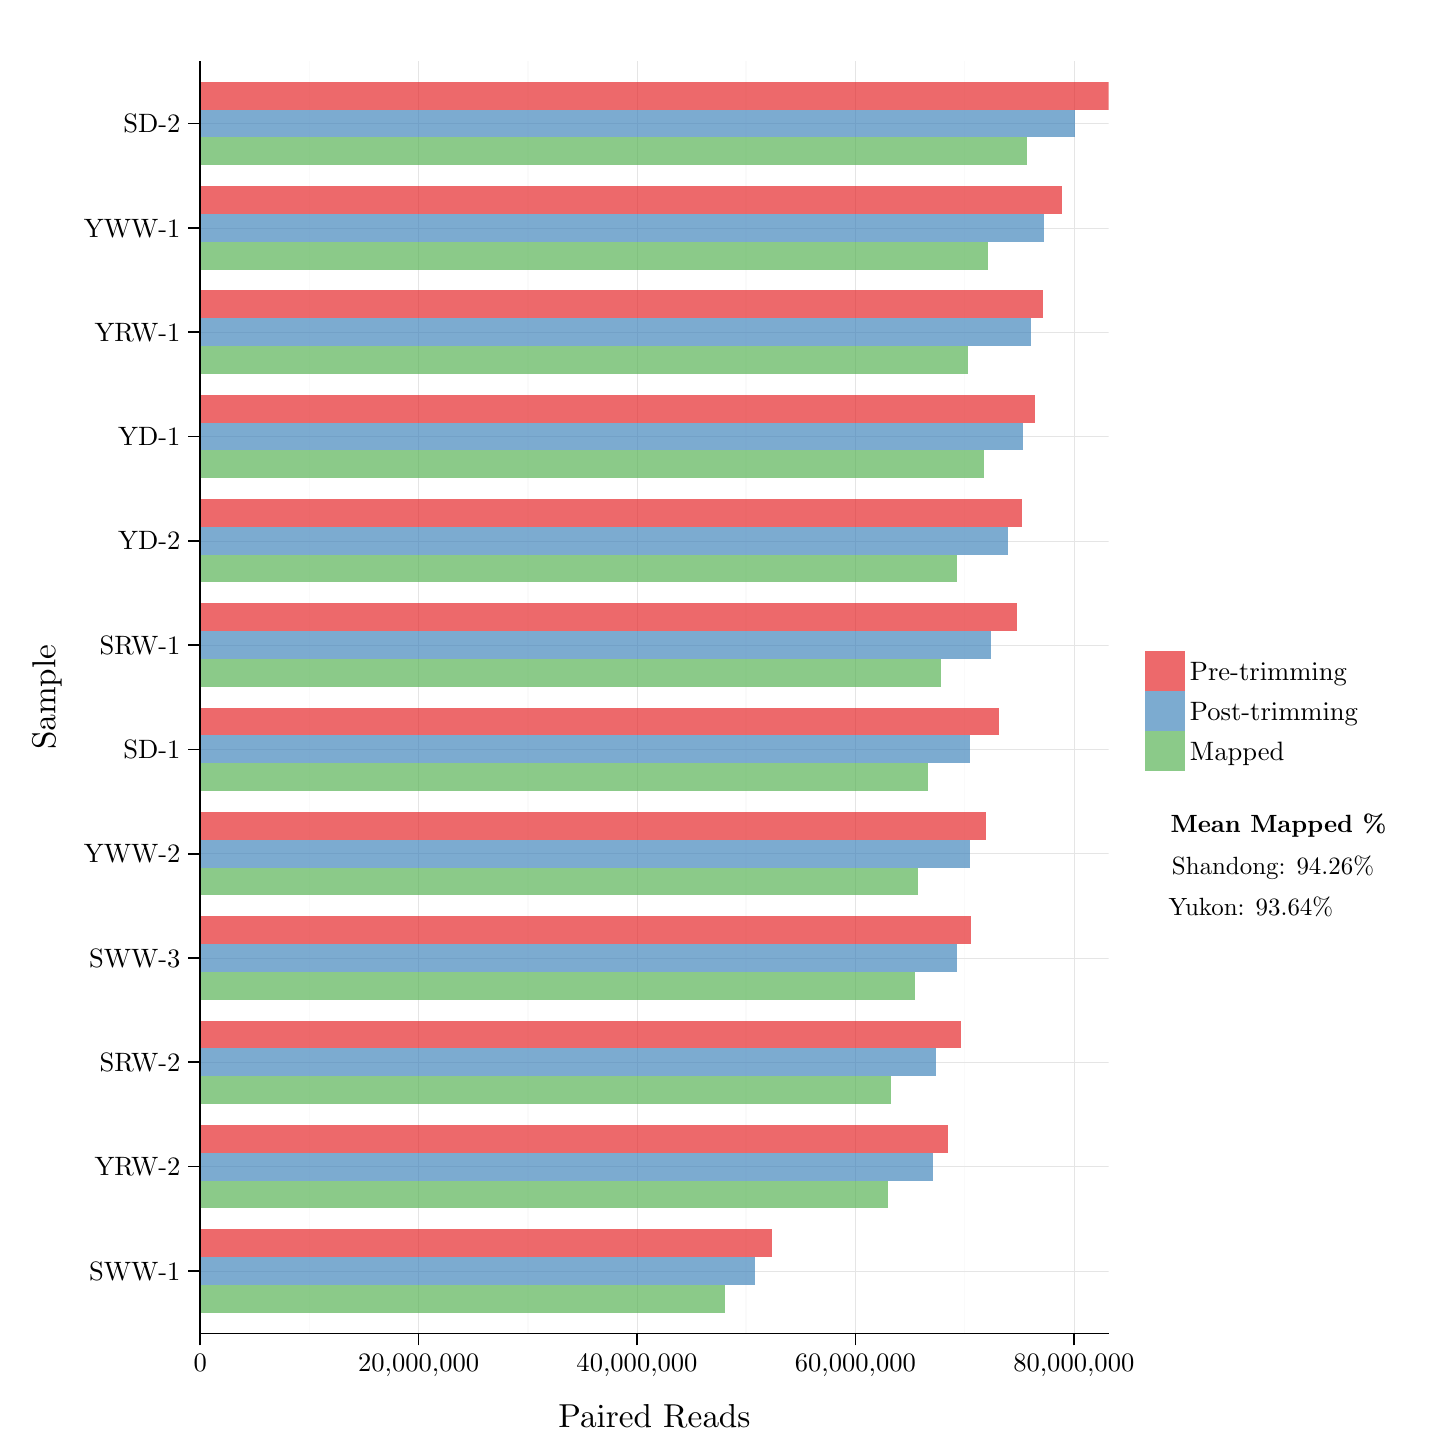
\begin{tikzpicture}[x=1pt,y=1pt]
\definecolor{fillColor}{RGB}{255,255,255}
\path[use as bounding box,fill=fillColor,fill opacity=0.00] (0,0) rectangle (505.89,505.89);
\begin{scope}
\path[clip] (  0.00,  0.00) rectangle (505.89,505.89);
\definecolor{drawColor}{RGB}{255,255,255}
\definecolor{fillColor}{RGB}{255,255,255}

\path[draw=drawColor,line width= 0.6pt,line join=round,line cap=round,fill=fillColor] (  0.00,  0.00) rectangle (505.89,505.89);
\end{scope}
\begin{scope}
\path[clip] ( 62.35, 34.03) rectangle (390.58,493.85);
\definecolor{fillColor}{RGB}{255,255,255}

\path[fill=fillColor] ( 62.35, 34.03) rectangle (390.58,493.85);
\definecolor{drawColor}{gray}{0.98}

\path[draw=drawColor,line width= 0.6pt,line join=round] (101.81, 34.03) --
	(101.81,493.85);

\path[draw=drawColor,line width= 0.6pt,line join=round] (180.72, 34.03) --
	(180.72,493.85);

\path[draw=drawColor,line width= 0.6pt,line join=round] (259.64, 34.03) --
	(259.64,493.85);

\path[draw=drawColor,line width= 0.6pt,line join=round] (338.56, 34.03) --
	(338.56,493.85);
\definecolor{drawColor}{gray}{0.90}

\path[draw=drawColor,line width= 0.2pt,line join=round] ( 62.35, 56.65) --
	(390.58, 56.65);

\path[draw=drawColor,line width= 0.2pt,line join=round] ( 62.35, 94.34) --
	(390.58, 94.34);

\path[draw=drawColor,line width= 0.2pt,line join=round] ( 62.35,132.03) --
	(390.58,132.03);

\path[draw=drawColor,line width= 0.2pt,line join=round] ( 62.35,169.72) --
	(390.58,169.72);

\path[draw=drawColor,line width= 0.2pt,line join=round] ( 62.35,207.41) --
	(390.58,207.41);

\path[draw=drawColor,line width= 0.2pt,line join=round] ( 62.35,245.10) --
	(390.58,245.10);

\path[draw=drawColor,line width= 0.2pt,line join=round] ( 62.35,282.78) --
	(390.58,282.78);

\path[draw=drawColor,line width= 0.2pt,line join=round] ( 62.35,320.47) --
	(390.58,320.47);

\path[draw=drawColor,line width= 0.2pt,line join=round] ( 62.35,358.16) --
	(390.58,358.16);

\path[draw=drawColor,line width= 0.2pt,line join=round] ( 62.35,395.85) --
	(390.58,395.85);

\path[draw=drawColor,line width= 0.2pt,line join=round] ( 62.35,433.54) --
	(390.58,433.54);

\path[draw=drawColor,line width= 0.2pt,line join=round] ( 62.35,471.23) --
	(390.58,471.23);

\path[draw=drawColor,line width= 0.2pt,line join=round] ( 62.35, 34.03) --
	( 62.35,493.85);

\path[draw=drawColor,line width= 0.2pt,line join=round] (141.27, 34.03) --
	(141.27,493.85);

\path[draw=drawColor,line width= 0.2pt,line join=round] (220.18, 34.03) --
	(220.18,493.85);

\path[draw=drawColor,line width= 0.2pt,line join=round] (299.10, 34.03) --
	(299.10,493.85);

\path[draw=drawColor,line width= 0.2pt,line join=round] (378.02, 34.03) --
	(378.02,493.85);
\definecolor{fillColor}{RGB}{228,26,28}

\path[fill=fillColor,fill opacity=0.65] ( 62.35, 61.67) rectangle (268.88, 71.72);
\definecolor{fillColor}{RGB}{55,126,184}

\path[fill=fillColor,fill opacity=0.65] ( 62.35, 51.62) rectangle (262.80, 61.67);
\definecolor{fillColor}{RGB}{77,175,74}

\path[fill=fillColor,fill opacity=0.65] ( 62.35, 41.57) rectangle (252.06, 51.62);
\definecolor{fillColor}{RGB}{228,26,28}

\path[fill=fillColor,fill opacity=0.65] ( 62.35, 99.36) rectangle (332.71,109.41);
\definecolor{fillColor}{RGB}{55,126,184}

\path[fill=fillColor,fill opacity=0.65] ( 62.35, 89.31) rectangle (327.05, 99.36);
\definecolor{fillColor}{RGB}{77,175,74}

\path[fill=fillColor,fill opacity=0.65] ( 62.35, 79.26) rectangle (310.76, 89.31);
\definecolor{fillColor}{RGB}{228,26,28}

\path[fill=fillColor,fill opacity=0.65] ( 62.35,137.05) rectangle (337.38,147.10);
\definecolor{fillColor}{RGB}{55,126,184}

\path[fill=fillColor,fill opacity=0.65] ( 62.35,127.00) rectangle (328.21,137.05);
\definecolor{fillColor}{RGB}{77,175,74}

\path[fill=fillColor,fill opacity=0.65] ( 62.35,116.95) rectangle (311.81,127.00);
\definecolor{fillColor}{RGB}{228,26,28}

\path[fill=fillColor,fill opacity=0.65] ( 62.35,174.74) rectangle (340.76,184.79);
\definecolor{fillColor}{RGB}{55,126,184}

\path[fill=fillColor,fill opacity=0.65] ( 62.35,164.69) rectangle (335.72,174.74);
\definecolor{fillColor}{RGB}{77,175,74}

\path[fill=fillColor,fill opacity=0.65] ( 62.35,154.64) rectangle (320.48,164.69);
\definecolor{fillColor}{RGB}{228,26,28}

\path[fill=fillColor,fill opacity=0.65] ( 62.35,212.43) rectangle (346.32,222.48);
\definecolor{fillColor}{RGB}{55,126,184}

\path[fill=fillColor,fill opacity=0.65] ( 62.35,202.38) rectangle (340.66,212.43);
\definecolor{fillColor}{RGB}{77,175,74}

\path[fill=fillColor,fill opacity=0.65] ( 62.35,192.33) rectangle (321.89,202.38);
\definecolor{fillColor}{RGB}{228,26,28}

\path[fill=fillColor,fill opacity=0.65] ( 62.35,250.12) rectangle (350.94,260.17);
\definecolor{fillColor}{RGB}{55,126,184}

\path[fill=fillColor,fill opacity=0.65] ( 62.35,240.07) rectangle (340.59,250.12);
\definecolor{fillColor}{RGB}{77,175,74}

\path[fill=fillColor,fill opacity=0.65] ( 62.35,230.02) rectangle (325.39,240.07);
\definecolor{fillColor}{RGB}{228,26,28}

\path[fill=fillColor,fill opacity=0.65] ( 62.35,287.81) rectangle (357.31,297.86);
\definecolor{fillColor}{RGB}{55,126,184}

\path[fill=fillColor,fill opacity=0.65] ( 62.35,277.76) rectangle (348.10,287.81);
\definecolor{fillColor}{RGB}{77,175,74}

\path[fill=fillColor,fill opacity=0.65] ( 62.35,267.71) rectangle (330.11,277.76);
\definecolor{fillColor}{RGB}{228,26,28}

\path[fill=fillColor,fill opacity=0.65] ( 62.35,325.50) rectangle (359.19,335.55);
\definecolor{fillColor}{RGB}{55,126,184}

\path[fill=fillColor,fill opacity=0.65] ( 62.35,315.45) rectangle (354.18,325.50);
\definecolor{fillColor}{RGB}{77,175,74}

\path[fill=fillColor,fill opacity=0.65] ( 62.35,305.40) rectangle (335.97,315.45);
\definecolor{fillColor}{RGB}{228,26,28}

\path[fill=fillColor,fill opacity=0.65] ( 62.35,363.19) rectangle (363.83,373.24);
\definecolor{fillColor}{RGB}{55,126,184}

\path[fill=fillColor,fill opacity=0.65] ( 62.35,353.14) rectangle (359.54,363.19);
\definecolor{fillColor}{RGB}{77,175,74}

\path[fill=fillColor,fill opacity=0.65] ( 62.35,343.09) rectangle (345.62,353.14);
\definecolor{fillColor}{RGB}{228,26,28}

\path[fill=fillColor,fill opacity=0.65] ( 62.35,400.88) rectangle (366.85,410.93);
\definecolor{fillColor}{RGB}{55,126,184}

\path[fill=fillColor,fill opacity=0.65] ( 62.35,390.83) rectangle (362.66,400.88);
\definecolor{fillColor}{RGB}{77,175,74}

\path[fill=fillColor,fill opacity=0.65] ( 62.35,380.78) rectangle (339.66,390.83);
\definecolor{fillColor}{RGB}{228,26,28}

\path[fill=fillColor,fill opacity=0.65] ( 62.35,438.57) rectangle (373.57,448.62);
\definecolor{fillColor}{RGB}{55,126,184}

\path[fill=fillColor,fill opacity=0.65] ( 62.35,428.52) rectangle (367.21,438.57);
\definecolor{fillColor}{RGB}{77,175,74}

\path[fill=fillColor,fill opacity=0.65] ( 62.35,418.47) rectangle (346.91,428.52);
\definecolor{fillColor}{RGB}{228,26,28}

\path[fill=fillColor,fill opacity=0.65] ( 62.35,476.26) rectangle (390.58,486.31);
\definecolor{fillColor}{RGB}{55,126,184}

\path[fill=fillColor,fill opacity=0.65] ( 62.35,466.21) rectangle (378.49,476.26);
\definecolor{fillColor}{RGB}{77,175,74}

\path[fill=fillColor,fill opacity=0.65] ( 62.35,456.16) rectangle (360.94,466.21);
\end{scope}
\begin{scope}
\path[clip] (  0.00,  0.00) rectangle (505.89,505.89);
\definecolor{drawColor}{RGB}{0,0,0}

\path[draw=drawColor,line width= 0.6pt,line join=round] ( 62.35, 34.03) --
	( 62.35,493.85);
\end{scope}
\begin{scope}
\path[clip] (  0.00,  0.00) rectangle (505.89,505.89);
\definecolor{drawColor}{RGB}{0,0,0}

\node[text=drawColor,anchor=base east,inner sep=0pt, outer sep=0pt, scale=  0.96] at ( 55.23, 53.34) {SWW-1};

\node[text=drawColor,anchor=base east,inner sep=0pt, outer sep=0pt, scale=  0.96] at ( 55.23, 91.03) {YRW-2};

\node[text=drawColor,anchor=base east,inner sep=0pt, outer sep=0pt, scale=  0.96] at ( 55.23,128.72) {SRW-2};

\node[text=drawColor,anchor=base east,inner sep=0pt, outer sep=0pt, scale=  0.96] at ( 55.23,166.41) {SWW-3};

\node[text=drawColor,anchor=base east,inner sep=0pt, outer sep=0pt, scale=  0.96] at ( 55.23,204.10) {YWW-2};

\node[text=drawColor,anchor=base east,inner sep=0pt, outer sep=0pt, scale=  0.96] at ( 55.23,241.79) {SD-1};

\node[text=drawColor,anchor=base east,inner sep=0pt, outer sep=0pt, scale=  0.96] at ( 55.23,279.48) {SRW-1};

\node[text=drawColor,anchor=base east,inner sep=0pt, outer sep=0pt, scale=  0.96] at ( 55.23,317.17) {YD-2};

\node[text=drawColor,anchor=base east,inner sep=0pt, outer sep=0pt, scale=  0.96] at ( 55.23,354.86) {YD-1};

\node[text=drawColor,anchor=base east,inner sep=0pt, outer sep=0pt, scale=  0.96] at ( 55.23,392.55) {YRW-1};

\node[text=drawColor,anchor=base east,inner sep=0pt, outer sep=0pt, scale=  0.96] at ( 55.23,430.24) {YWW-1};

\node[text=drawColor,anchor=base east,inner sep=0pt, outer sep=0pt, scale=  0.96] at ( 55.23,467.93) {SD-2};
\end{scope}
\begin{scope}
\path[clip] (  0.00,  0.00) rectangle (505.89,505.89);
\definecolor{drawColor}{RGB}{0,0,0}

\path[draw=drawColor,line width= 0.6pt,line join=round] ( 58.08, 56.65) --
	( 62.35, 56.65);

\path[draw=drawColor,line width= 0.6pt,line join=round] ( 58.08, 94.34) --
	( 62.35, 94.34);

\path[draw=drawColor,line width= 0.6pt,line join=round] ( 58.08,132.03) --
	( 62.35,132.03);

\path[draw=drawColor,line width= 0.6pt,line join=round] ( 58.08,169.72) --
	( 62.35,169.72);

\path[draw=drawColor,line width= 0.6pt,line join=round] ( 58.08,207.41) --
	( 62.35,207.41);

\path[draw=drawColor,line width= 0.6pt,line join=round] ( 58.08,245.10) --
	( 62.35,245.10);

\path[draw=drawColor,line width= 0.6pt,line join=round] ( 58.08,282.78) --
	( 62.35,282.78);

\path[draw=drawColor,line width= 0.6pt,line join=round] ( 58.08,320.47) --
	( 62.35,320.47);

\path[draw=drawColor,line width= 0.6pt,line join=round] ( 58.08,358.16) --
	( 62.35,358.16);

\path[draw=drawColor,line width= 0.6pt,line join=round] ( 58.08,395.85) --
	( 62.35,395.85);

\path[draw=drawColor,line width= 0.6pt,line join=round] ( 58.08,433.54) --
	( 62.35,433.54);

\path[draw=drawColor,line width= 0.6pt,line join=round] ( 58.08,471.23) --
	( 62.35,471.23);
\end{scope}
\begin{scope}
\path[clip] (  0.00,  0.00) rectangle (505.89,505.89);
\definecolor{drawColor}{RGB}{0,0,0}

\path[draw=drawColor,line width= 0.6pt,line join=round] ( 62.35, 34.03) --
	(390.58, 34.03);
\end{scope}
\begin{scope}
\path[clip] (  0.00,  0.00) rectangle (505.89,505.89);
\definecolor{drawColor}{RGB}{0,0,0}

\path[draw=drawColor,line width= 0.6pt,line join=round] ( 62.35, 29.77) --
	( 62.35, 34.03);

\path[draw=drawColor,line width= 0.6pt,line join=round] (141.27, 29.77) --
	(141.27, 34.03);

\path[draw=drawColor,line width= 0.6pt,line join=round] (220.18, 29.77) --
	(220.18, 34.03);

\path[draw=drawColor,line width= 0.6pt,line join=round] (299.10, 29.77) --
	(299.10, 34.03);

\path[draw=drawColor,line width= 0.6pt,line join=round] (378.02, 29.77) --
	(378.02, 34.03);
\end{scope}
\begin{scope}
\path[clip] (  0.00,  0.00) rectangle (505.89,505.89);
\definecolor{drawColor}{RGB}{0,0,0}

\node[text=drawColor,anchor=base,inner sep=0pt, outer sep=0pt, scale=  0.96] at ( 62.35, 20.31) {0};

\node[text=drawColor,anchor=base,inner sep=0pt, outer sep=0pt, scale=  0.96] at (141.27, 20.31) {20,000,000};

\node[text=drawColor,anchor=base,inner sep=0pt, outer sep=0pt, scale=  0.96] at (220.18, 20.31) {40,000,000};

\node[text=drawColor,anchor=base,inner sep=0pt, outer sep=0pt, scale=  0.96] at (299.10, 20.31) {60,000,000};

\node[text=drawColor,anchor=base,inner sep=0pt, outer sep=0pt, scale=  0.96] at (378.02, 20.31) {80,000,000};
\end{scope}
\begin{scope}
\path[clip] (  0.00,  0.00) rectangle (505.89,505.89);
\definecolor{drawColor}{RGB}{0,0,0}

\node[text=drawColor,anchor=base,inner sep=0pt, outer sep=0pt, scale=  1.20] at (226.46,  0) {Paired Reads};
\end{scope}
\begin{scope}
\path[clip] (  0.00,  0.00) rectangle (505.89,505.89);
\definecolor{drawColor}{RGB}{0,0,0}

\node[text=drawColor,rotate= 90.00,anchor=base,inner sep=0pt, outer sep=0pt, scale=  1.20] at ( 10,263.94) {Sample};
\end{scope}
\begin{scope}
\path[clip] (  0.00,  0.00) rectangle (505.89,505.89);
\definecolor{drawColor}{RGB}{0,0,0}

\node[text=drawColor,font=\bf,rotate= 0,anchor=base,inner sep=0pt, outer sep=0pt, scale=  0.90] at ( 452,215) {Mean Mapped \%};
\end{scope}
\begin{scope}
\path[clip] (  0.00,  0.00) rectangle (505.89,505.89);
\definecolor{drawColor}{RGB}{0,0,0}

\node[text=drawColor,rotate= 0,anchor=base,inner sep=0pt, outer sep=0pt, scale=  0.90] at ( 450,200) {Shandong: 94.26\%};
\end{scope}
\begin{scope}
\path[clip] (  0.00,  0.00) rectangle (505.89,505.89);
\definecolor{drawColor}{RGB}{0,0,0}

\node[text=drawColor,rotate= 0,anchor=base,inner sep=0pt, outer sep=0pt, scale=  0.90] at ( 442,185) {Yukon: 93.64\%};
\end{scope}
\begin{scope}
\path[clip] (  0.00,  0.00) rectangle (505.89,505.89);
\definecolor{fillColor}{RGB}{255,255,255}

\path[fill=fillColor] (399.45,232.87) rectangle (484.98,295.01);
\end{scope}
\begin{scope}
\path[clip] (  0.00,  0.00) rectangle (505.89,505.89);
\definecolor{drawColor}{gray}{0.80}
\definecolor{fillColor}{RGB}{255,255,255}

%\path[draw=drawColor,line width= 0.6pt,line join=round,line cap=round,fill=fillColor] (403.72,266.05) rectangle (418.17,280.50);
\end{scope}
\begin{scope}
\path[clip] (  0.00,  0.00) rectangle (505.89,505.89);
\definecolor{fillColor}{RGB}{77,175,74}
%green
\path[fill=fillColor,fill opacity=0.65] (403.72,237.14) rectangle (418.17,251.59);

\path[] (403.72,266.05) --
	(418.17,280.50);
\end{scope}
\begin{scope}
\path[clip] (  0.00,  0.00) rectangle (505.89,505.89);
\definecolor{drawColor}{gray}{0.80}
\definecolor{fillColor}{RGB}{255,255,255}

%\path[draw=drawColor,line width= 0.6pt,line join=round,line cap=round,fill=fillColor] (403.72,251.59) rectangle (418.17,266.05);
\end{scope}
\begin{scope}
\path[clip] (  0.00,  0.00) rectangle (505.89,505.89);
\definecolor{fillColor}{RGB}{55,126,184}

%blue
\path[fill=fillColor,fill opacity=0.65] (403.72,251.59) rectangle (418.17,266.05);

\path[] (403.72,251.59) --
	(418.17,266.05);
\end{scope}
\begin{scope}
\path[clip] (  0.00,  0.00) rectangle (505.89,505.89);
\definecolor{drawColor}{gray}{0.80}
\definecolor{fillColor}{RGB}{255,255,255}

%\path[draw=drawColor,line width= 0.6pt,line join=round,line cap=round,fill=fillColor] (403.72,266.05) rectangle (418.17,280.5);
\end{scope}
\begin{scope}
\path[clip] (  0.00,  0.00) rectangle (505.89,505.89);
\definecolor{fillColor}{RGB}{228,26,28}

%red
\path[fill=fillColor,fill opacity=0.65] (403.72,266.05) rectangle (418.17,280.50);

\path[] (403.72,237.14) --
	(418.17,251.59);
\end{scope}
\begin{scope}
\path[clip] (  0.00,  0.00) rectangle (505.89,505.89);
\definecolor{drawColor}{RGB}{0,0,0}

\node[text=drawColor,anchor=base west,inner sep=0pt, outer sep=0pt, scale=  0.96] at (419.98,269.97) {Pre-trimming};
\end{scope}
\begin{scope}
\path[clip] (  0.00,  0.00) rectangle (505.89,505.89);
\definecolor{drawColor}{RGB}{0,0,0}

\node[text=drawColor,anchor=base west,inner sep=0pt, outer sep=0pt, scale=  0.96] at (419.98,255.51) {Post-trimming};
\end{scope}
\begin{scope}
\path[clip] (  0.00,  0.00) rectangle (505.89,505.89);
\definecolor{drawColor}{RGB}{0,0,0}

\node[text=drawColor,anchor=base west,inner sep=0pt, outer sep=0pt, scale=  0.96] at (419.98,241.06) {Mapped};
\end{scope}


\end{tikzpicture}
}
			\caption[Read Processing Statistics]{Read processing and mapping. Values are given as pairs of reads. Samples run on multiple lanes are left separated. The mean percentage of trimmed reads which were sucessfully mapped is indicated for each ecotype.}
			\label{read_stats}
		\end{figure}
	
	Quality trimming of the samples confirmed that the data was relatively high quality (only 2.4\% reads lost due to trimming). Further, mapping was relatively successful, with an average of 94\% of trimmed reads successfully mapping. Since the reference genome was generated using a Shandong ecotype plant, I checked whether there was a difference in the percentage of successfully mapped reads between the Shandong and Yukon samples. It might be expected that Shandong samples would show greater percentage of mapped reads, but there was not enough evidence to say that the two ecotypes mapped with different efficiency (p > 0.1). 
	
	
	\subsection{Batch Effects}
	Since the samples for this study were not all run at the same time, there may be a batch effect which introduces bias within the samples. Unfortunately, the batches are not well mixed (i.e. there is not a good representation of different samples within each batch), which makes it hard to delineate the true differences from the batch differences. However, we can still perform a batch effect analysis and use a conservative approach by removing any genes which show differences due to the batch (script: diff\_gene\_exp.R). When comparing all the samples and batches, we see quite a high number of genes showing differential expression due to batch (~23\% with adjusted p-value < 0.1). However, since batch 4 consists of only Shandong re-watered plants, this might be inflating this value because the batch effect is inherently intertwined with the possible effects of the actual variables we are interested in (ecotype and treatment). I generated a subsetted dataset which removes the SRW samples from the analysis, and re-ran the batch effects just to see how much of a difference these samples would make. When the SRW samples (which are the only samples in batch 4) are removed from the analysis, ~1.3\% genes are showing a difference in expression due to batch. This suggests that the effect is likely magnified because batch 4 contains samples of one type. A way to approach this is to remove the ~1.3\% genes showing differential expression from further analysis, and then to be wary of interesting genes which are part of the 23\% of genes found earlier.
	
	Before removal of the trouble genes, we can perform some cluster analysis to get an idea of our samples and crudely visualize whether there is batch effect. Figure~\ref{pca_batch} provides a principal components analysis (PCA) of the samples, labelled by batch. Although the samples are not distinctly clustering due to batch, there is not even mixing between all of the batches either. However, this would be expected due to the lack of mixing between the samples. For instance, if all the samples in one batch correspond to one ecotype, it would not be expected that this batch's samples would cluster with a batch containing only samples of the other ecotype. This is more evident in Figure~\ref{pca_data} where the samples are labelled based on ecotype and treatment. We can see a clear separation of the ecotypes on PC1, and this provides a more reasonable explanation for the clustering pattern seen in Figure~\ref{pca_batch}. PC2 is able to slightly separate the samples based on treatment condition, but the low variance explained suggests that the ecotype is the major factor in the differences between the samples. 


\begin{figure}
	\centering
	\begin{subfigure}[b]{1\textwidth}
		\centering
			\scalebox{0.5}{% Created by tikzDevice version 0.9 on 2015-12-16 01:29:16
% !TEX encoding = UTF-8 Unicode
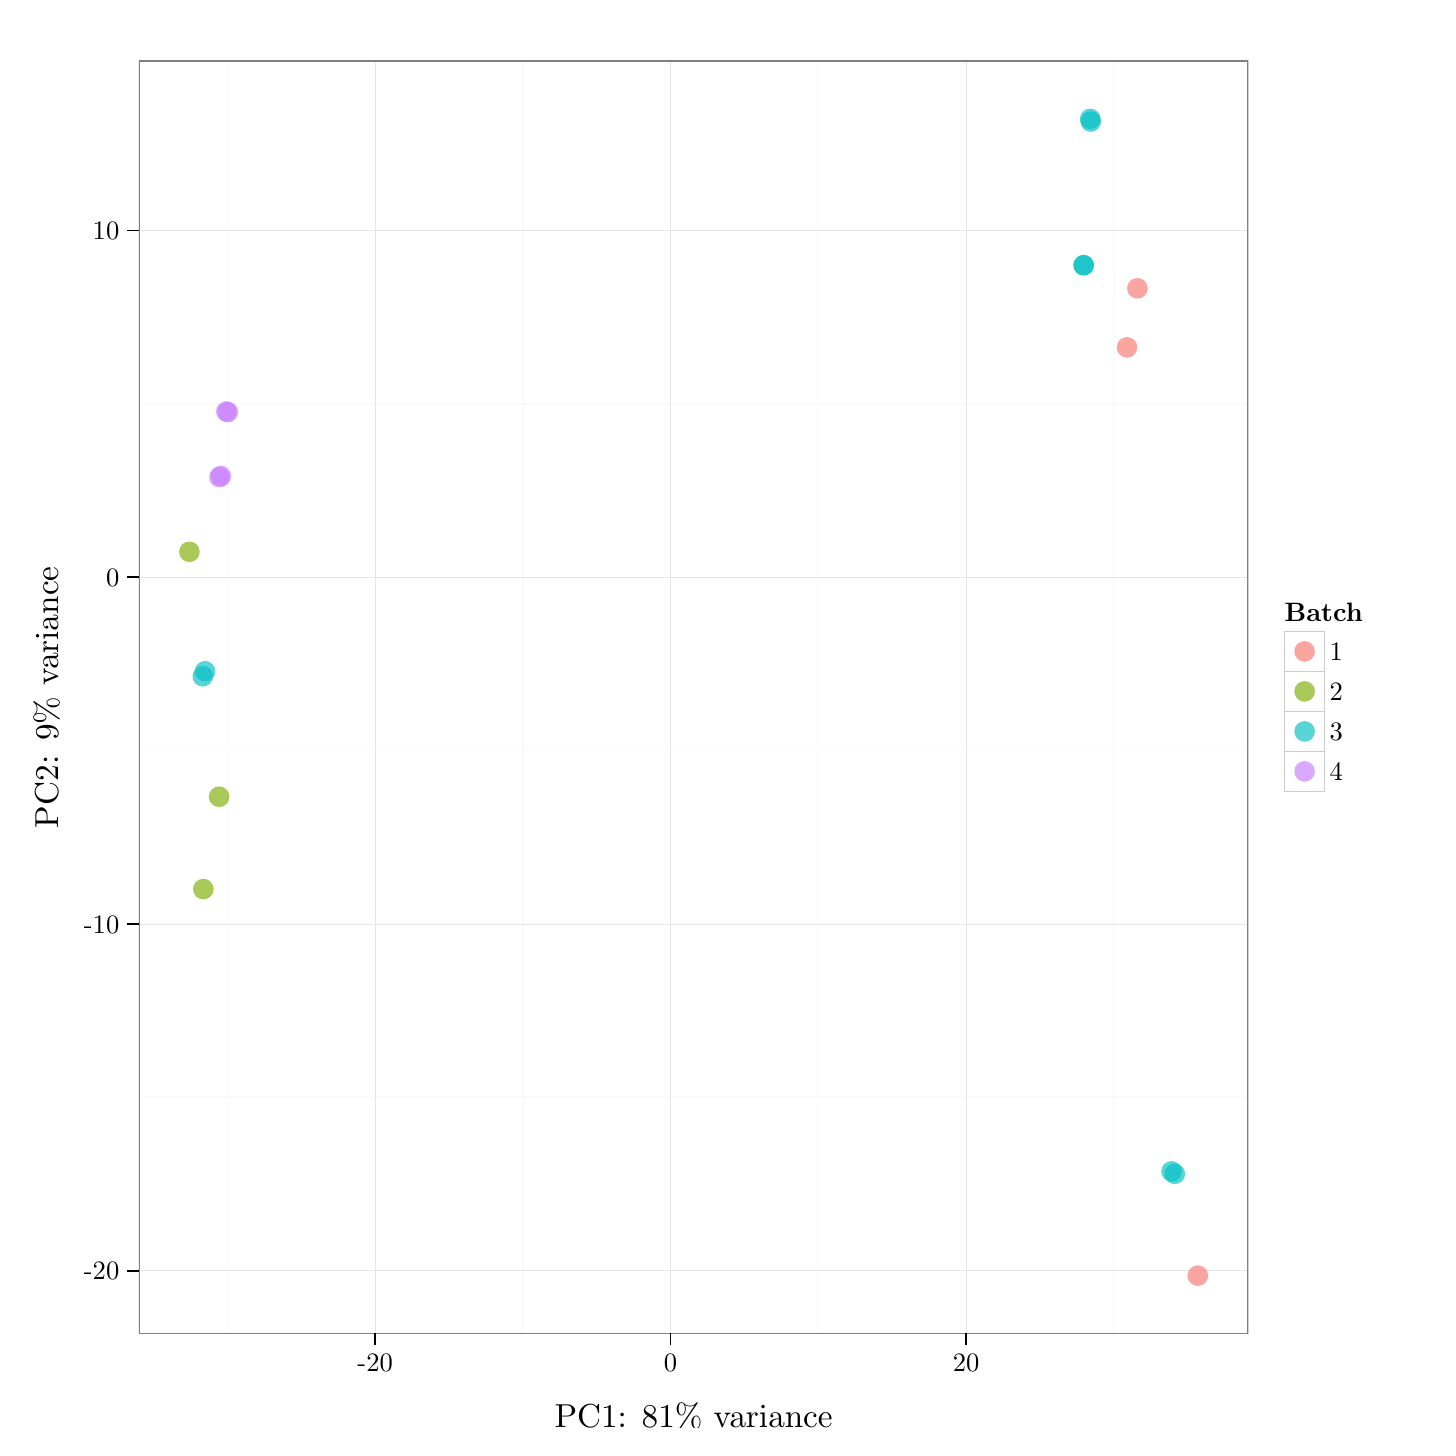
\begin{tikzpicture}[x=1pt,y=1pt]
\definecolor{fillColor}{RGB}{255,255,255}
\path[use as bounding box,fill=fillColor,fill opacity=0.00] (0,0) rectangle (505.89,505.89);
\begin{scope}
\path[clip] (  0.00,  0.00) rectangle (505.89,505.89);
\definecolor{drawColor}{RGB}{255,255,255}
\definecolor{fillColor}{RGB}{255,255,255}

\path[draw=drawColor,line width= 0.6pt,line join=round,line cap=round,fill=fillColor] (  0.00,  0.00) rectangle (505.89,505.89);
\end{scope}
\begin{scope}
\path[clip] ( 40.22, 34.03) rectangle (441.05,493.85);
\definecolor{fillColor}{RGB}{255,255,255}

\path[fill=fillColor] ( 40.22, 34.03) rectangle (441.05,493.85);
\definecolor{drawColor}{gray}{0.98}

\path[draw=drawColor,line width= 0.6pt,line join=round] ( 40.22,119.38) --
	(441.05,119.38);

\path[draw=drawColor,line width= 0.6pt,line join=round] ( 40.22,244.68) --
	(441.05,244.68);

\path[draw=drawColor,line width= 0.6pt,line join=round] ( 40.22,369.97) --
	(441.05,369.97);

\path[draw=drawColor,line width= 0.6pt,line join=round] ( 72.17, 34.03) --
	( 72.17,493.85);

\path[draw=drawColor,line width= 0.6pt,line join=round] (178.94, 34.03) --
	(178.94,493.85);

\path[draw=drawColor,line width= 0.6pt,line join=round] (285.71, 34.03) --
	(285.71,493.85);

\path[draw=drawColor,line width= 0.6pt,line join=round] (392.48, 34.03) --
	(392.48,493.85);
\definecolor{drawColor}{gray}{0.90}

\path[draw=drawColor,line width= 0.2pt,line join=round] ( 40.22, 56.73) --
	(441.05, 56.73);

\path[draw=drawColor,line width= 0.2pt,line join=round] ( 40.22,182.03) --
	(441.05,182.03);

\path[draw=drawColor,line width= 0.2pt,line join=round] ( 40.22,307.32) --
	(441.05,307.32);

\path[draw=drawColor,line width= 0.2pt,line join=round] ( 40.22,432.62) --
	(441.05,432.62);

\path[draw=drawColor,line width= 0.2pt,line join=round] (125.56, 34.03) --
	(125.56,493.85);

\path[draw=drawColor,line width= 0.2pt,line join=round] (232.33, 34.03) --
	(232.33,493.85);

\path[draw=drawColor,line width= 0.2pt,line join=round] (339.10, 34.03) --
	(339.10,493.85);
\definecolor{fillColor}{RGB}{124,174,0}

\path[fill=fillColor,fill opacity=0.65] ( 63.48,194.62) circle (  3.73);

\path[fill=fillColor,fill opacity=0.65] ( 69.19,227.99) circle (  3.73);
\definecolor{fillColor}{RGB}{199,124,255}

\path[fill=fillColor,fill opacity=0.65] ( 72.37,366.95) circle (  3.73);

\path[fill=fillColor,fill opacity=0.65] ( 71.78,367.21) circle (  3.73);

\path[fill=fillColor,fill opacity=0.65] ( 69.28,343.47) circle (  3.73);

\path[fill=fillColor,fill opacity=0.65] ( 69.80,343.90) circle (  3.73);
\definecolor{fillColor}{RGB}{124,174,0}

\path[fill=fillColor,fill opacity=0.65] ( 58.44,316.49) circle (  3.73);
\definecolor{fillColor}{RGB}{0,191,196}

\path[fill=fillColor,fill opacity=0.65] ( 64.10,273.33) circle (  3.73);

\path[fill=fillColor,fill opacity=0.65] ( 63.28,271.50) circle (  3.73);
\definecolor{fillColor}{RGB}{248,118,109}

\path[fill=fillColor,fill opacity=0.65] (422.83, 54.94) circle (  3.73);
\definecolor{fillColor}{RGB}{0,191,196}

\path[fill=fillColor,fill opacity=0.65] (413.32, 92.62) circle (  3.73);

\path[fill=fillColor,fill opacity=0.65] (414.51, 91.73) circle (  3.73);
\definecolor{fillColor}{RGB}{248,118,109}

\path[fill=fillColor,fill opacity=0.65] (397.24,390.37) circle (  3.73);
\definecolor{fillColor}{RGB}{0,191,196}

\path[fill=fillColor,fill opacity=0.65] (384.15,471.97) circle (  3.73);

\path[fill=fillColor,fill opacity=0.65] (383.95,472.94) circle (  3.73);
\definecolor{fillColor}{RGB}{248,118,109}

\path[fill=fillColor,fill opacity=0.65] (400.99,411.70) circle (  3.73);
\definecolor{fillColor}{RGB}{0,191,196}

\path[fill=fillColor,fill opacity=0.65] (381.56,420.04) circle (  3.73);

\path[fill=fillColor,fill opacity=0.65] (381.59,420.04) circle (  3.73);
\definecolor{drawColor}{gray}{0.50}

\path[draw=drawColor,line width= 0.6pt,line join=round,line cap=round] ( 40.22, 34.03) rectangle (441.05,493.85);
\end{scope}
\begin{scope}
\path[clip] (  0.00,  0.00) rectangle (505.89,505.89);
\definecolor{drawColor}{RGB}{0,0,0}

\node[text=drawColor,anchor=base east,inner sep=0pt, outer sep=0pt, scale=  0.96] at ( 33.11, 53.42) {-20};

\node[text=drawColor,anchor=base east,inner sep=0pt, outer sep=0pt, scale=  0.96] at ( 33.11,178.72) {-10};

\node[text=drawColor,anchor=base east,inner sep=0pt, outer sep=0pt, scale=  0.96] at ( 33.11,304.02) {0};

\node[text=drawColor,anchor=base east,inner sep=0pt, outer sep=0pt, scale=  0.96] at ( 33.11,429.32) {10};
\end{scope}
\begin{scope}
\path[clip] (  0.00,  0.00) rectangle (505.89,505.89);
\definecolor{drawColor}{RGB}{0,0,0}

\path[draw=drawColor,line width= 0.6pt,line join=round] ( 35.95, 56.73) --
	( 40.22, 56.73);

\path[draw=drawColor,line width= 0.6pt,line join=round] ( 35.95,182.03) --
	( 40.22,182.03);

\path[draw=drawColor,line width= 0.6pt,line join=round] ( 35.95,307.32) --
	( 40.22,307.32);

\path[draw=drawColor,line width= 0.6pt,line join=round] ( 35.95,432.62) --
	( 40.22,432.62);
\end{scope}
\begin{scope}
\path[clip] (  0.00,  0.00) rectangle (505.89,505.89);
\definecolor{drawColor}{RGB}{0,0,0}

\path[draw=drawColor,line width= 0.6pt,line join=round] (125.56, 29.77) --
	(125.56, 34.03);

\path[draw=drawColor,line width= 0.6pt,line join=round] (232.33, 29.77) --
	(232.33, 34.03);

\path[draw=drawColor,line width= 0.6pt,line join=round] (339.10, 29.77) --
	(339.10, 34.03);
\end{scope}
\begin{scope}
\path[clip] (  0.00,  0.00) rectangle (505.89,505.89);
\definecolor{drawColor}{RGB}{0,0,0}

\node[text=drawColor,anchor=base,inner sep=0pt, outer sep=0pt, scale=  0.96] at (125.56, 20.31) {-20};

\node[text=drawColor,anchor=base,inner sep=0pt, outer sep=0pt, scale=  0.96] at (232.33, 20.31) {0};

\node[text=drawColor,anchor=base,inner sep=0pt, outer sep=0pt, scale=  0.96] at (339.10, 20.31) {20};
\end{scope}
\begin{scope}
\path[clip] (  0.00,  0.00) rectangle (505.89,505.89);
\definecolor{drawColor}{RGB}{0,0,0}

\node[text=drawColor,anchor=base,inner sep=0pt, outer sep=0pt, scale=  1.20] at (240.64,  0) {PC1: 81\% variance};
\end{scope}
\begin{scope}
\path[clip] (  0.00,  0.00) rectangle (505.89,505.89);
\definecolor{drawColor}{RGB}{0,0,0}

\node[text=drawColor,rotate= 90.00,anchor=base,inner sep=0pt, outer sep=0pt, scale=  1.20] at ( 11,263.94) {PC2: 9\% variance};
\end{scope}
\begin{scope}
\path[clip] (  0.00,  0.00) rectangle (505.89,505.89);
\definecolor{fillColor}{RGB}{255,255,255}

\path[fill=fillColor] (449.92,225.64) rectangle (484.98,302.23);
\end{scope}
\begin{scope}
\path[clip] (  0.00,  0.00) rectangle (505.89,505.89);
\definecolor{drawColor}{RGB}{0,0,0}

\node[text=drawColor,anchor=base west,inner sep=0pt, outer sep=0pt, scale=  0.96] at (454.19,291.34) {\bfseries Batch};
\end{scope}
\begin{scope}
\path[clip] (  0.00,  0.00) rectangle (505.89,505.89);
\definecolor{drawColor}{gray}{0.80}
\definecolor{fillColor}{RGB}{255,255,255}

\path[draw=drawColor,line width= 0.6pt,line join=round,line cap=round,fill=fillColor] (454.19,273.27) rectangle (468.64,287.73);
\end{scope}
\begin{scope}
\path[clip] (  0.00,  0.00) rectangle (505.89,505.89);
\definecolor{fillColor}{RGB}{248,118,109}

\path[fill=fillColor,fill opacity=0.65] (461.42,280.50) circle (  3.73);
\end{scope}
\begin{scope}
\path[clip] (  0.00,  0.00) rectangle (505.89,505.89);
\definecolor{drawColor}{gray}{0.80}
\definecolor{fillColor}{RGB}{255,255,255}

\path[draw=drawColor,line width= 0.6pt,line join=round,line cap=round,fill=fillColor] (454.19,258.82) rectangle (468.64,273.27);
\end{scope}
\begin{scope}
\path[clip] (  0.00,  0.00) rectangle (505.89,505.89);
\definecolor{fillColor}{RGB}{124,174,0}

\path[fill=fillColor,fill opacity=0.65] (461.42,266.05) circle (  3.73);
\end{scope}
\begin{scope}
\path[clip] (  0.00,  0.00) rectangle (505.89,505.89);
\definecolor{drawColor}{gray}{0.80}
\definecolor{fillColor}{RGB}{255,255,255}

\path[draw=drawColor,line width= 0.6pt,line join=round,line cap=round,fill=fillColor] (454.19,244.37) rectangle (468.64,258.82);
\end{scope}
\begin{scope}
\path[clip] (  0.00,  0.00) rectangle (505.89,505.89);
\definecolor{fillColor}{RGB}{0,191,196}

\path[fill=fillColor,fill opacity=0.65] (461.42,251.59) circle (  3.73);
\end{scope}
\begin{scope}
\path[clip] (  0.00,  0.00) rectangle (505.89,505.89);
\definecolor{drawColor}{gray}{0.80}
\definecolor{fillColor}{RGB}{255,255,255}

\path[draw=drawColor,line width= 0.6pt,line join=round,line cap=round,fill=fillColor] (454.19,229.91) rectangle (468.64,244.37);
\end{scope}
\begin{scope}
\path[clip] (  0.00,  0.00) rectangle (505.89,505.89);
\definecolor{fillColor}{RGB}{199,124,255}

\path[fill=fillColor,fill opacity=0.65] (461.42,237.14) circle (  3.73);
\end{scope}
\begin{scope}
\path[clip] (  0.00,  0.00) rectangle (505.89,505.89);
\definecolor{drawColor}{RGB}{0,0,0}

\node[text=drawColor,anchor=base west,inner sep=0pt, outer sep=0pt, scale=  0.96] at (470.45,277.20) {1};
\end{scope}
\begin{scope}
\path[clip] (  0.00,  0.00) rectangle (505.89,505.89);
\definecolor{drawColor}{RGB}{0,0,0}

\node[text=drawColor,anchor=base west,inner sep=0pt, outer sep=0pt, scale=  0.96] at (470.45,262.74) {2};
\end{scope}
\begin{scope}
\path[clip] (  0.00,  0.00) rectangle (505.89,505.89);
\definecolor{drawColor}{RGB}{0,0,0}

\node[text=drawColor,anchor=base west,inner sep=0pt, outer sep=0pt, scale=  0.96] at (470.45,248.29) {3};
\end{scope}
\begin{scope}
\path[clip] (  0.00,  0.00) rectangle (505.89,505.89);
\definecolor{drawColor}{RGB}{0,0,0}

\node[text=drawColor,anchor=base west,inner sep=0pt, outer sep=0pt, scale=  0.96] at (470.45,233.83) {4};
\end{scope}
\end{tikzpicture}
}
		\caption{}
		\label{pca_batch}
	\end{subfigure}
	~ %add desired spacing between images, e. g. ~, \quad, \qquad, \hfill etc. 
	%(or a blank line to force the subfigure onto a new line)
	\begin{subfigure}[b]{1\textwidth}
		\centering
			\scalebox{0.5}{% Created by tikzDevice version 0.9 on 2015-12-16 01:29:24
% !TEX encoding = UTF-8 Unicode
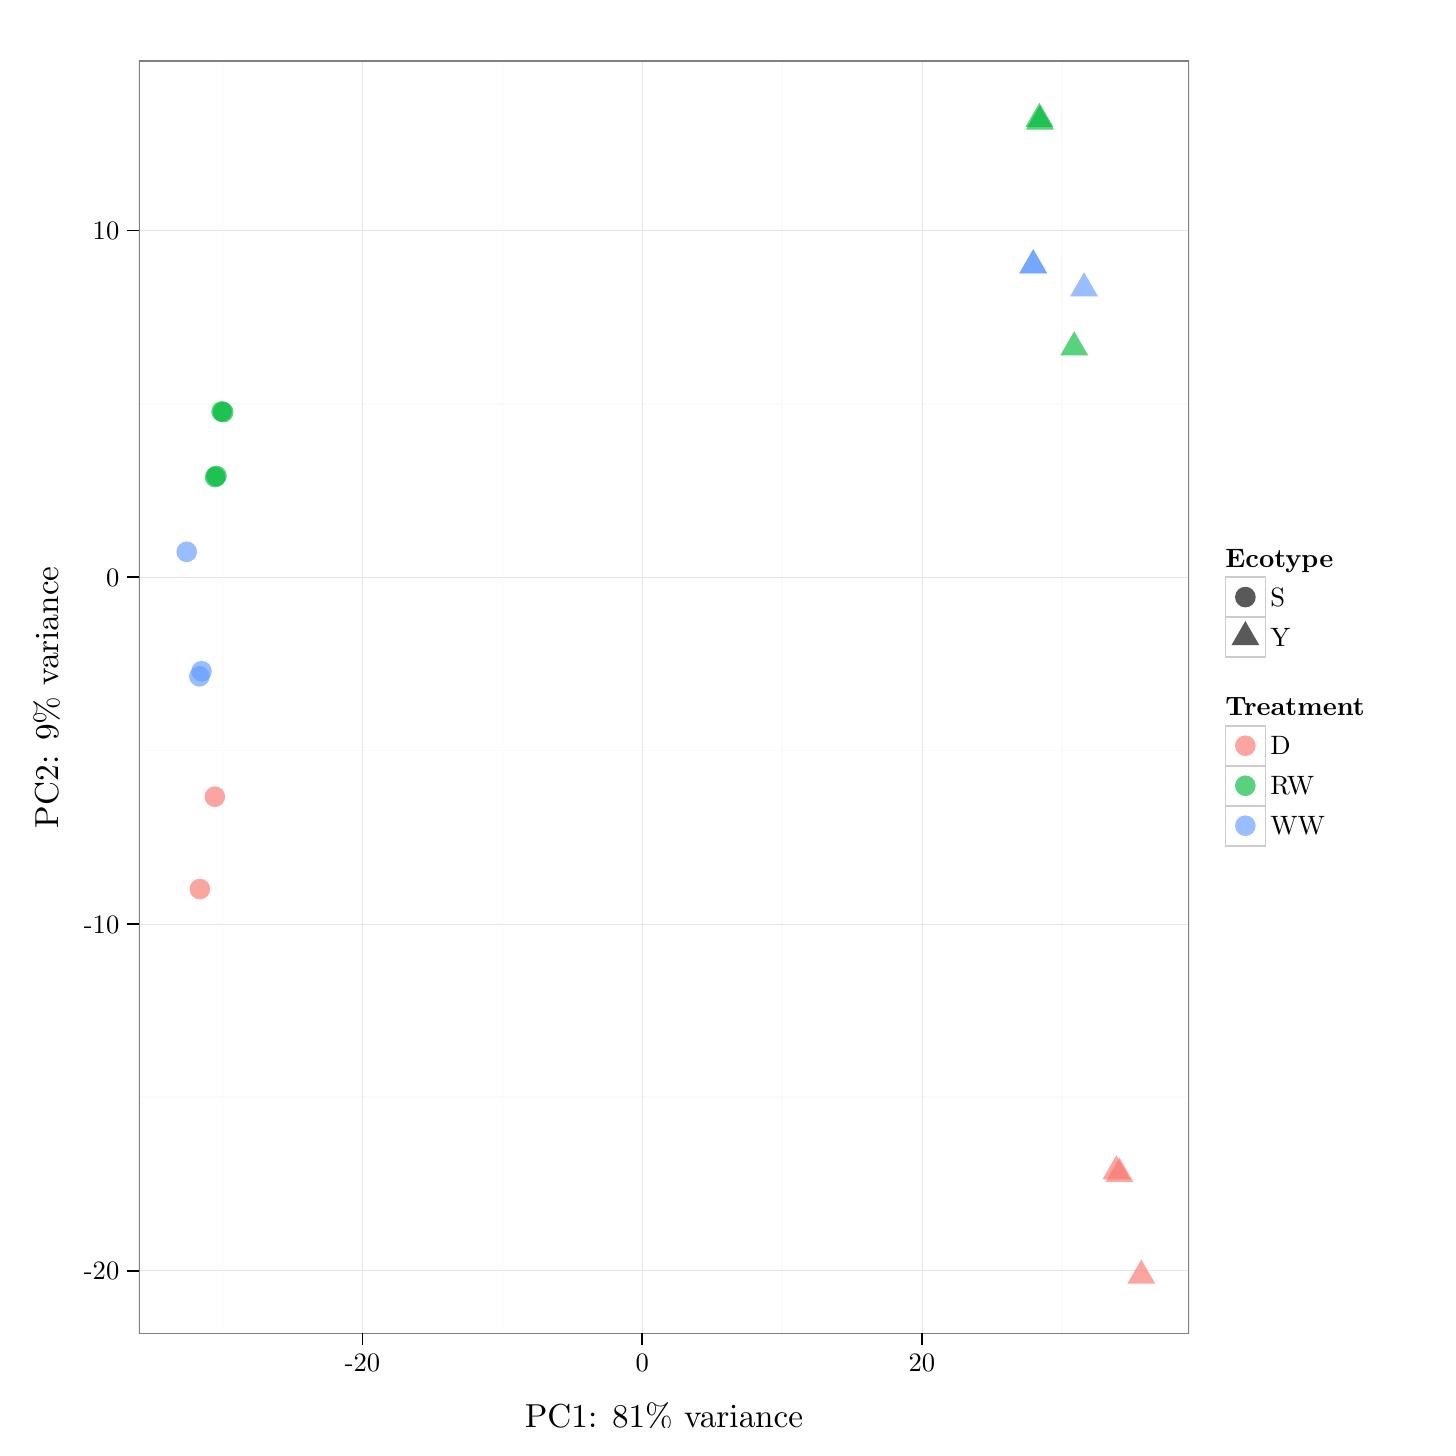
\begin{tikzpicture}[x=1pt,y=1pt]
\definecolor{fillColor}{RGB}{255,255,255}
\path[use as bounding box,fill=fillColor,fill opacity=0.00] (0,0) rectangle (505.89,505.89);
\begin{scope}
\path[clip] (  0.00,  0.00) rectangle (505.89,505.89);
\definecolor{drawColor}{RGB}{255,255,255}
\definecolor{fillColor}{RGB}{255,255,255}

\path[draw=drawColor,line width= 0.6pt,line join=round,line cap=round,fill=fillColor] (  0.00,  0.00) rectangle (505.89,505.89);
\end{scope}
\begin{scope}
\path[clip] ( 40.22, 34.03) rectangle (419.65,493.85);
\definecolor{fillColor}{RGB}{255,255,255}

\path[fill=fillColor] ( 40.22, 34.03) rectangle (419.65,493.85);
\definecolor{drawColor}{gray}{0.98}

\path[draw=drawColor,line width= 0.6pt,line join=round] ( 40.22,119.38) --
	(419.65,119.38);

\path[draw=drawColor,line width= 0.6pt,line join=round] ( 40.22,244.68) --
	(419.65,244.68);

\path[draw=drawColor,line width= 0.6pt,line join=round] ( 40.22,369.97) --
	(419.65,369.97);

\path[draw=drawColor,line width= 0.6pt,line join=round] ( 70.46, 34.03) --
	( 70.46,493.85);

\path[draw=drawColor,line width= 0.6pt,line join=round] (171.53, 34.03) --
	(171.53,493.85);

\path[draw=drawColor,line width= 0.6pt,line join=round] (272.60, 34.03) --
	(272.60,493.85);

\path[draw=drawColor,line width= 0.6pt,line join=round] (373.67, 34.03) --
	(373.67,493.85);
\definecolor{drawColor}{gray}{0.90}

\path[draw=drawColor,line width= 0.2pt,line join=round] ( 40.22, 56.73) --
	(419.65, 56.73);

\path[draw=drawColor,line width= 0.2pt,line join=round] ( 40.22,182.03) --
	(419.65,182.03);

\path[draw=drawColor,line width= 0.2pt,line join=round] ( 40.22,307.32) --
	(419.65,307.32);

\path[draw=drawColor,line width= 0.2pt,line join=round] ( 40.22,432.62) --
	(419.65,432.62);

\path[draw=drawColor,line width= 0.2pt,line join=round] (121.00, 34.03) --
	(121.00,493.85);

\path[draw=drawColor,line width= 0.2pt,line join=round] (222.06, 34.03) --
	(222.06,493.85);

\path[draw=drawColor,line width= 0.2pt,line join=round] (323.13, 34.03) --
	(323.13,493.85);
\definecolor{fillColor}{RGB}{248,118,109}

\path[fill=fillColor,fill opacity=0.65] ( 62.23,194.62) circle (  3.73);

\path[fill=fillColor,fill opacity=0.65] ( 67.64,227.99) circle (  3.73);
\definecolor{fillColor}{RGB}{0,186,56}

\path[fill=fillColor,fill opacity=0.65] ( 70.65,366.95) circle (  3.73);

\path[fill=fillColor,fill opacity=0.65] ( 70.09,367.21) circle (  3.73);

\path[fill=fillColor,fill opacity=0.65] ( 67.73,343.47) circle (  3.73);

\path[fill=fillColor,fill opacity=0.65] ( 68.22,343.90) circle (  3.73);
\definecolor{fillColor}{RGB}{97,156,255}

\path[fill=fillColor,fill opacity=0.65] ( 57.47,316.49) circle (  3.73);

\path[fill=fillColor,fill opacity=0.65] ( 62.82,273.33) circle (  3.73);

\path[fill=fillColor,fill opacity=0.65] ( 62.05,271.50) circle (  3.73);
\definecolor{fillColor}{RGB}{248,118,109}

\path[fill=fillColor,fill opacity=0.65] (402.40, 60.74) --
	(407.43, 52.03) --
	(397.37, 52.03) --
	cycle;

\path[fill=fillColor,fill opacity=0.65] (393.39, 98.43) --
	(398.42, 89.72) --
	(388.36, 89.72) --
	cycle;

\path[fill=fillColor,fill opacity=0.65] (394.52, 97.54) --
	(399.55, 88.83) --
	(389.49, 88.83) --
	cycle;
\definecolor{fillColor}{RGB}{0,186,56}

\path[fill=fillColor,fill opacity=0.65] (378.17,396.18) --
	(383.20,387.47) --
	(373.14,387.47) --
	cycle;

\path[fill=fillColor,fill opacity=0.65] (365.78,477.78) --
	(370.81,469.07) --
	(360.75,469.07) --
	cycle;

\path[fill=fillColor,fill opacity=0.65] (365.59,478.75) --
	(370.62,470.04) --
	(360.56,470.04) --
	cycle;
\definecolor{fillColor}{RGB}{97,156,255}

\path[fill=fillColor,fill opacity=0.65] (381.72,417.51) --
	(386.75,408.80) --
	(376.69,408.80) --
	cycle;

\path[fill=fillColor,fill opacity=0.65] (363.33,425.85) --
	(368.36,417.14) --
	(358.30,417.14) --
	cycle;

\path[fill=fillColor,fill opacity=0.65] (363.36,425.85) --
	(368.39,417.14) --
	(358.33,417.14) --
	cycle;
\definecolor{drawColor}{gray}{0.50}

\path[draw=drawColor,line width= 0.6pt,line join=round,line cap=round] ( 40.22, 34.03) rectangle (419.65,493.85);
\end{scope}
\begin{scope}
\path[clip] (  0.00,  0.00) rectangle (505.89,505.89);
\definecolor{drawColor}{RGB}{0,0,0}

\node[text=drawColor,anchor=base east,inner sep=0pt, outer sep=0pt, scale=  0.96] at ( 33.11, 53.42) {-20};

\node[text=drawColor,anchor=base east,inner sep=0pt, outer sep=0pt, scale=  0.96] at ( 33.11,178.72) {-10};

\node[text=drawColor,anchor=base east,inner sep=0pt, outer sep=0pt, scale=  0.96] at ( 33.11,304.02) {0};

\node[text=drawColor,anchor=base east,inner sep=0pt, outer sep=0pt, scale=  0.96] at ( 33.11,429.32) {10};
\end{scope}
\begin{scope}
\path[clip] (  0.00,  0.00) rectangle (505.89,505.89);
\definecolor{drawColor}{RGB}{0,0,0}

\path[draw=drawColor,line width= 0.6pt,line join=round] ( 35.95, 56.73) --
	( 40.22, 56.73);

\path[draw=drawColor,line width= 0.6pt,line join=round] ( 35.95,182.03) --
	( 40.22,182.03);

\path[draw=drawColor,line width= 0.6pt,line join=round] ( 35.95,307.32) --
	( 40.22,307.32);

\path[draw=drawColor,line width= 0.6pt,line join=round] ( 35.95,432.62) --
	( 40.22,432.62);
\end{scope}
\begin{scope}
\path[clip] (  0.00,  0.00) rectangle (505.89,505.89);
\definecolor{drawColor}{RGB}{0,0,0}

\path[draw=drawColor,line width= 0.6pt,line join=round] (121.00, 29.77) --
	(121.00, 34.03);

\path[draw=drawColor,line width= 0.6pt,line join=round] (222.06, 29.77) --
	(222.06, 34.03);

\path[draw=drawColor,line width= 0.6pt,line join=round] (323.13, 29.77) --
	(323.13, 34.03);
\end{scope}
\begin{scope}
\path[clip] (  0.00,  0.00) rectangle (505.89,505.89);
\definecolor{drawColor}{RGB}{0,0,0}

\node[text=drawColor,anchor=base,inner sep=0pt, outer sep=0pt, scale=  0.96] at (121.00, 20.31) {-20};

\node[text=drawColor,anchor=base,inner sep=0pt, outer sep=0pt, scale=  0.96] at (222.06, 20.31) {0};

\node[text=drawColor,anchor=base,inner sep=0pt, outer sep=0pt, scale=  0.96] at (323.13, 20.31) {20};
\end{scope}
\begin{scope}
\path[clip] (  0.00,  0.00) rectangle (505.89,505.89);
\definecolor{drawColor}{RGB}{0,0,0}

\node[text=drawColor,anchor=base,inner sep=0pt, outer sep=0pt, scale=  1.20] at (229.93,  0) {PC1: 81\% variance};
\end{scope}
\begin{scope}
\path[clip] (  0.00,  0.00) rectangle (505.89,505.89);
\definecolor{drawColor}{RGB}{0,0,0}

\node[text=drawColor,rotate= 90.00,anchor=base,inner sep=0pt, outer sep=0pt, scale=  1.20] at ( 11,263.94) {PC2: 9\% variance};
\end{scope}
\begin{scope}
\path[clip] (  0.00,  0.00) rectangle (505.89,505.89);
\definecolor{fillColor}{RGB}{255,255,255}

\path[fill=fillColor] (428.51,274.18) rectangle (473.84,321.86);
\end{scope}
\begin{scope}
\path[clip] (  0.00,  0.00) rectangle (505.89,505.89);
\definecolor{drawColor}{RGB}{0,0,0}

\node[text=drawColor,anchor=base west,inner sep=0pt, outer sep=0pt, scale=  0.96] at (432.78,310.97) {\bfseries Ecotype};
\end{scope}
\begin{scope}
\path[clip] (  0.00,  0.00) rectangle (505.89,505.89);
\definecolor{drawColor}{gray}{0.80}
\definecolor{fillColor}{RGB}{255,255,255}

\path[draw=drawColor,line width= 0.6pt,line join=round,line cap=round,fill=fillColor] (432.78,292.90) rectangle (447.23,307.35);
\end{scope}
\begin{scope}
\path[clip] (  0.00,  0.00) rectangle (505.89,505.89);
\definecolor{fillColor}{RGB}{0,0,0}

\path[fill=fillColor,fill opacity=0.65] (440.01,300.13) circle (  3.73);
\end{scope}
\begin{scope}
\path[clip] (  0.00,  0.00) rectangle (505.89,505.89);
\definecolor{drawColor}{gray}{0.80}
\definecolor{fillColor}{RGB}{255,255,255}

\path[draw=drawColor,line width= 0.6pt,line join=round,line cap=round,fill=fillColor] (432.78,278.45) rectangle (447.23,292.90);
\end{scope}
\begin{scope}
\path[clip] (  0.00,  0.00) rectangle (505.89,505.89);
\definecolor{fillColor}{RGB}{0,0,0}

\path[fill=fillColor,fill opacity=0.65] (440.01,291.48) --
	(445.04,282.77) --
	(434.98,282.77) --
	cycle;
\end{scope}
\begin{scope}
\path[clip] (  0.00,  0.00) rectangle (505.89,505.89);
\definecolor{drawColor}{RGB}{0,0,0}

\node[text=drawColor,anchor=base west,inner sep=0pt, outer sep=0pt, scale=  0.96] at (449.04,296.82) {S};
\end{scope}
\begin{scope}
\path[clip] (  0.00,  0.00) rectangle (505.89,505.89);
\definecolor{drawColor}{RGB}{0,0,0}

\node[text=drawColor,anchor=base west,inner sep=0pt, outer sep=0pt, scale=  0.96] at (449.04,282.37) {Y};
\end{scope}
\begin{scope}
\path[clip] (  0.00,  0.00) rectangle (505.89,505.89);
\definecolor{fillColor}{RGB}{255,255,255}

\path[fill=fillColor] (428.51,206.02) rectangle (484.98,268.16);
\end{scope}
\begin{scope}
\path[clip] (  0.00,  0.00) rectangle (505.89,505.89);
\definecolor{drawColor}{RGB}{0,0,0}

\node[text=drawColor,anchor=base west,inner sep=0pt, outer sep=0pt, scale=  0.96] at (432.78,257.26) {\bfseries Treatment};
\end{scope}
\begin{scope}
\path[clip] (  0.00,  0.00) rectangle (505.89,505.89);
\definecolor{drawColor}{gray}{0.80}
\definecolor{fillColor}{RGB}{255,255,255}

\path[draw=drawColor,line width= 0.6pt,line join=round,line cap=round,fill=fillColor] (432.78,239.20) rectangle (447.23,253.65);
\end{scope}
\begin{scope}
\path[clip] (  0.00,  0.00) rectangle (505.89,505.89);
\definecolor{fillColor}{RGB}{248,118,109}

\path[fill=fillColor,fill opacity=0.65] (440.01,246.42) circle (  3.73);
\end{scope}
\begin{scope}
\path[clip] (  0.00,  0.00) rectangle (505.89,505.89);
\definecolor{drawColor}{gray}{0.80}
\definecolor{fillColor}{RGB}{255,255,255}

\path[draw=drawColor,line width= 0.6pt,line join=round,line cap=round,fill=fillColor] (432.78,224.74) rectangle (447.23,239.20);
\end{scope}
\begin{scope}
\path[clip] (  0.00,  0.00) rectangle (505.89,505.89);
\definecolor{fillColor}{RGB}{0,186,56}

\path[fill=fillColor,fill opacity=0.65] (440.01,231.97) circle (  3.73);
\end{scope}
\begin{scope}
\path[clip] (  0.00,  0.00) rectangle (505.89,505.89);
\definecolor{drawColor}{gray}{0.80}
\definecolor{fillColor}{RGB}{255,255,255}

\path[draw=drawColor,line width= 0.6pt,line join=round,line cap=round,fill=fillColor] (432.78,210.29) rectangle (447.23,224.74);
\end{scope}
\begin{scope}
\path[clip] (  0.00,  0.00) rectangle (505.89,505.89);
\definecolor{fillColor}{RGB}{97,156,255}

\path[fill=fillColor,fill opacity=0.65] (440.01,217.51) circle (  3.73);
\end{scope}
\begin{scope}
\path[clip] (  0.00,  0.00) rectangle (505.89,505.89);
\definecolor{drawColor}{RGB}{0,0,0}

\node[text=drawColor,anchor=base west,inner sep=0pt, outer sep=0pt, scale=  0.96] at (449.04,243.12) {D};
\end{scope}
\begin{scope}
\path[clip] (  0.00,  0.00) rectangle (505.89,505.89);
\definecolor{drawColor}{RGB}{0,0,0}

\node[text=drawColor,anchor=base west,inner sep=0pt, outer sep=0pt, scale=  0.96] at (449.04,228.66) {RW};
\end{scope}
\begin{scope}
\path[clip] (  0.00,  0.00) rectangle (505.89,505.89);
\definecolor{drawColor}{RGB}{0,0,0}

\node[text=drawColor,anchor=base west,inner sep=0pt, outer sep=0pt, scale=  0.96] at (449.04,214.21) {WW};
\end{scope}
\end{tikzpicture}
}
		\caption{}
		\label{pca_data}
	\end{subfigure}
	\caption[Cluster analysis with PCA]{Principal components analysis of samples labelled based on \textbf{a)} batch or \textbf{b)} ecotype and treatment}
	\label{pca}
\end{figure}
		
	The samples can also be visualized using a heatmap (Figure~\ref{heatmap}.)	This further presents the separation of the samples based on ecotype, with the Shandong and Yukon ecotype samples clustering together. As well, the SRW samples show a high degree of similarity to each other and form a distinct cluster from the other samples. Again, we cannot be certain of the degree to which batch effects may be playing a role in the separation of the SRW samples, but the pattern of samples clustering together based on the variables of interest and not batch is a good sign. Interestingly, an SWW samples which was run in batch 2 clustered more closely with an SD sample which was also run on batch 2 rather than on the other SWW samples run on batch 3. This hints at the possibility of a batch effect and supports the removal of the ~1.3\% genes discussed earlier.
		
		\begin{figure}[H]
			\centering
			\scalebox{0.7}{% Created by tikzDevice version 0.9 on 2015-12-15 14:25:43
% !TEX encoding = UTF-8 Unicode
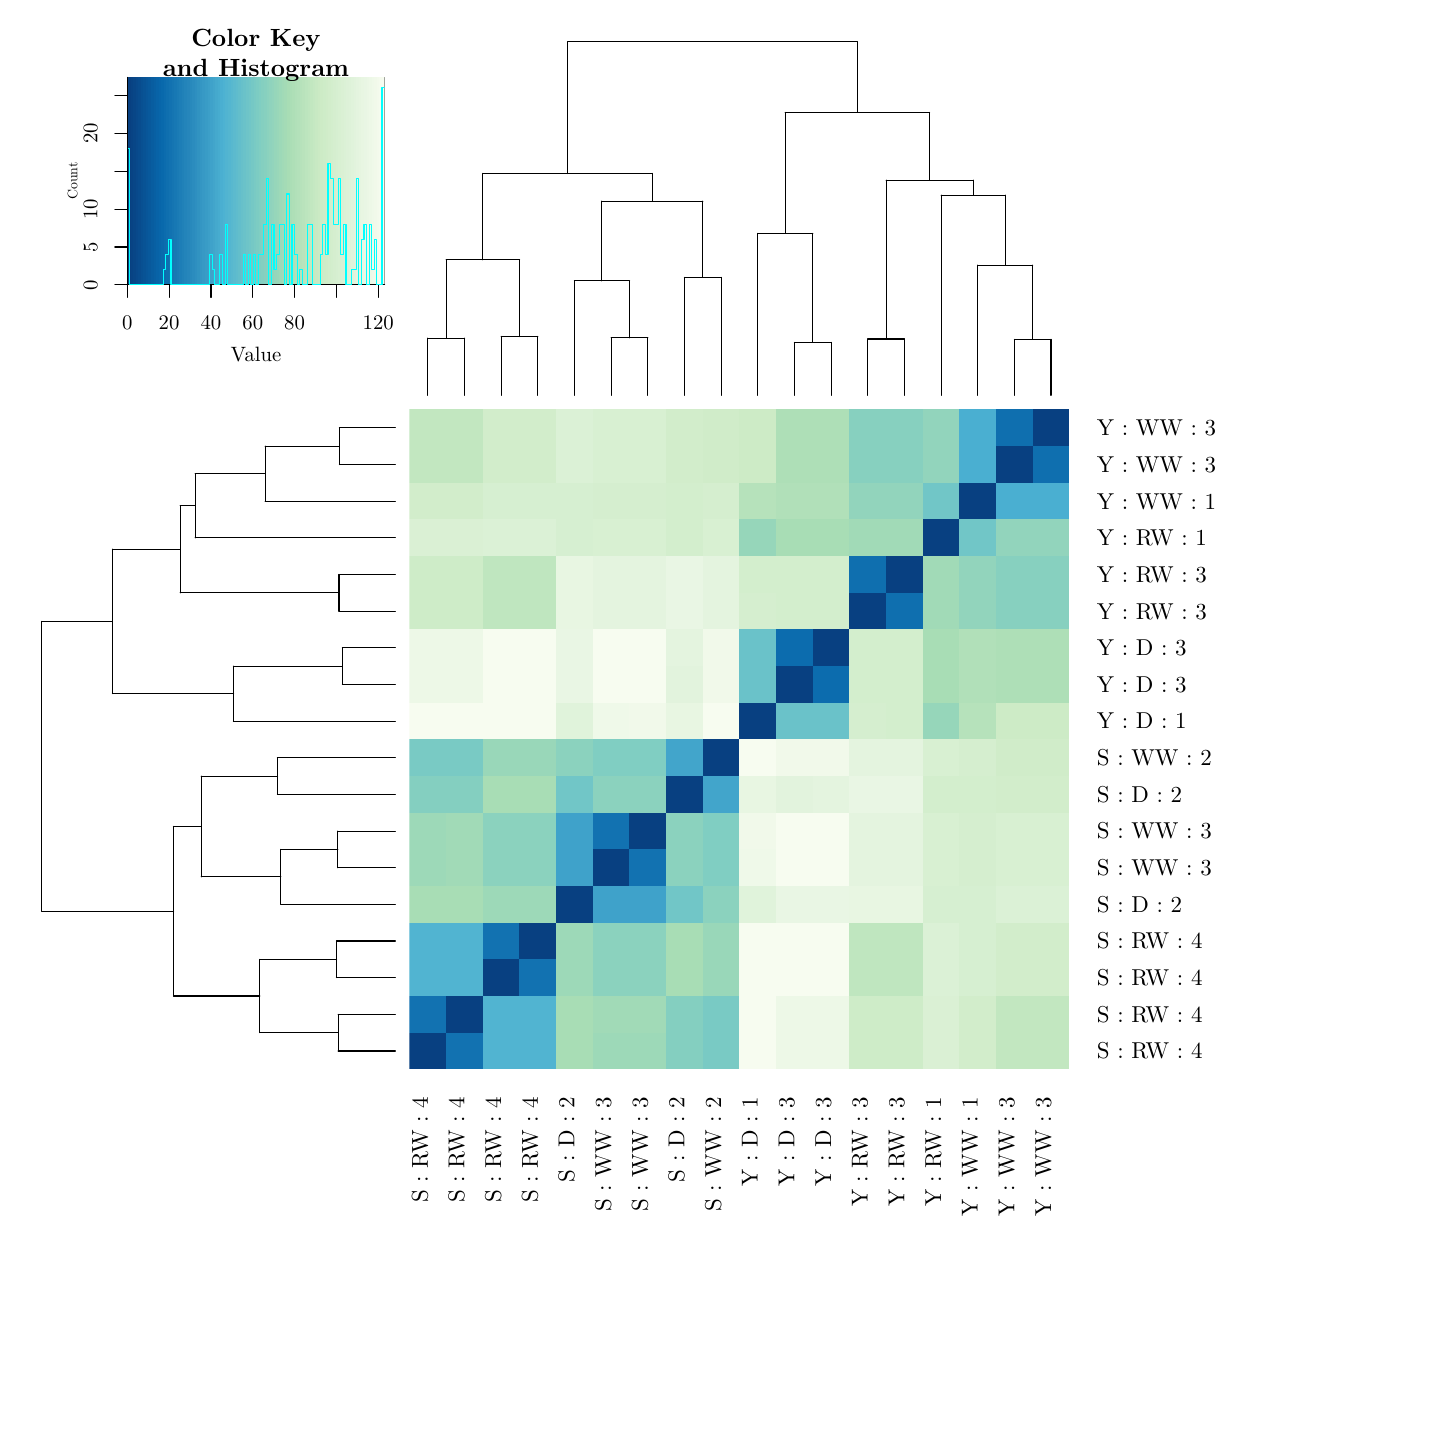
\begin{tikzpicture}[x=1pt,y=1pt]
\definecolor{fillColor}{RGB}{255,255,255}
\path[use as bounding box,fill=fillColor,fill opacity=0.00] (0,0) rectangle (505.89,505.89);
\begin{scope}
\path[clip] (137.97,129.48) rectangle (376.41,367.92);
\definecolor{fillColor}{RGB}{8,64,129}

\path[fill=fillColor] (137.97,129.48) rectangle (151.22,142.73);
\definecolor{fillColor}{RGB}{18,114,177}

\path[fill=fillColor] (137.97,142.73) rectangle (151.22,155.97);
\definecolor{fillColor}{RGB}{81,180,209}

\path[fill=fillColor] (137.97,155.97) rectangle (151.22,169.22);

\path[fill=fillColor] (137.97,169.22) rectangle (151.22,182.47);
\definecolor{fillColor}{RGB}{168,221,181}

\path[fill=fillColor] (137.97,182.47) rectangle (151.22,195.71);
\definecolor{fillColor}{RGB}{157,217,184}

\path[fill=fillColor] (137.97,195.71) rectangle (151.22,208.96);

\path[fill=fillColor] (137.97,208.96) rectangle (151.22,222.21);
\definecolor{fillColor}{RGB}{132,207,192}

\path[fill=fillColor] (137.97,222.21) rectangle (151.22,235.45);
\definecolor{fillColor}{RGB}{121,202,196}

\path[fill=fillColor] (137.97,235.45) rectangle (151.22,248.70);
\definecolor{fillColor}{RGB}{247,252,240}

\path[fill=fillColor] (137.97,248.70) rectangle (151.22,261.95);
\definecolor{fillColor}{RGB}{237,248,231}

\path[fill=fillColor] (137.97,261.95) rectangle (151.22,275.19);

\path[fill=fillColor] (137.97,275.19) rectangle (151.22,288.44);
\definecolor{fillColor}{RGB}{206,236,200}

\path[fill=fillColor] (137.97,288.44) rectangle (151.22,301.69);

\path[fill=fillColor] (137.97,301.69) rectangle (151.22,314.93);
\definecolor{fillColor}{RGB}{218,240,212}

\path[fill=fillColor] (137.97,314.93) rectangle (151.22,328.18);
\definecolor{fillColor}{RGB}{210,237,203}

\path[fill=fillColor] (137.97,328.18) rectangle (151.22,341.43);
\definecolor{fillColor}{RGB}{194,231,192}

\path[fill=fillColor] (137.97,341.43) rectangle (151.22,354.67);

\path[fill=fillColor] (137.97,354.67) rectangle (151.22,367.92);
\definecolor{fillColor}{RGB}{18,114,177}

\path[fill=fillColor] (151.22,129.48) rectangle (164.46,142.73);
\definecolor{fillColor}{RGB}{8,64,129}

\path[fill=fillColor] (151.22,142.73) rectangle (164.46,155.97);
\definecolor{fillColor}{RGB}{81,180,209}

\path[fill=fillColor] (151.22,155.97) rectangle (164.46,169.22);

\path[fill=fillColor] (151.22,169.22) rectangle (164.46,182.47);
\definecolor{fillColor}{RGB}{168,221,181}

\path[fill=fillColor] (151.22,182.47) rectangle (164.46,195.71);
\definecolor{fillColor}{RGB}{161,218,183}

\path[fill=fillColor] (151.22,195.71) rectangle (164.46,208.96);

\path[fill=fillColor] (151.22,208.96) rectangle (164.46,222.21);
\definecolor{fillColor}{RGB}{132,207,192}

\path[fill=fillColor] (151.22,222.21) rectangle (164.46,235.45);
\definecolor{fillColor}{RGB}{121,202,196}

\path[fill=fillColor] (151.22,235.45) rectangle (164.46,248.70);
\definecolor{fillColor}{RGB}{247,252,240}

\path[fill=fillColor] (151.22,248.70) rectangle (164.46,261.95);
\definecolor{fillColor}{RGB}{237,248,231}

\path[fill=fillColor] (151.22,261.95) rectangle (164.46,275.19);

\path[fill=fillColor] (151.22,275.19) rectangle (164.46,288.44);
\definecolor{fillColor}{RGB}{206,236,200}

\path[fill=fillColor] (151.22,288.44) rectangle (164.46,301.69);

\path[fill=fillColor] (151.22,301.69) rectangle (164.46,314.93);
\definecolor{fillColor}{RGB}{218,240,212}

\path[fill=fillColor] (151.22,314.93) rectangle (164.46,328.18);
\definecolor{fillColor}{RGB}{210,237,203}

\path[fill=fillColor] (151.22,328.18) rectangle (164.46,341.43);
\definecolor{fillColor}{RGB}{194,231,192}

\path[fill=fillColor] (151.22,341.43) rectangle (164.46,354.67);

\path[fill=fillColor] (151.22,354.67) rectangle (164.46,367.92);
\definecolor{fillColor}{RGB}{81,180,209}

\path[fill=fillColor] (164.46,129.48) rectangle (177.71,142.73);

\path[fill=fillColor] (164.46,142.73) rectangle (177.71,155.97);
\definecolor{fillColor}{RGB}{8,64,129}

\path[fill=fillColor] (164.46,155.97) rectangle (177.71,169.22);
\definecolor{fillColor}{RGB}{18,114,177}

\path[fill=fillColor] (164.46,169.22) rectangle (177.71,182.47);
\definecolor{fillColor}{RGB}{157,217,184}

\path[fill=fillColor] (164.46,182.47) rectangle (177.71,195.71);
\definecolor{fillColor}{RGB}{139,210,190}

\path[fill=fillColor] (164.46,195.71) rectangle (177.71,208.96);

\path[fill=fillColor] (164.46,208.96) rectangle (177.71,222.21);
\definecolor{fillColor}{RGB}{168,221,181}

\path[fill=fillColor] (164.46,222.21) rectangle (177.71,235.45);
\definecolor{fillColor}{RGB}{153,215,185}

\path[fill=fillColor] (164.46,235.45) rectangle (177.71,248.70);
\definecolor{fillColor}{RGB}{247,252,240}

\path[fill=fillColor] (164.46,248.70) rectangle (177.71,261.95);

\path[fill=fillColor] (164.46,261.95) rectangle (177.71,275.19);

\path[fill=fillColor] (164.46,275.19) rectangle (177.71,288.44);
\definecolor{fillColor}{RGB}{191,230,191}

\path[fill=fillColor] (164.46,288.44) rectangle (177.71,301.69);

\path[fill=fillColor] (164.46,301.69) rectangle (177.71,314.93);
\definecolor{fillColor}{RGB}{219,241,214}

\path[fill=fillColor] (164.46,314.93) rectangle (177.71,328.18);
\definecolor{fillColor}{RGB}{214,239,209}

\path[fill=fillColor] (164.46,328.18) rectangle (177.71,341.43);
\definecolor{fillColor}{RGB}{210,237,203}

\path[fill=fillColor] (164.46,341.43) rectangle (177.71,354.67);

\path[fill=fillColor] (164.46,354.67) rectangle (177.71,367.92);
\definecolor{fillColor}{RGB}{81,180,209}

\path[fill=fillColor] (177.71,129.48) rectangle (190.96,142.73);

\path[fill=fillColor] (177.71,142.73) rectangle (190.96,155.97);
\definecolor{fillColor}{RGB}{18,114,177}

\path[fill=fillColor] (177.71,155.97) rectangle (190.96,169.22);
\definecolor{fillColor}{RGB}{8,64,129}

\path[fill=fillColor] (177.71,169.22) rectangle (190.96,182.47);
\definecolor{fillColor}{RGB}{157,217,184}

\path[fill=fillColor] (177.71,182.47) rectangle (190.96,195.71);
\definecolor{fillColor}{RGB}{139,210,190}

\path[fill=fillColor] (177.71,195.71) rectangle (190.96,208.96);

\path[fill=fillColor] (177.71,208.96) rectangle (190.96,222.21);
\definecolor{fillColor}{RGB}{168,221,181}

\path[fill=fillColor] (177.71,222.21) rectangle (190.96,235.45);
\definecolor{fillColor}{RGB}{153,215,185}

\path[fill=fillColor] (177.71,235.45) rectangle (190.96,248.70);
\definecolor{fillColor}{RGB}{247,252,240}

\path[fill=fillColor] (177.71,248.70) rectangle (190.96,261.95);

\path[fill=fillColor] (177.71,261.95) rectangle (190.96,275.19);

\path[fill=fillColor] (177.71,275.19) rectangle (190.96,288.44);
\definecolor{fillColor}{RGB}{191,230,191}

\path[fill=fillColor] (177.71,288.44) rectangle (190.96,301.69);

\path[fill=fillColor] (177.71,301.69) rectangle (190.96,314.93);
\definecolor{fillColor}{RGB}{219,241,214}

\path[fill=fillColor] (177.71,314.93) rectangle (190.96,328.18);
\definecolor{fillColor}{RGB}{214,239,209}

\path[fill=fillColor] (177.71,328.18) rectangle (190.96,341.43);
\definecolor{fillColor}{RGB}{210,237,203}

\path[fill=fillColor] (177.71,341.43) rectangle (190.96,354.67);

\path[fill=fillColor] (177.71,354.67) rectangle (190.96,367.92);
\definecolor{fillColor}{RGB}{168,221,181}

\path[fill=fillColor] (190.96,129.48) rectangle (204.20,142.73);

\path[fill=fillColor] (190.96,142.73) rectangle (204.20,155.97);
\definecolor{fillColor}{RGB}{157,217,184}

\path[fill=fillColor] (190.96,155.97) rectangle (204.20,169.22);

\path[fill=fillColor] (190.96,169.22) rectangle (204.20,182.47);
\definecolor{fillColor}{RGB}{8,64,129}

\path[fill=fillColor] (190.96,182.47) rectangle (204.20,195.71);
\definecolor{fillColor}{RGB}{63,162,202}

\path[fill=fillColor] (190.96,195.71) rectangle (204.20,208.96);

\path[fill=fillColor] (190.96,208.96) rectangle (204.20,222.21);
\definecolor{fillColor}{RGB}{113,198,199}

\path[fill=fillColor] (190.96,222.21) rectangle (204.20,235.45);
\definecolor{fillColor}{RGB}{139,210,190}

\path[fill=fillColor] (190.96,235.45) rectangle (204.20,248.70);
\definecolor{fillColor}{RGB}{224,243,219}

\path[fill=fillColor] (190.96,248.70) rectangle (204.20,261.95);
\definecolor{fillColor}{RGB}{233,246,228}

\path[fill=fillColor] (190.96,261.95) rectangle (204.20,275.19);

\path[fill=fillColor] (190.96,275.19) rectangle (204.20,288.44);
\definecolor{fillColor}{RGB}{232,246,226}

\path[fill=fillColor] (190.96,288.44) rectangle (204.20,301.69);

\path[fill=fillColor] (190.96,301.69) rectangle (204.20,314.93);
\definecolor{fillColor}{RGB}{214,239,209}

\path[fill=fillColor] (190.96,314.93) rectangle (204.20,328.18);

\path[fill=fillColor] (190.96,328.18) rectangle (204.20,341.43);
\definecolor{fillColor}{RGB}{219,241,214}

\path[fill=fillColor] (190.96,341.43) rectangle (204.20,354.67);

\path[fill=fillColor] (190.96,354.67) rectangle (204.20,367.92);
\definecolor{fillColor}{RGB}{157,217,184}

\path[fill=fillColor] (204.20,129.48) rectangle (217.45,142.73);
\definecolor{fillColor}{RGB}{161,218,183}

\path[fill=fillColor] (204.20,142.73) rectangle (217.45,155.97);
\definecolor{fillColor}{RGB}{139,210,190}

\path[fill=fillColor] (204.20,155.97) rectangle (217.45,169.22);

\path[fill=fillColor] (204.20,169.22) rectangle (217.45,182.47);
\definecolor{fillColor}{RGB}{63,162,202}

\path[fill=fillColor] (204.20,182.47) rectangle (217.45,195.71);
\definecolor{fillColor}{RGB}{8,64,129}

\path[fill=fillColor] (204.20,195.71) rectangle (217.45,208.96);
\definecolor{fillColor}{RGB}{18,114,177}

\path[fill=fillColor] (204.20,208.96) rectangle (217.45,222.21);
\definecolor{fillColor}{RGB}{139,210,190}

\path[fill=fillColor] (204.20,222.21) rectangle (217.45,235.45);
\definecolor{fillColor}{RGB}{128,206,194}

\path[fill=fillColor] (204.20,235.45) rectangle (217.45,248.70);
\definecolor{fillColor}{RGB}{239,249,233}

\path[fill=fillColor] (204.20,248.70) rectangle (217.45,261.95);
\definecolor{fillColor}{RGB}{247,252,240}

\path[fill=fillColor] (204.20,261.95) rectangle (217.45,275.19);

\path[fill=fillColor] (204.20,275.19) rectangle (217.45,288.44);
\definecolor{fillColor}{RGB}{228,244,223}

\path[fill=fillColor] (204.20,288.44) rectangle (217.45,301.69);

\path[fill=fillColor] (204.20,301.69) rectangle (217.45,314.93);
\definecolor{fillColor}{RGB}{216,240,210}

\path[fill=fillColor] (204.20,314.93) rectangle (217.45,328.18);
\definecolor{fillColor}{RGB}{213,238,207}

\path[fill=fillColor] (204.20,328.18) rectangle (217.45,341.43);
\definecolor{fillColor}{RGB}{216,240,210}

\path[fill=fillColor] (204.20,341.43) rectangle (217.45,354.67);

\path[fill=fillColor] (204.20,354.67) rectangle (217.45,367.92);
\definecolor{fillColor}{RGB}{157,217,184}

\path[fill=fillColor] (217.45,129.48) rectangle (230.70,142.73);
\definecolor{fillColor}{RGB}{161,218,183}

\path[fill=fillColor] (217.45,142.73) rectangle (230.70,155.97);
\definecolor{fillColor}{RGB}{139,210,190}

\path[fill=fillColor] (217.45,155.97) rectangle (230.70,169.22);

\path[fill=fillColor] (217.45,169.22) rectangle (230.70,182.47);
\definecolor{fillColor}{RGB}{63,162,202}

\path[fill=fillColor] (217.45,182.47) rectangle (230.70,195.71);
\definecolor{fillColor}{RGB}{18,114,177}

\path[fill=fillColor] (217.45,195.71) rectangle (230.70,208.96);
\definecolor{fillColor}{RGB}{8,64,129}

\path[fill=fillColor] (217.45,208.96) rectangle (230.70,222.21);
\definecolor{fillColor}{RGB}{139,210,190}

\path[fill=fillColor] (217.45,222.21) rectangle (230.70,235.45);
\definecolor{fillColor}{RGB}{128,206,194}

\path[fill=fillColor] (217.45,235.45) rectangle (230.70,248.70);
\definecolor{fillColor}{RGB}{241,249,234}

\path[fill=fillColor] (217.45,248.70) rectangle (230.70,261.95);
\definecolor{fillColor}{RGB}{247,252,240}

\path[fill=fillColor] (217.45,261.95) rectangle (230.70,275.19);

\path[fill=fillColor] (217.45,275.19) rectangle (230.70,288.44);
\definecolor{fillColor}{RGB}{228,244,223}

\path[fill=fillColor] (217.45,288.44) rectangle (230.70,301.69);

\path[fill=fillColor] (217.45,301.69) rectangle (230.70,314.93);
\definecolor{fillColor}{RGB}{216,240,210}

\path[fill=fillColor] (217.45,314.93) rectangle (230.70,328.18);
\definecolor{fillColor}{RGB}{213,238,207}

\path[fill=fillColor] (217.45,328.18) rectangle (230.70,341.43);
\definecolor{fillColor}{RGB}{216,240,210}

\path[fill=fillColor] (217.45,341.43) rectangle (230.70,354.67);

\path[fill=fillColor] (217.45,354.67) rectangle (230.70,367.92);
\definecolor{fillColor}{RGB}{132,207,192}

\path[fill=fillColor] (230.70,129.48) rectangle (243.94,142.73);

\path[fill=fillColor] (230.70,142.73) rectangle (243.94,155.97);
\definecolor{fillColor}{RGB}{168,221,181}

\path[fill=fillColor] (230.70,155.97) rectangle (243.94,169.22);

\path[fill=fillColor] (230.70,169.22) rectangle (243.94,182.47);
\definecolor{fillColor}{RGB}{113,198,199}

\path[fill=fillColor] (230.70,182.47) rectangle (243.94,195.71);
\definecolor{fillColor}{RGB}{139,210,190}

\path[fill=fillColor] (230.70,195.71) rectangle (243.94,208.96);

\path[fill=fillColor] (230.70,208.96) rectangle (243.94,222.21);
\definecolor{fillColor}{RGB}{8,64,129}

\path[fill=fillColor] (230.70,222.21) rectangle (243.94,235.45);
\definecolor{fillColor}{RGB}{66,165,203}

\path[fill=fillColor] (230.70,235.45) rectangle (243.94,248.70);
\definecolor{fillColor}{RGB}{232,246,226}

\path[fill=fillColor] (230.70,248.70) rectangle (243.94,261.95);
\definecolor{fillColor}{RGB}{226,243,221}

\path[fill=fillColor] (230.70,261.95) rectangle (243.94,275.19);
\definecolor{fillColor}{RGB}{228,244,223}

\path[fill=fillColor] (230.70,275.19) rectangle (243.94,288.44);
\definecolor{fillColor}{RGB}{233,246,228}

\path[fill=fillColor] (230.70,288.44) rectangle (243.94,301.69);

\path[fill=fillColor] (230.70,301.69) rectangle (243.94,314.93);
\definecolor{fillColor}{RGB}{211,238,205}

\path[fill=fillColor] (230.70,314.93) rectangle (243.94,328.18);

\path[fill=fillColor] (230.70,328.18) rectangle (243.94,341.43);
\definecolor{fillColor}{RGB}{210,237,203}

\path[fill=fillColor] (230.70,341.43) rectangle (243.94,354.67);

\path[fill=fillColor] (230.70,354.67) rectangle (243.94,367.92);
\definecolor{fillColor}{RGB}{121,202,196}

\path[fill=fillColor] (243.94,129.48) rectangle (257.19,142.73);

\path[fill=fillColor] (243.94,142.73) rectangle (257.19,155.97);
\definecolor{fillColor}{RGB}{153,215,185}

\path[fill=fillColor] (243.94,155.97) rectangle (257.19,169.22);

\path[fill=fillColor] (243.94,169.22) rectangle (257.19,182.47);
\definecolor{fillColor}{RGB}{139,210,190}

\path[fill=fillColor] (243.94,182.47) rectangle (257.19,195.71);
\definecolor{fillColor}{RGB}{128,206,194}

\path[fill=fillColor] (243.94,195.71) rectangle (257.19,208.96);

\path[fill=fillColor] (243.94,208.96) rectangle (257.19,222.21);
\definecolor{fillColor}{RGB}{66,165,203}

\path[fill=fillColor] (243.94,222.21) rectangle (257.19,235.45);
\definecolor{fillColor}{RGB}{8,64,129}

\path[fill=fillColor] (243.94,235.45) rectangle (257.19,248.70);
\definecolor{fillColor}{RGB}{247,252,240}

\path[fill=fillColor] (243.94,248.70) rectangle (257.19,261.95);
\definecolor{fillColor}{RGB}{241,249,234}

\path[fill=fillColor] (243.94,261.95) rectangle (257.19,275.19);

\path[fill=fillColor] (243.94,275.19) rectangle (257.19,288.44);
\definecolor{fillColor}{RGB}{228,244,223}

\path[fill=fillColor] (243.94,288.44) rectangle (257.19,301.69);

\path[fill=fillColor] (243.94,301.69) rectangle (257.19,314.93);
\definecolor{fillColor}{RGB}{216,240,210}

\path[fill=fillColor] (243.94,314.93) rectangle (257.19,328.18);
\definecolor{fillColor}{RGB}{213,238,207}

\path[fill=fillColor] (243.94,328.18) rectangle (257.19,341.43);
\definecolor{fillColor}{RGB}{208,236,201}

\path[fill=fillColor] (243.94,341.43) rectangle (257.19,354.67);

\path[fill=fillColor] (243.94,354.67) rectangle (257.19,367.92);
\definecolor{fillColor}{RGB}{247,252,240}

\path[fill=fillColor] (257.19,129.48) rectangle (270.44,142.73);

\path[fill=fillColor] (257.19,142.73) rectangle (270.44,155.97);

\path[fill=fillColor] (257.19,155.97) rectangle (270.44,169.22);

\path[fill=fillColor] (257.19,169.22) rectangle (270.44,182.47);
\definecolor{fillColor}{RGB}{224,243,219}

\path[fill=fillColor] (257.19,182.47) rectangle (270.44,195.71);
\definecolor{fillColor}{RGB}{239,249,233}

\path[fill=fillColor] (257.19,195.71) rectangle (270.44,208.96);
\definecolor{fillColor}{RGB}{241,249,234}

\path[fill=fillColor] (257.19,208.96) rectangle (270.44,222.21);
\definecolor{fillColor}{RGB}{232,246,226}

\path[fill=fillColor] (257.19,222.21) rectangle (270.44,235.45);
\definecolor{fillColor}{RGB}{247,252,240}

\path[fill=fillColor] (257.19,235.45) rectangle (270.44,248.70);
\definecolor{fillColor}{RGB}{8,64,129}

\path[fill=fillColor] (257.19,248.70) rectangle (270.44,261.95);
\definecolor{fillColor}{RGB}{106,194,201}

\path[fill=fillColor] (257.19,261.95) rectangle (270.44,275.19);

\path[fill=fillColor] (257.19,275.19) rectangle (270.44,288.44);
\definecolor{fillColor}{RGB}{213,238,207}

\path[fill=fillColor] (257.19,288.44) rectangle (270.44,301.69);
\definecolor{fillColor}{RGB}{211,238,205}

\path[fill=fillColor] (257.19,301.69) rectangle (270.44,314.93);
\definecolor{fillColor}{RGB}{150,214,186}

\path[fill=fillColor] (257.19,314.93) rectangle (270.44,328.18);
\definecolor{fillColor}{RGB}{182,226,187}

\path[fill=fillColor] (257.19,328.18) rectangle (270.44,341.43);
\definecolor{fillColor}{RGB}{205,235,198}

\path[fill=fillColor] (257.19,341.43) rectangle (270.44,354.67);

\path[fill=fillColor] (257.19,354.67) rectangle (270.44,367.92);
\definecolor{fillColor}{RGB}{237,248,231}

\path[fill=fillColor] (270.44,129.48) rectangle (283.68,142.73);

\path[fill=fillColor] (270.44,142.73) rectangle (283.68,155.97);
\definecolor{fillColor}{RGB}{247,252,240}

\path[fill=fillColor] (270.44,155.97) rectangle (283.68,169.22);

\path[fill=fillColor] (270.44,169.22) rectangle (283.68,182.47);
\definecolor{fillColor}{RGB}{233,246,228}

\path[fill=fillColor] (270.44,182.47) rectangle (283.68,195.71);
\definecolor{fillColor}{RGB}{247,252,240}

\path[fill=fillColor] (270.44,195.71) rectangle (283.68,208.96);

\path[fill=fillColor] (270.44,208.96) rectangle (283.68,222.21);
\definecolor{fillColor}{RGB}{226,243,221}

\path[fill=fillColor] (270.44,222.21) rectangle (283.68,235.45);
\definecolor{fillColor}{RGB}{241,249,234}

\path[fill=fillColor] (270.44,235.45) rectangle (283.68,248.70);
\definecolor{fillColor}{RGB}{106,194,201}

\path[fill=fillColor] (270.44,248.70) rectangle (283.68,261.95);
\definecolor{fillColor}{RGB}{8,64,129}

\path[fill=fillColor] (270.44,261.95) rectangle (283.68,275.19);
\definecolor{fillColor}{RGB}{12,108,174}

\path[fill=fillColor] (270.44,275.19) rectangle (283.68,288.44);
\definecolor{fillColor}{RGB}{211,238,205}

\path[fill=fillColor] (270.44,288.44) rectangle (283.68,301.69);

\path[fill=fillColor] (270.44,301.69) rectangle (283.68,314.93);
\definecolor{fillColor}{RGB}{168,221,181}

\path[fill=fillColor] (270.44,314.93) rectangle (283.68,328.18);
\definecolor{fillColor}{RGB}{177,224,185}

\path[fill=fillColor] (270.44,328.18) rectangle (283.68,341.43);
\definecolor{fillColor}{RGB}{174,223,183}

\path[fill=fillColor] (270.44,341.43) rectangle (283.68,354.67);

\path[fill=fillColor] (270.44,354.67) rectangle (283.68,367.92);
\definecolor{fillColor}{RGB}{237,248,231}

\path[fill=fillColor] (283.68,129.48) rectangle (296.93,142.73);

\path[fill=fillColor] (283.68,142.73) rectangle (296.93,155.97);
\definecolor{fillColor}{RGB}{247,252,240}

\path[fill=fillColor] (283.68,155.97) rectangle (296.93,169.22);

\path[fill=fillColor] (283.68,169.22) rectangle (296.93,182.47);
\definecolor{fillColor}{RGB}{233,246,228}

\path[fill=fillColor] (283.68,182.47) rectangle (296.93,195.71);
\definecolor{fillColor}{RGB}{247,252,240}

\path[fill=fillColor] (283.68,195.71) rectangle (296.93,208.96);

\path[fill=fillColor] (283.68,208.96) rectangle (296.93,222.21);
\definecolor{fillColor}{RGB}{228,244,223}

\path[fill=fillColor] (283.68,222.21) rectangle (296.93,235.45);
\definecolor{fillColor}{RGB}{241,249,234}

\path[fill=fillColor] (283.68,235.45) rectangle (296.93,248.70);
\definecolor{fillColor}{RGB}{106,194,201}

\path[fill=fillColor] (283.68,248.70) rectangle (296.93,261.95);
\definecolor{fillColor}{RGB}{12,108,174}

\path[fill=fillColor] (283.68,261.95) rectangle (296.93,275.19);
\definecolor{fillColor}{RGB}{8,64,129}

\path[fill=fillColor] (283.68,275.19) rectangle (296.93,288.44);
\definecolor{fillColor}{RGB}{211,238,205}

\path[fill=fillColor] (283.68,288.44) rectangle (296.93,301.69);

\path[fill=fillColor] (283.68,301.69) rectangle (296.93,314.93);
\definecolor{fillColor}{RGB}{168,221,181}

\path[fill=fillColor] (283.68,314.93) rectangle (296.93,328.18);
\definecolor{fillColor}{RGB}{177,224,185}

\path[fill=fillColor] (283.68,328.18) rectangle (296.93,341.43);
\definecolor{fillColor}{RGB}{174,223,183}

\path[fill=fillColor] (283.68,341.43) rectangle (296.93,354.67);

\path[fill=fillColor] (283.68,354.67) rectangle (296.93,367.92);
\definecolor{fillColor}{RGB}{206,236,200}

\path[fill=fillColor] (296.93,129.48) rectangle (310.18,142.73);

\path[fill=fillColor] (296.93,142.73) rectangle (310.18,155.97);
\definecolor{fillColor}{RGB}{191,230,191}

\path[fill=fillColor] (296.93,155.97) rectangle (310.18,169.22);

\path[fill=fillColor] (296.93,169.22) rectangle (310.18,182.47);
\definecolor{fillColor}{RGB}{232,246,226}

\path[fill=fillColor] (296.93,182.47) rectangle (310.18,195.71);
\definecolor{fillColor}{RGB}{228,244,223}

\path[fill=fillColor] (296.93,195.71) rectangle (310.18,208.96);

\path[fill=fillColor] (296.93,208.96) rectangle (310.18,222.21);
\definecolor{fillColor}{RGB}{233,246,228}

\path[fill=fillColor] (296.93,222.21) rectangle (310.18,235.45);
\definecolor{fillColor}{RGB}{228,244,223}

\path[fill=fillColor] (296.93,235.45) rectangle (310.18,248.70);
\definecolor{fillColor}{RGB}{213,238,207}

\path[fill=fillColor] (296.93,248.70) rectangle (310.18,261.95);
\definecolor{fillColor}{RGB}{211,238,205}

\path[fill=fillColor] (296.93,261.95) rectangle (310.18,275.19);

\path[fill=fillColor] (296.93,275.19) rectangle (310.18,288.44);
\definecolor{fillColor}{RGB}{8,64,129}

\path[fill=fillColor] (296.93,288.44) rectangle (310.18,301.69);
\definecolor{fillColor}{RGB}{15,111,175}

\path[fill=fillColor] (296.93,301.69) rectangle (310.18,314.93);
\definecolor{fillColor}{RGB}{161,218,183}

\path[fill=fillColor] (296.93,314.93) rectangle (310.18,328.18);
\definecolor{fillColor}{RGB}{146,212,188}

\path[fill=fillColor] (296.93,328.18) rectangle (310.18,341.43);
\definecolor{fillColor}{RGB}{135,208,191}

\path[fill=fillColor] (296.93,341.43) rectangle (310.18,354.67);

\path[fill=fillColor] (296.93,354.67) rectangle (310.18,367.92);
\definecolor{fillColor}{RGB}{206,236,200}

\path[fill=fillColor] (310.18,129.48) rectangle (323.42,142.73);

\path[fill=fillColor] (310.18,142.73) rectangle (323.42,155.97);
\definecolor{fillColor}{RGB}{191,230,191}

\path[fill=fillColor] (310.18,155.97) rectangle (323.42,169.22);

\path[fill=fillColor] (310.18,169.22) rectangle (323.42,182.47);
\definecolor{fillColor}{RGB}{232,246,226}

\path[fill=fillColor] (310.18,182.47) rectangle (323.42,195.71);
\definecolor{fillColor}{RGB}{228,244,223}

\path[fill=fillColor] (310.18,195.71) rectangle (323.42,208.96);

\path[fill=fillColor] (310.18,208.96) rectangle (323.42,222.21);
\definecolor{fillColor}{RGB}{233,246,228}

\path[fill=fillColor] (310.18,222.21) rectangle (323.42,235.45);
\definecolor{fillColor}{RGB}{228,244,223}

\path[fill=fillColor] (310.18,235.45) rectangle (323.42,248.70);
\definecolor{fillColor}{RGB}{211,238,205}

\path[fill=fillColor] (310.18,248.70) rectangle (323.42,261.95);

\path[fill=fillColor] (310.18,261.95) rectangle (323.42,275.19);

\path[fill=fillColor] (310.18,275.19) rectangle (323.42,288.44);
\definecolor{fillColor}{RGB}{15,111,175}

\path[fill=fillColor] (310.18,288.44) rectangle (323.42,301.69);
\definecolor{fillColor}{RGB}{8,64,129}

\path[fill=fillColor] (310.18,301.69) rectangle (323.42,314.93);
\definecolor{fillColor}{RGB}{161,218,183}

\path[fill=fillColor] (310.18,314.93) rectangle (323.42,328.18);
\definecolor{fillColor}{RGB}{146,212,188}

\path[fill=fillColor] (310.18,328.18) rectangle (323.42,341.43);
\definecolor{fillColor}{RGB}{135,208,191}

\path[fill=fillColor] (310.18,341.43) rectangle (323.42,354.67);

\path[fill=fillColor] (310.18,354.67) rectangle (323.42,367.92);
\definecolor{fillColor}{RGB}{218,240,212}

\path[fill=fillColor] (323.42,129.48) rectangle (336.67,142.73);

\path[fill=fillColor] (323.42,142.73) rectangle (336.67,155.97);
\definecolor{fillColor}{RGB}{219,241,214}

\path[fill=fillColor] (323.42,155.97) rectangle (336.67,169.22);

\path[fill=fillColor] (323.42,169.22) rectangle (336.67,182.47);
\definecolor{fillColor}{RGB}{214,239,209}

\path[fill=fillColor] (323.42,182.47) rectangle (336.67,195.71);
\definecolor{fillColor}{RGB}{216,240,210}

\path[fill=fillColor] (323.42,195.71) rectangle (336.67,208.96);

\path[fill=fillColor] (323.42,208.96) rectangle (336.67,222.21);
\definecolor{fillColor}{RGB}{211,238,205}

\path[fill=fillColor] (323.42,222.21) rectangle (336.67,235.45);
\definecolor{fillColor}{RGB}{216,240,210}

\path[fill=fillColor] (323.42,235.45) rectangle (336.67,248.70);
\definecolor{fillColor}{RGB}{150,214,186}

\path[fill=fillColor] (323.42,248.70) rectangle (336.67,261.95);
\definecolor{fillColor}{RGB}{168,221,181}

\path[fill=fillColor] (323.42,261.95) rectangle (336.67,275.19);

\path[fill=fillColor] (323.42,275.19) rectangle (336.67,288.44);
\definecolor{fillColor}{RGB}{161,218,183}

\path[fill=fillColor] (323.42,288.44) rectangle (336.67,301.69);

\path[fill=fillColor] (323.42,301.69) rectangle (336.67,314.93);
\definecolor{fillColor}{RGB}{8,64,129}

\path[fill=fillColor] (323.42,314.93) rectangle (336.67,328.18);
\definecolor{fillColor}{RGB}{113,198,199}

\path[fill=fillColor] (323.42,328.18) rectangle (336.67,341.43);
\definecolor{fillColor}{RGB}{146,212,188}

\path[fill=fillColor] (323.42,341.43) rectangle (336.67,354.67);

\path[fill=fillColor] (323.42,354.67) rectangle (336.67,367.92);
\definecolor{fillColor}{RGB}{210,237,203}

\path[fill=fillColor] (336.67,129.48) rectangle (349.92,142.73);

\path[fill=fillColor] (336.67,142.73) rectangle (349.92,155.97);
\definecolor{fillColor}{RGB}{214,239,209}

\path[fill=fillColor] (336.67,155.97) rectangle (349.92,169.22);

\path[fill=fillColor] (336.67,169.22) rectangle (349.92,182.47);

\path[fill=fillColor] (336.67,182.47) rectangle (349.92,195.71);
\definecolor{fillColor}{RGB}{213,238,207}

\path[fill=fillColor] (336.67,195.71) rectangle (349.92,208.96);

\path[fill=fillColor] (336.67,208.96) rectangle (349.92,222.21);
\definecolor{fillColor}{RGB}{211,238,205}

\path[fill=fillColor] (336.67,222.21) rectangle (349.92,235.45);
\definecolor{fillColor}{RGB}{213,238,207}

\path[fill=fillColor] (336.67,235.45) rectangle (349.92,248.70);
\definecolor{fillColor}{RGB}{182,226,187}

\path[fill=fillColor] (336.67,248.70) rectangle (349.92,261.95);
\definecolor{fillColor}{RGB}{177,224,185}

\path[fill=fillColor] (336.67,261.95) rectangle (349.92,275.19);

\path[fill=fillColor] (336.67,275.19) rectangle (349.92,288.44);
\definecolor{fillColor}{RGB}{146,212,188}

\path[fill=fillColor] (336.67,288.44) rectangle (349.92,301.69);

\path[fill=fillColor] (336.67,301.69) rectangle (349.92,314.93);
\definecolor{fillColor}{RGB}{113,198,199}

\path[fill=fillColor] (336.67,314.93) rectangle (349.92,328.18);
\definecolor{fillColor}{RGB}{8,64,129}

\path[fill=fillColor] (336.67,328.18) rectangle (349.92,341.43);
\definecolor{fillColor}{RGB}{74,175,209}

\path[fill=fillColor] (336.67,341.43) rectangle (349.92,354.67);

\path[fill=fillColor] (336.67,354.67) rectangle (349.92,367.92);
\definecolor{fillColor}{RGB}{194,231,192}

\path[fill=fillColor] (349.92,129.48) rectangle (363.16,142.73);

\path[fill=fillColor] (349.92,142.73) rectangle (363.16,155.97);
\definecolor{fillColor}{RGB}{210,237,203}

\path[fill=fillColor] (349.92,155.97) rectangle (363.16,169.22);

\path[fill=fillColor] (349.92,169.22) rectangle (363.16,182.47);
\definecolor{fillColor}{RGB}{219,241,214}

\path[fill=fillColor] (349.92,182.47) rectangle (363.16,195.71);
\definecolor{fillColor}{RGB}{216,240,210}

\path[fill=fillColor] (349.92,195.71) rectangle (363.16,208.96);

\path[fill=fillColor] (349.92,208.96) rectangle (363.16,222.21);
\definecolor{fillColor}{RGB}{210,237,203}

\path[fill=fillColor] (349.92,222.21) rectangle (363.16,235.45);
\definecolor{fillColor}{RGB}{208,236,201}

\path[fill=fillColor] (349.92,235.45) rectangle (363.16,248.70);
\definecolor{fillColor}{RGB}{205,235,198}

\path[fill=fillColor] (349.92,248.70) rectangle (363.16,261.95);
\definecolor{fillColor}{RGB}{174,223,183}

\path[fill=fillColor] (349.92,261.95) rectangle (363.16,275.19);

\path[fill=fillColor] (349.92,275.19) rectangle (363.16,288.44);
\definecolor{fillColor}{RGB}{135,208,191}

\path[fill=fillColor] (349.92,288.44) rectangle (363.16,301.69);

\path[fill=fillColor] (349.92,301.69) rectangle (363.16,314.93);
\definecolor{fillColor}{RGB}{146,212,188}

\path[fill=fillColor] (349.92,314.93) rectangle (363.16,328.18);
\definecolor{fillColor}{RGB}{74,175,209}

\path[fill=fillColor] (349.92,328.18) rectangle (363.16,341.43);
\definecolor{fillColor}{RGB}{8,64,129}

\path[fill=fillColor] (349.92,341.43) rectangle (363.16,354.67);
\definecolor{fillColor}{RGB}{15,111,175}

\path[fill=fillColor] (349.92,354.67) rectangle (363.16,367.92);
\definecolor{fillColor}{RGB}{194,231,192}

\path[fill=fillColor] (363.16,129.48) rectangle (376.41,142.73);

\path[fill=fillColor] (363.16,142.73) rectangle (376.41,155.97);
\definecolor{fillColor}{RGB}{210,237,203}

\path[fill=fillColor] (363.16,155.97) rectangle (376.41,169.22);

\path[fill=fillColor] (363.16,169.22) rectangle (376.41,182.47);
\definecolor{fillColor}{RGB}{219,241,214}

\path[fill=fillColor] (363.16,182.47) rectangle (376.41,195.71);
\definecolor{fillColor}{RGB}{216,240,210}

\path[fill=fillColor] (363.16,195.71) rectangle (376.41,208.96);

\path[fill=fillColor] (363.16,208.96) rectangle (376.41,222.21);
\definecolor{fillColor}{RGB}{210,237,203}

\path[fill=fillColor] (363.16,222.21) rectangle (376.41,235.45);
\definecolor{fillColor}{RGB}{208,236,201}

\path[fill=fillColor] (363.16,235.45) rectangle (376.41,248.70);
\definecolor{fillColor}{RGB}{205,235,198}

\path[fill=fillColor] (363.16,248.70) rectangle (376.41,261.95);
\definecolor{fillColor}{RGB}{174,223,183}

\path[fill=fillColor] (363.16,261.95) rectangle (376.41,275.19);

\path[fill=fillColor] (363.16,275.19) rectangle (376.41,288.44);
\definecolor{fillColor}{RGB}{135,208,191}

\path[fill=fillColor] (363.16,288.44) rectangle (376.41,301.69);

\path[fill=fillColor] (363.16,301.69) rectangle (376.41,314.93);
\definecolor{fillColor}{RGB}{146,212,188}

\path[fill=fillColor] (363.16,314.93) rectangle (376.41,328.18);
\definecolor{fillColor}{RGB}{74,175,209}

\path[fill=fillColor] (363.16,328.18) rectangle (376.41,341.43);
\definecolor{fillColor}{RGB}{15,111,175}

\path[fill=fillColor] (363.16,341.43) rectangle (376.41,354.67);
\definecolor{fillColor}{RGB}{8,64,129}

\path[fill=fillColor] (363.16,354.67) rectangle (376.41,367.92);
\end{scope}
\begin{scope}
\path[clip] (  0.00,  0.00) rectangle (505.89,505.89);
\definecolor{drawColor}{RGB}{0,0,0}

\node[text=drawColor,rotate= 90.00,anchor=base east,inner sep=0pt, outer sep=0pt, scale=  0.83] at (144.59,119.52) {S : RW : 4};

\node[text=drawColor,rotate= 90.00,anchor=base east,inner sep=0pt, outer sep=0pt, scale=  0.83] at (157.84,119.52) {S : RW : 4};

\node[text=drawColor,rotate= 90.00,anchor=base east,inner sep=0pt, outer sep=0pt, scale=  0.83] at (171.09,119.52) {S : RW : 4};

\node[text=drawColor,rotate= 90.00,anchor=base east,inner sep=0pt, outer sep=0pt, scale=  0.83] at (184.33,119.52) {S : RW : 4};

\node[text=drawColor,rotate= 90.00,anchor=base east,inner sep=0pt, outer sep=0pt, scale=  0.83] at (197.58,119.52) {S : D : 2};

\node[text=drawColor,rotate= 90.00,anchor=base east,inner sep=0pt, outer sep=0pt, scale=  0.83] at (210.83,119.52) {S : WW : 3};

\node[text=drawColor,rotate= 90.00,anchor=base east,inner sep=0pt, outer sep=0pt, scale=  0.83] at (224.07,119.52) {S : WW : 3};

\node[text=drawColor,rotate= 90.00,anchor=base east,inner sep=0pt, outer sep=0pt, scale=  0.83] at (237.32,119.52) {S : D : 2};

\node[text=drawColor,rotate= 90.00,anchor=base east,inner sep=0pt, outer sep=0pt, scale=  0.83] at (250.57,119.52) {S : WW : 2};

\node[text=drawColor,rotate= 90.00,anchor=base east,inner sep=0pt, outer sep=0pt, scale=  0.83] at (263.81,119.52) {Y : D : 1};

\node[text=drawColor,rotate= 90.00,anchor=base east,inner sep=0pt, outer sep=0pt, scale=  0.83] at (277.06,119.52) {Y : D : 3};

\node[text=drawColor,rotate= 90.00,anchor=base east,inner sep=0pt, outer sep=0pt, scale=  0.83] at (290.31,119.52) {Y : D : 3};

\node[text=drawColor,rotate= 90.00,anchor=base east,inner sep=0pt, outer sep=0pt, scale=  0.83] at (303.55,119.52) {Y : RW : 3};

\node[text=drawColor,rotate= 90.00,anchor=base east,inner sep=0pt, outer sep=0pt, scale=  0.83] at (316.80,119.52) {Y : RW : 3};

\node[text=drawColor,rotate= 90.00,anchor=base east,inner sep=0pt, outer sep=0pt, scale=  0.83] at (330.05,119.52) {Y : RW : 1};

\node[text=drawColor,rotate= 90.00,anchor=base east,inner sep=0pt, outer sep=0pt, scale=  0.83] at (343.29,119.52) {Y : WW : 1};

\node[text=drawColor,rotate= 90.00,anchor=base east,inner sep=0pt, outer sep=0pt, scale=  0.83] at (356.54,119.52) {Y : WW : 3};

\node[text=drawColor,rotate= 90.00,anchor=base east,inner sep=0pt, outer sep=0pt, scale=  0.83] at (369.79,119.52) {Y : WW : 3};

\node[text=drawColor,anchor=base west,inner sep=0pt, outer sep=0pt, scale=  0.83] at (386.37,133.25) {S : RW : 4};

\node[text=drawColor,anchor=base west,inner sep=0pt, outer sep=0pt, scale=  0.83] at (386.37,146.50) {S : RW : 4};

\node[text=drawColor,anchor=base west,inner sep=0pt, outer sep=0pt, scale=  0.83] at (386.37,159.75) {S : RW : 4};

\node[text=drawColor,anchor=base west,inner sep=0pt, outer sep=0pt, scale=  0.83] at (386.37,172.99) {S : RW : 4};

\node[text=drawColor,anchor=base west,inner sep=0pt, outer sep=0pt, scale=  0.83] at (386.37,186.24) {S : D : 2};

\node[text=drawColor,anchor=base west,inner sep=0pt, outer sep=0pt, scale=  0.83] at (386.37,199.49) {S : WW : 3};

\node[text=drawColor,anchor=base west,inner sep=0pt, outer sep=0pt, scale=  0.83] at (386.37,212.73) {S : WW : 3};

\node[text=drawColor,anchor=base west,inner sep=0pt, outer sep=0pt, scale=  0.83] at (386.37,225.98) {S : D : 2};

\node[text=drawColor,anchor=base west,inner sep=0pt, outer sep=0pt, scale=  0.83] at (386.37,239.23) {S : WW : 2};

\node[text=drawColor,anchor=base west,inner sep=0pt, outer sep=0pt, scale=  0.83] at (386.37,252.47) {Y : D : 1};

\node[text=drawColor,anchor=base west,inner sep=0pt, outer sep=0pt, scale=  0.83] at (386.37,265.72) {Y : D : 3};

\node[text=drawColor,anchor=base west,inner sep=0pt, outer sep=0pt, scale=  0.83] at (386.37,278.97) {Y : D : 3};

\node[text=drawColor,anchor=base west,inner sep=0pt, outer sep=0pt, scale=  0.83] at (386.37,292.21) {Y : RW : 3};

\node[text=drawColor,anchor=base west,inner sep=0pt, outer sep=0pt, scale=  0.83] at (386.37,305.46) {Y : RW : 3};

\node[text=drawColor,anchor=base west,inner sep=0pt, outer sep=0pt, scale=  0.83] at (386.37,318.71) {Y : RW : 1};

\node[text=drawColor,anchor=base west,inner sep=0pt, outer sep=0pt, scale=  0.83] at (386.37,331.95) {Y : WW : 1};

\node[text=drawColor,anchor=base west,inner sep=0pt, outer sep=0pt, scale=  0.83] at (386.37,345.20) {Y : WW : 3};

\node[text=drawColor,anchor=base west,inner sep=0pt, outer sep=0pt, scale=  0.83] at (386.37,358.45) {Y : WW : 3};
\end{scope}
\begin{scope}
\path[clip] (  0.00,129.48) rectangle (137.97,367.92);
\definecolor{drawColor}{RGB}{0,0,0}

\path[draw=drawColor,line width= 0.4pt,line join=round,line cap=round] (  5.11,238.97) -- (  5.11,186.61);

\path[draw=drawColor,line width= 0.4pt,line join=round,line cap=round] (  5.11,186.61) -- ( 52.71,186.61);

\path[draw=drawColor,line width= 0.4pt,line join=round,line cap=round] (  5.11,238.97) -- (  5.11,291.34);

\path[draw=drawColor,line width= 0.4pt,line join=round,line cap=round] (  5.11,291.34) -- ( 30.63,291.34);

\path[draw=drawColor,line width= 0.4pt,line join=round,line cap=round] ( 52.71,186.61) -- ( 52.71,155.97);

\path[draw=drawColor,line width= 0.4pt,line join=round,line cap=round] ( 52.71,155.97) -- ( 83.86,155.97);

\path[draw=drawColor,line width= 0.4pt,line join=round,line cap=round] ( 52.71,186.61) -- ( 52.71,217.24);

\path[draw=drawColor,line width= 0.4pt,line join=round,line cap=round] ( 52.71,217.24) -- ( 62.73,217.24);

\path[draw=drawColor,line width= 0.4pt,line join=round,line cap=round] ( 83.86,155.97) -- ( 83.86,142.73);

\path[draw=drawColor,line width= 0.4pt,line join=round,line cap=round] ( 83.86,142.73) -- (112.19,142.73);

\path[draw=drawColor,line width= 0.4pt,line join=round,line cap=round] ( 83.86,155.97) -- ( 83.86,169.22);

\path[draw=drawColor,line width= 0.4pt,line join=round,line cap=round] ( 83.86,169.22) -- (111.59,169.22);

\path[draw=drawColor,line width= 0.4pt,line join=round,line cap=round] (112.19,142.73) -- (112.19,136.10);

\path[draw=drawColor,line width= 0.4pt,line join=round,line cap=round] (112.19,136.10) -- (132.86,136.10);

\path[draw=drawColor,line width= 0.4pt,line join=round,line cap=round] (112.19,142.73) -- (112.19,149.35);

\path[draw=drawColor,line width= 0.4pt,line join=round,line cap=round] (112.19,149.35) -- (132.86,149.35);

\path[draw=drawColor,line width= 0.4pt,line join=round,line cap=round] (111.59,169.22) -- (111.59,162.60);

\path[draw=drawColor,line width= 0.4pt,line join=round,line cap=round] (111.59,162.60) -- (132.86,162.60);

\path[draw=drawColor,line width= 0.4pt,line join=round,line cap=round] (111.59,169.22) -- (111.59,175.84);

\path[draw=drawColor,line width= 0.4pt,line join=round,line cap=round] (111.59,175.84) -- (132.86,175.84);

\path[draw=drawColor,line width= 0.4pt,line join=round,line cap=round] ( 62.73,217.24) -- ( 62.73,199.03);

\path[draw=drawColor,line width= 0.4pt,line join=round,line cap=round] ( 62.73,199.03) -- ( 91.51,199.03);

\path[draw=drawColor,line width= 0.4pt,line join=round,line cap=round] ( 62.73,217.24) -- ( 62.73,235.45);

\path[draw=drawColor,line width= 0.4pt,line join=round,line cap=round] ( 62.73,235.45) -- ( 90.26,235.45);

\path[draw=drawColor,line width= 0.4pt,line join=round,line cap=round] ( 91.51,199.03) -- ( 91.51,189.09);

\path[draw=drawColor,line width= 0.4pt,line join=round,line cap=round] ( 91.51,189.09) -- (132.86,189.09);

\path[draw=drawColor,line width= 0.4pt,line join=round,line cap=round] ( 91.51,199.03) -- ( 91.51,208.96);

\path[draw=drawColor,line width= 0.4pt,line join=round,line cap=round] ( 91.51,208.96) -- (112.11,208.96);

\path[draw=drawColor,line width= 0.4pt,line join=round,line cap=round] (112.11,208.96) -- (112.11,202.34);

\path[draw=drawColor,line width= 0.4pt,line join=round,line cap=round] (112.11,202.34) -- (132.86,202.34);

\path[draw=drawColor,line width= 0.4pt,line join=round,line cap=round] (112.11,208.96) -- (112.11,215.58);

\path[draw=drawColor,line width= 0.4pt,line join=round,line cap=round] (112.11,215.58) -- (132.86,215.58);

\path[draw=drawColor,line width= 0.4pt,line join=round,line cap=round] ( 90.26,235.45) -- ( 90.26,228.83);

\path[draw=drawColor,line width= 0.4pt,line join=round,line cap=round] ( 90.26,228.83) -- (132.86,228.83);

\path[draw=drawColor,line width= 0.4pt,line join=round,line cap=round] ( 90.26,235.45) -- ( 90.26,242.08);

\path[draw=drawColor,line width= 0.4pt,line join=round,line cap=round] ( 90.26,242.08) -- (132.86,242.08);

\path[draw=drawColor,line width= 0.4pt,line join=round,line cap=round] ( 30.63,291.34) -- ( 30.63,265.26);

\path[draw=drawColor,line width= 0.4pt,line join=round,line cap=round] ( 30.63,265.26) -- ( 74.36,265.26);

\path[draw=drawColor,line width= 0.4pt,line join=round,line cap=round] ( 30.63,291.34) -- ( 30.63,317.42);

\path[draw=drawColor,line width= 0.4pt,line join=round,line cap=round] ( 30.63,317.42) -- ( 55.07,317.42);

\path[draw=drawColor,line width= 0.4pt,line join=round,line cap=round] ( 74.36,265.26) -- ( 74.36,255.32);

\path[draw=drawColor,line width= 0.4pt,line join=round,line cap=round] ( 74.36,255.32) -- (132.86,255.32);

\path[draw=drawColor,line width= 0.4pt,line join=round,line cap=round] ( 74.36,265.26) -- ( 74.36,275.19);

\path[draw=drawColor,line width= 0.4pt,line join=round,line cap=round] ( 74.36,275.19) -- (113.72,275.19);

\path[draw=drawColor,line width= 0.4pt,line join=round,line cap=round] (113.72,275.19) -- (113.72,268.57);

\path[draw=drawColor,line width= 0.4pt,line join=round,line cap=round] (113.72,268.57) -- (132.86,268.57);

\path[draw=drawColor,line width= 0.4pt,line join=round,line cap=round] (113.72,275.19) -- (113.72,281.82);

\path[draw=drawColor,line width= 0.4pt,line join=round,line cap=round] (113.72,281.82) -- (132.86,281.82);

\path[draw=drawColor,line width= 0.4pt,line join=round,line cap=round] ( 55.07,317.42) -- ( 55.07,301.69);

\path[draw=drawColor,line width= 0.4pt,line join=round,line cap=round] ( 55.07,301.69) -- (112.50,301.69);

\path[draw=drawColor,line width= 0.4pt,line join=round,line cap=round] ( 55.07,317.42) -- ( 55.07,333.15);

\path[draw=drawColor,line width= 0.4pt,line join=round,line cap=round] ( 55.07,333.15) -- ( 60.49,333.15);

\path[draw=drawColor,line width= 0.4pt,line join=round,line cap=round] (112.50,301.69) -- (112.50,295.06);

\path[draw=drawColor,line width= 0.4pt,line join=round,line cap=round] (112.50,295.06) -- (132.86,295.06);

\path[draw=drawColor,line width= 0.4pt,line join=round,line cap=round] (112.50,301.69) -- (112.50,308.31);

\path[draw=drawColor,line width= 0.4pt,line join=round,line cap=round] (112.50,308.31) -- (132.86,308.31);

\path[draw=drawColor,line width= 0.4pt,line join=round,line cap=round] ( 60.49,333.15) -- ( 60.49,321.56);

\path[draw=drawColor,line width= 0.4pt,line join=round,line cap=round] ( 60.49,321.56) -- (132.86,321.56);

\path[draw=drawColor,line width= 0.4pt,line join=round,line cap=round] ( 60.49,333.15) -- ( 60.49,344.74);

\path[draw=drawColor,line width= 0.4pt,line join=round,line cap=round] ( 60.49,344.74) -- ( 85.81,344.74);

\path[draw=drawColor,line width= 0.4pt,line join=round,line cap=round] ( 85.81,344.74) -- ( 85.81,334.80);

\path[draw=drawColor,line width= 0.4pt,line join=round,line cap=round] ( 85.81,334.80) -- (132.86,334.80);

\path[draw=drawColor,line width= 0.4pt,line join=round,line cap=round] ( 85.81,344.74) -- ( 85.81,354.67);

\path[draw=drawColor,line width= 0.4pt,line join=round,line cap=round] ( 85.81,354.67) -- (112.65,354.67);

\path[draw=drawColor,line width= 0.4pt,line join=round,line cap=round] (112.65,354.67) -- (112.65,348.05);

\path[draw=drawColor,line width= 0.4pt,line join=round,line cap=round] (112.65,348.05) -- (132.86,348.05);

\path[draw=drawColor,line width= 0.4pt,line join=round,line cap=round] (112.65,354.67) -- (112.65,361.30);

\path[draw=drawColor,line width= 0.4pt,line join=round,line cap=round] (112.65,361.30) -- (132.86,361.30);
\end{scope}
\begin{scope}
\path[clip] (137.97,367.92) rectangle (376.41,505.89);
\definecolor{drawColor}{RGB}{0,0,0}

\path[draw=drawColor,line width= 0.4pt,line join=round,line cap=round] (247.46,500.78) -- (195.10,500.78);

\path[draw=drawColor,line width= 0.4pt,line join=round,line cap=round] (195.10,500.78) -- (195.10,453.18);

\path[draw=drawColor,line width= 0.4pt,line join=round,line cap=round] (247.46,500.78) -- (299.83,500.78);

\path[draw=drawColor,line width= 0.4pt,line join=round,line cap=round] (299.83,500.78) -- (299.83,475.26);

\path[draw=drawColor,line width= 0.4pt,line join=round,line cap=round] (195.10,453.18) -- (164.46,453.18);

\path[draw=drawColor,line width= 0.4pt,line join=round,line cap=round] (164.46,453.18) -- (164.46,422.03);

\path[draw=drawColor,line width= 0.4pt,line join=round,line cap=round] (195.10,453.18) -- (225.73,453.18);

\path[draw=drawColor,line width= 0.4pt,line join=round,line cap=round] (225.73,453.18) -- (225.73,443.16);

\path[draw=drawColor,line width= 0.4pt,line join=round,line cap=round] (164.46,422.03) -- (151.22,422.03);

\path[draw=drawColor,line width= 0.4pt,line join=round,line cap=round] (151.22,422.03) -- (151.22,393.70);

\path[draw=drawColor,line width= 0.4pt,line join=round,line cap=round] (164.46,422.03) -- (177.71,422.03);

\path[draw=drawColor,line width= 0.4pt,line join=round,line cap=round] (177.71,422.03) -- (177.71,394.30);

\path[draw=drawColor,line width= 0.4pt,line join=round,line cap=round] (151.22,393.70) -- (144.59,393.70);

\path[draw=drawColor,line width= 0.4pt,line join=round,line cap=round] (144.59,393.70) -- (144.59,373.03);

\path[draw=drawColor,line width= 0.4pt,line join=round,line cap=round] (151.22,393.70) -- (157.84,393.70);

\path[draw=drawColor,line width= 0.4pt,line join=round,line cap=round] (157.84,393.70) -- (157.84,373.03);

\path[draw=drawColor,line width= 0.4pt,line join=round,line cap=round] (177.71,394.30) -- (171.09,394.30);

\path[draw=drawColor,line width= 0.4pt,line join=round,line cap=round] (171.09,394.30) -- (171.09,373.03);

\path[draw=drawColor,line width= 0.4pt,line join=round,line cap=round] (177.71,394.30) -- (184.33,394.30);

\path[draw=drawColor,line width= 0.4pt,line join=round,line cap=round] (184.33,394.30) -- (184.33,373.03);

\path[draw=drawColor,line width= 0.4pt,line join=round,line cap=round] (225.73,443.16) -- (207.51,443.16);

\path[draw=drawColor,line width= 0.4pt,line join=round,line cap=round] (207.51,443.16) -- (207.51,414.38);

\path[draw=drawColor,line width= 0.4pt,line join=round,line cap=round] (225.73,443.16) -- (243.94,443.16);

\path[draw=drawColor,line width= 0.4pt,line join=round,line cap=round] (243.94,443.16) -- (243.94,415.63);

\path[draw=drawColor,line width= 0.4pt,line join=round,line cap=round] (207.51,414.38) -- (197.58,414.38);

\path[draw=drawColor,line width= 0.4pt,line join=round,line cap=round] (197.58,414.38) -- (197.58,373.03);

\path[draw=drawColor,line width= 0.4pt,line join=round,line cap=round] (207.51,414.38) -- (217.45,414.38);

\path[draw=drawColor,line width= 0.4pt,line join=round,line cap=round] (217.45,414.38) -- (217.45,393.78);

\path[draw=drawColor,line width= 0.4pt,line join=round,line cap=round] (217.45,393.78) -- (210.83,393.78);

\path[draw=drawColor,line width= 0.4pt,line join=round,line cap=round] (210.83,393.78) -- (210.83,373.03);

\path[draw=drawColor,line width= 0.4pt,line join=round,line cap=round] (217.45,393.78) -- (224.07,393.78);

\path[draw=drawColor,line width= 0.4pt,line join=round,line cap=round] (224.07,393.78) -- (224.07,373.03);

\path[draw=drawColor,line width= 0.4pt,line join=round,line cap=round] (243.94,415.63) -- (237.32,415.63);

\path[draw=drawColor,line width= 0.4pt,line join=round,line cap=round] (237.32,415.63) -- (237.32,373.03);

\path[draw=drawColor,line width= 0.4pt,line join=round,line cap=round] (243.94,415.63) -- (250.57,415.63);

\path[draw=drawColor,line width= 0.4pt,line join=round,line cap=round] (250.57,415.63) -- (250.57,373.03);

\path[draw=drawColor,line width= 0.4pt,line join=round,line cap=round] (299.83,475.26) -- (273.75,475.26);

\path[draw=drawColor,line width= 0.4pt,line join=round,line cap=round] (273.75,475.26) -- (273.75,431.53);

\path[draw=drawColor,line width= 0.4pt,line join=round,line cap=round] (299.83,475.26) -- (325.91,475.26);

\path[draw=drawColor,line width= 0.4pt,line join=round,line cap=round] (325.91,475.26) -- (325.91,450.82);

\path[draw=drawColor,line width= 0.4pt,line join=round,line cap=round] (273.75,431.53) -- (263.81,431.53);

\path[draw=drawColor,line width= 0.4pt,line join=round,line cap=round] (263.81,431.53) -- (263.81,373.03);

\path[draw=drawColor,line width= 0.4pt,line join=round,line cap=round] (273.75,431.53) -- (283.68,431.53);

\path[draw=drawColor,line width= 0.4pt,line join=round,line cap=round] (283.68,431.53) -- (283.68,392.17);

\path[draw=drawColor,line width= 0.4pt,line join=round,line cap=round] (283.68,392.17) -- (277.06,392.17);

\path[draw=drawColor,line width= 0.4pt,line join=round,line cap=round] (277.06,392.17) -- (277.06,373.03);

\path[draw=drawColor,line width= 0.4pt,line join=round,line cap=round] (283.68,392.17) -- (290.31,392.17);

\path[draw=drawColor,line width= 0.4pt,line join=round,line cap=round] (290.31,392.17) -- (290.31,373.03);

\path[draw=drawColor,line width= 0.4pt,line join=round,line cap=round] (325.91,450.82) -- (310.18,450.82);

\path[draw=drawColor,line width= 0.4pt,line join=round,line cap=round] (310.18,450.82) -- (310.18,393.39);

\path[draw=drawColor,line width= 0.4pt,line join=round,line cap=round] (325.91,450.82) -- (341.64,450.82);

\path[draw=drawColor,line width= 0.4pt,line join=round,line cap=round] (341.64,450.82) -- (341.64,445.40);

\path[draw=drawColor,line width= 0.4pt,line join=round,line cap=round] (310.18,393.39) -- (303.55,393.39);

\path[draw=drawColor,line width= 0.4pt,line join=round,line cap=round] (303.55,393.39) -- (303.55,373.03);

\path[draw=drawColor,line width= 0.4pt,line join=round,line cap=round] (310.18,393.39) -- (316.80,393.39);

\path[draw=drawColor,line width= 0.4pt,line join=round,line cap=round] (316.80,393.39) -- (316.80,373.03);

\path[draw=drawColor,line width= 0.4pt,line join=round,line cap=round] (341.64,445.40) -- (330.05,445.40);

\path[draw=drawColor,line width= 0.4pt,line join=round,line cap=round] (330.05,445.40) -- (330.05,373.03);

\path[draw=drawColor,line width= 0.4pt,line join=round,line cap=round] (341.64,445.40) -- (353.23,445.40);

\path[draw=drawColor,line width= 0.4pt,line join=round,line cap=round] (353.23,445.40) -- (353.23,420.08);

\path[draw=drawColor,line width= 0.4pt,line join=round,line cap=round] (353.23,420.08) -- (343.29,420.08);

\path[draw=drawColor,line width= 0.4pt,line join=round,line cap=round] (343.29,420.08) -- (343.29,373.03);

\path[draw=drawColor,line width= 0.4pt,line join=round,line cap=round] (353.23,420.08) -- (363.16,420.08);

\path[draw=drawColor,line width= 0.4pt,line join=round,line cap=round] (363.16,420.08) -- (363.16,393.24);

\path[draw=drawColor,line width= 0.4pt,line join=round,line cap=round] (363.16,393.24) -- (356.54,393.24);

\path[draw=drawColor,line width= 0.4pt,line join=round,line cap=round] (356.54,393.24) -- (356.54,373.03);

\path[draw=drawColor,line width= 0.4pt,line join=round,line cap=round] (363.16,393.24) -- (369.79,393.24);

\path[draw=drawColor,line width= 0.4pt,line join=round,line cap=round] (369.79,393.24) -- (369.79,373.03);
\end{scope}
\begin{scope}
\path[clip] (  0.00,  0.00) rectangle (505.89,505.89);
\definecolor{drawColor}{RGB}{0,0,0}

\path[draw=drawColor,line width= 0.4pt,line join=round,line cap=round] ( 36.00,412.92) --
	(128.97,412.92) --
	(128.97,487.89) --
	( 36.00,487.89) --
	( 36.00,412.92);
\end{scope}
\begin{scope}
\path[clip] ( 36.00,412.92) rectangle (128.97,487.89);
\definecolor{fillColor}{RGB}{8,64,129}

\path[fill=fillColor] ( 36.00,412.92) rectangle ( 36.23,487.89);

\path[fill=fillColor] ( 36.23,412.92) rectangle ( 36.46,487.89);

\path[fill=fillColor] ( 36.46,412.92) rectangle ( 36.70,487.89);

\path[fill=fillColor] ( 36.70,412.92) rectangle ( 36.93,487.89);

\path[fill=fillColor] ( 36.93,412.92) rectangle ( 37.16,487.89);
\definecolor{fillColor}{RGB}{8,67,132}

\path[fill=fillColor] ( 37.16,412.92) rectangle ( 37.39,487.89);

\path[fill=fillColor] ( 37.39,412.92) rectangle ( 37.62,487.89);

\path[fill=fillColor] ( 37.62,412.92) rectangle ( 37.85,487.89);

\path[fill=fillColor] ( 37.85,412.92) rectangle ( 38.09,487.89);
\definecolor{fillColor}{RGB}{8,70,135}

\path[fill=fillColor] ( 38.09,412.92) rectangle ( 38.32,487.89);

\path[fill=fillColor] ( 38.32,412.92) rectangle ( 38.55,487.89);

\path[fill=fillColor] ( 38.55,412.92) rectangle ( 38.78,487.89);

\path[fill=fillColor] ( 38.78,412.92) rectangle ( 39.01,487.89);
\definecolor{fillColor}{RGB}{8,73,139}

\path[fill=fillColor] ( 39.01,412.92) rectangle ( 39.25,487.89);

\path[fill=fillColor] ( 39.25,412.92) rectangle ( 39.48,487.89);

\path[fill=fillColor] ( 39.48,412.92) rectangle ( 39.71,487.89);

\path[fill=fillColor] ( 39.71,412.92) rectangle ( 39.94,487.89);
\definecolor{fillColor}{RGB}{8,76,142}

\path[fill=fillColor] ( 39.94,412.92) rectangle ( 40.17,487.89);

\path[fill=fillColor] ( 40.17,412.92) rectangle ( 40.41,487.89);

\path[fill=fillColor] ( 40.41,412.92) rectangle ( 40.64,487.89);

\path[fill=fillColor] ( 40.64,412.92) rectangle ( 40.87,487.89);
\definecolor{fillColor}{RGB}{8,80,146}

\path[fill=fillColor] ( 40.87,412.92) rectangle ( 41.10,487.89);

\path[fill=fillColor] ( 41.10,412.92) rectangle ( 41.33,487.89);

\path[fill=fillColor] ( 41.33,412.92) rectangle ( 41.56,487.89);

\path[fill=fillColor] ( 41.56,412.92) rectangle ( 41.80,487.89);
\definecolor{fillColor}{RGB}{8,83,149}

\path[fill=fillColor] ( 41.80,412.92) rectangle ( 42.03,487.89);

\path[fill=fillColor] ( 42.03,412.92) rectangle ( 42.26,487.89);

\path[fill=fillColor] ( 42.26,412.92) rectangle ( 42.49,487.89);

\path[fill=fillColor] ( 42.49,412.92) rectangle ( 42.72,487.89);
\definecolor{fillColor}{RGB}{8,86,153}

\path[fill=fillColor] ( 42.72,412.92) rectangle ( 42.96,487.89);

\path[fill=fillColor] ( 42.96,412.92) rectangle ( 43.19,487.89);

\path[fill=fillColor] ( 43.19,412.92) rectangle ( 43.42,487.89);

\path[fill=fillColor] ( 43.42,412.92) rectangle ( 43.65,487.89);
\definecolor{fillColor}{RGB}{8,89,156}

\path[fill=fillColor] ( 43.65,412.92) rectangle ( 43.88,487.89);

\path[fill=fillColor] ( 43.88,412.92) rectangle ( 44.11,487.89);

\path[fill=fillColor] ( 44.11,412.92) rectangle ( 44.35,487.89);

\path[fill=fillColor] ( 44.35,412.92) rectangle ( 44.58,487.89);
\definecolor{fillColor}{RGB}{8,93,160}

\path[fill=fillColor] ( 44.58,412.92) rectangle ( 44.81,487.89);

\path[fill=fillColor] ( 44.81,412.92) rectangle ( 45.04,487.89);

\path[fill=fillColor] ( 45.04,412.92) rectangle ( 45.27,487.89);

\path[fill=fillColor] ( 45.27,412.92) rectangle ( 45.51,487.89);
\definecolor{fillColor}{RGB}{8,96,163}

\path[fill=fillColor] ( 45.51,412.92) rectangle ( 45.74,487.89);

\path[fill=fillColor] ( 45.74,412.92) rectangle ( 45.97,487.89);

\path[fill=fillColor] ( 45.97,412.92) rectangle ( 46.20,487.89);

\path[fill=fillColor] ( 46.20,412.92) rectangle ( 46.43,487.89);
\definecolor{fillColor}{RGB}{8,99,167}

\path[fill=fillColor] ( 46.43,412.92) rectangle ( 46.66,487.89);

\path[fill=fillColor] ( 46.66,412.92) rectangle ( 46.90,487.89);

\path[fill=fillColor] ( 46.90,412.92) rectangle ( 47.13,487.89);

\path[fill=fillColor] ( 47.13,412.92) rectangle ( 47.36,487.89);
\definecolor{fillColor}{RGB}{8,102,170}

\path[fill=fillColor] ( 47.36,412.92) rectangle ( 47.59,487.89);

\path[fill=fillColor] ( 47.59,412.92) rectangle ( 47.82,487.89);

\path[fill=fillColor] ( 47.82,412.92) rectangle ( 48.06,487.89);

\path[fill=fillColor] ( 48.06,412.92) rectangle ( 48.29,487.89);
\definecolor{fillColor}{RGB}{9,105,172}

\path[fill=fillColor] ( 48.29,412.92) rectangle ( 48.52,487.89);

\path[fill=fillColor] ( 48.52,412.92) rectangle ( 48.75,487.89);

\path[fill=fillColor] ( 48.75,412.92) rectangle ( 48.98,487.89);

\path[fill=fillColor] ( 48.98,412.92) rectangle ( 49.22,487.89);
\definecolor{fillColor}{RGB}{12,108,174}

\path[fill=fillColor] ( 49.22,412.92) rectangle ( 49.45,487.89);

\path[fill=fillColor] ( 49.45,412.92) rectangle ( 49.68,487.89);

\path[fill=fillColor] ( 49.68,412.92) rectangle ( 49.91,487.89);

\path[fill=fillColor] ( 49.91,412.92) rectangle ( 50.14,487.89);
\definecolor{fillColor}{RGB}{15,111,175}

\path[fill=fillColor] ( 50.14,412.92) rectangle ( 50.37,487.89);

\path[fill=fillColor] ( 50.37,412.92) rectangle ( 50.61,487.89);

\path[fill=fillColor] ( 50.61,412.92) rectangle ( 50.84,487.89);

\path[fill=fillColor] ( 50.84,412.92) rectangle ( 51.07,487.89);
\definecolor{fillColor}{RGB}{18,114,177}

\path[fill=fillColor] ( 51.07,412.92) rectangle ( 51.30,487.89);

\path[fill=fillColor] ( 51.30,412.92) rectangle ( 51.53,487.89);

\path[fill=fillColor] ( 51.53,412.92) rectangle ( 51.77,487.89);

\path[fill=fillColor] ( 51.77,412.92) rectangle ( 52.00,487.89);
\definecolor{fillColor}{RGB}{21,117,178}

\path[fill=fillColor] ( 52.00,412.92) rectangle ( 52.23,487.89);

\path[fill=fillColor] ( 52.23,412.92) rectangle ( 52.46,487.89);

\path[fill=fillColor] ( 52.46,412.92) rectangle ( 52.69,487.89);

\path[fill=fillColor] ( 52.69,412.92) rectangle ( 52.92,487.89);
\definecolor{fillColor}{RGB}{23,120,180}

\path[fill=fillColor] ( 52.92,412.92) rectangle ( 53.16,487.89);

\path[fill=fillColor] ( 53.16,412.92) rectangle ( 53.39,487.89);

\path[fill=fillColor] ( 53.39,412.92) rectangle ( 53.62,487.89);

\path[fill=fillColor] ( 53.62,412.92) rectangle ( 53.85,487.89);
\definecolor{fillColor}{RGB}{26,123,181}

\path[fill=fillColor] ( 53.85,412.92) rectangle ( 54.08,487.89);

\path[fill=fillColor] ( 54.08,412.92) rectangle ( 54.32,487.89);

\path[fill=fillColor] ( 54.32,412.92) rectangle ( 54.55,487.89);

\path[fill=fillColor] ( 54.55,412.92) rectangle ( 54.78,487.89);
\definecolor{fillColor}{RGB}{29,126,183}

\path[fill=fillColor] ( 54.78,412.92) rectangle ( 55.01,487.89);

\path[fill=fillColor] ( 55.01,412.92) rectangle ( 55.24,487.89);

\path[fill=fillColor] ( 55.24,412.92) rectangle ( 55.48,487.89);

\path[fill=fillColor] ( 55.48,412.92) rectangle ( 55.71,487.89);
\definecolor{fillColor}{RGB}{32,129,184}

\path[fill=fillColor] ( 55.71,412.92) rectangle ( 55.94,487.89);

\path[fill=fillColor] ( 55.94,412.92) rectangle ( 56.17,487.89);

\path[fill=fillColor] ( 56.17,412.92) rectangle ( 56.40,487.89);

\path[fill=fillColor] ( 56.40,412.92) rectangle ( 56.63,487.89);
\definecolor{fillColor}{RGB}{35,132,186}

\path[fill=fillColor] ( 56.63,412.92) rectangle ( 56.87,487.89);

\path[fill=fillColor] ( 56.87,412.92) rectangle ( 57.10,487.89);

\path[fill=fillColor] ( 57.10,412.92) rectangle ( 57.33,487.89);

\path[fill=fillColor] ( 57.33,412.92) rectangle ( 57.56,487.89);
\definecolor{fillColor}{RGB}{38,134,187}

\path[fill=fillColor] ( 57.56,412.92) rectangle ( 57.79,487.89);

\path[fill=fillColor] ( 57.79,412.92) rectangle ( 58.03,487.89);

\path[fill=fillColor] ( 58.03,412.92) rectangle ( 58.26,487.89);

\path[fill=fillColor] ( 58.26,412.92) rectangle ( 58.49,487.89);
\definecolor{fillColor}{RGB}{40,137,188}

\path[fill=fillColor] ( 58.49,412.92) rectangle ( 58.72,487.89);

\path[fill=fillColor] ( 58.72,412.92) rectangle ( 58.95,487.89);

\path[fill=fillColor] ( 58.95,412.92) rectangle ( 59.18,487.89);

\path[fill=fillColor] ( 59.18,412.92) rectangle ( 59.42,487.89);
\definecolor{fillColor}{RGB}{43,140,190}

\path[fill=fillColor] ( 59.42,412.92) rectangle ( 59.65,487.89);

\path[fill=fillColor] ( 59.65,412.92) rectangle ( 59.88,487.89);

\path[fill=fillColor] ( 59.88,412.92) rectangle ( 60.11,487.89);

\path[fill=fillColor] ( 60.11,412.92) rectangle ( 60.34,487.89);
\definecolor{fillColor}{RGB}{46,143,192}

\path[fill=fillColor] ( 60.34,412.92) rectangle ( 60.58,487.89);

\path[fill=fillColor] ( 60.58,412.92) rectangle ( 60.81,487.89);

\path[fill=fillColor] ( 60.81,412.92) rectangle ( 61.04,487.89);

\path[fill=fillColor] ( 61.04,412.92) rectangle ( 61.27,487.89);
\definecolor{fillColor}{RGB}{49,147,193}

\path[fill=fillColor] ( 61.27,412.92) rectangle ( 61.50,487.89);

\path[fill=fillColor] ( 61.50,412.92) rectangle ( 61.73,487.89);

\path[fill=fillColor] ( 61.73,412.92) rectangle ( 61.97,487.89);

\path[fill=fillColor] ( 61.97,412.92) rectangle ( 62.20,487.89);
\definecolor{fillColor}{RGB}{52,150,195}

\path[fill=fillColor] ( 62.20,412.92) rectangle ( 62.43,487.89);

\path[fill=fillColor] ( 62.43,412.92) rectangle ( 62.66,487.89);

\path[fill=fillColor] ( 62.66,412.92) rectangle ( 62.89,487.89);

\path[fill=fillColor] ( 62.89,412.92) rectangle ( 63.13,487.89);
\definecolor{fillColor}{RGB}{55,153,197}

\path[fill=fillColor] ( 63.13,412.92) rectangle ( 63.36,487.89);

\path[fill=fillColor] ( 63.36,412.92) rectangle ( 63.59,487.89);

\path[fill=fillColor] ( 63.59,412.92) rectangle ( 63.82,487.89);

\path[fill=fillColor] ( 63.82,412.92) rectangle ( 64.05,487.89);
\definecolor{fillColor}{RGB}{57,156,198}

\path[fill=fillColor] ( 64.05,412.92) rectangle ( 64.29,487.89);

\path[fill=fillColor] ( 64.29,412.92) rectangle ( 64.52,487.89);

\path[fill=fillColor] ( 64.52,412.92) rectangle ( 64.75,487.89);

\path[fill=fillColor] ( 64.75,412.92) rectangle ( 64.98,487.89);
\definecolor{fillColor}{RGB}{60,159,200}

\path[fill=fillColor] ( 64.98,412.92) rectangle ( 65.21,487.89);

\path[fill=fillColor] ( 65.21,412.92) rectangle ( 65.44,487.89);

\path[fill=fillColor] ( 65.44,412.92) rectangle ( 65.68,487.89);

\path[fill=fillColor] ( 65.68,412.92) rectangle ( 65.91,487.89);
\definecolor{fillColor}{RGB}{63,162,202}

\path[fill=fillColor] ( 65.91,412.92) rectangle ( 66.14,487.89);

\path[fill=fillColor] ( 66.14,412.92) rectangle ( 66.37,487.89);

\path[fill=fillColor] ( 66.37,412.92) rectangle ( 66.60,487.89);

\path[fill=fillColor] ( 66.60,412.92) rectangle ( 66.84,487.89);
\definecolor{fillColor}{RGB}{66,165,203}

\path[fill=fillColor] ( 66.84,412.92) rectangle ( 67.07,487.89);

\path[fill=fillColor] ( 67.07,412.92) rectangle ( 67.30,487.89);

\path[fill=fillColor] ( 67.30,412.92) rectangle ( 67.53,487.89);

\path[fill=fillColor] ( 67.53,412.92) rectangle ( 67.76,487.89);
\definecolor{fillColor}{RGB}{69,169,205}

\path[fill=fillColor] ( 67.76,412.92) rectangle ( 67.99,487.89);

\path[fill=fillColor] ( 67.99,412.92) rectangle ( 68.23,487.89);

\path[fill=fillColor] ( 68.23,412.92) rectangle ( 68.46,487.89);

\path[fill=fillColor] ( 68.46,412.92) rectangle ( 68.69,487.89);
\definecolor{fillColor}{RGB}{71,172,207}

\path[fill=fillColor] ( 68.69,412.92) rectangle ( 68.92,487.89);

\path[fill=fillColor] ( 68.92,412.92) rectangle ( 69.15,487.89);

\path[fill=fillColor] ( 69.15,412.92) rectangle ( 69.39,487.89);

\path[fill=fillColor] ( 69.39,412.92) rectangle ( 69.62,487.89);
\definecolor{fillColor}{RGB}{74,175,209}

\path[fill=fillColor] ( 69.62,412.92) rectangle ( 69.85,487.89);

\path[fill=fillColor] ( 69.85,412.92) rectangle ( 70.08,487.89);

\path[fill=fillColor] ( 70.08,412.92) rectangle ( 70.31,487.89);

\path[fill=fillColor] ( 70.31,412.92) rectangle ( 70.54,487.89);
\definecolor{fillColor}{RGB}{77,178,210}

\path[fill=fillColor] ( 70.54,412.92) rectangle ( 70.78,487.89);

\path[fill=fillColor] ( 70.78,412.92) rectangle ( 71.01,487.89);

\path[fill=fillColor] ( 71.01,412.92) rectangle ( 71.24,487.89);

\path[fill=fillColor] ( 71.24,412.92) rectangle ( 71.47,487.89);
\definecolor{fillColor}{RGB}{81,180,209}

\path[fill=fillColor] ( 71.47,412.92) rectangle ( 71.70,487.89);

\path[fill=fillColor] ( 71.70,412.92) rectangle ( 71.94,487.89);

\path[fill=fillColor] ( 71.94,412.92) rectangle ( 72.17,487.89);

\path[fill=fillColor] ( 72.17,412.92) rectangle ( 72.40,487.89);
\definecolor{fillColor}{RGB}{84,182,208}

\path[fill=fillColor] ( 72.40,412.92) rectangle ( 72.63,487.89);

\path[fill=fillColor] ( 72.63,412.92) rectangle ( 72.86,487.89);

\path[fill=fillColor] ( 72.86,412.92) rectangle ( 73.10,487.89);

\path[fill=fillColor] ( 73.10,412.92) rectangle ( 73.33,487.89);
\definecolor{fillColor}{RGB}{88,184,207}

\path[fill=fillColor] ( 73.33,412.92) rectangle ( 73.56,487.89);

\path[fill=fillColor] ( 73.56,412.92) rectangle ( 73.79,487.89);

\path[fill=fillColor] ( 73.79,412.92) rectangle ( 74.02,487.89);

\path[fill=fillColor] ( 74.02,412.92) rectangle ( 74.25,487.89);
\definecolor{fillColor}{RGB}{92,186,206}

\path[fill=fillColor] ( 74.25,412.92) rectangle ( 74.49,487.89);

\path[fill=fillColor] ( 74.49,412.92) rectangle ( 74.72,487.89);

\path[fill=fillColor] ( 74.72,412.92) rectangle ( 74.95,487.89);

\path[fill=fillColor] ( 74.95,412.92) rectangle ( 75.18,487.89);
\definecolor{fillColor}{RGB}{95,188,205}

\path[fill=fillColor] ( 75.18,412.92) rectangle ( 75.41,487.89);

\path[fill=fillColor] ( 75.41,412.92) rectangle ( 75.65,487.89);

\path[fill=fillColor] ( 75.65,412.92) rectangle ( 75.88,487.89);

\path[fill=fillColor] ( 75.88,412.92) rectangle ( 76.11,487.89);
\definecolor{fillColor}{RGB}{99,190,203}

\path[fill=fillColor] ( 76.11,412.92) rectangle ( 76.34,487.89);

\path[fill=fillColor] ( 76.34,412.92) rectangle ( 76.57,487.89);

\path[fill=fillColor] ( 76.57,412.92) rectangle ( 76.80,487.89);

\path[fill=fillColor] ( 76.80,412.92) rectangle ( 77.04,487.89);
\definecolor{fillColor}{RGB}{103,192,202}

\path[fill=fillColor] ( 77.04,412.92) rectangle ( 77.27,487.89);

\path[fill=fillColor] ( 77.27,412.92) rectangle ( 77.50,487.89);

\path[fill=fillColor] ( 77.50,412.92) rectangle ( 77.73,487.89);

\path[fill=fillColor] ( 77.73,412.92) rectangle ( 77.96,487.89);
\definecolor{fillColor}{RGB}{106,194,201}

\path[fill=fillColor] ( 77.96,412.92) rectangle ( 78.20,487.89);

\path[fill=fillColor] ( 78.20,412.92) rectangle ( 78.43,487.89);

\path[fill=fillColor] ( 78.43,412.92) rectangle ( 78.66,487.89);

\path[fill=fillColor] ( 78.66,412.92) rectangle ( 78.89,487.89);
\definecolor{fillColor}{RGB}{110,196,200}

\path[fill=fillColor] ( 78.89,412.92) rectangle ( 79.12,487.89);

\path[fill=fillColor] ( 79.12,412.92) rectangle ( 79.36,487.89);

\path[fill=fillColor] ( 79.36,412.92) rectangle ( 79.59,487.89);

\path[fill=fillColor] ( 79.59,412.92) rectangle ( 79.82,487.89);
\definecolor{fillColor}{RGB}{113,198,199}

\path[fill=fillColor] ( 79.82,412.92) rectangle ( 80.05,487.89);

\path[fill=fillColor] ( 80.05,412.92) rectangle ( 80.28,487.89);

\path[fill=fillColor] ( 80.28,412.92) rectangle ( 80.51,487.89);

\path[fill=fillColor] ( 80.51,412.92) rectangle ( 80.75,487.89);
\definecolor{fillColor}{RGB}{117,200,197}

\path[fill=fillColor] ( 80.75,412.92) rectangle ( 80.98,487.89);

\path[fill=fillColor] ( 80.98,412.92) rectangle ( 81.21,487.89);

\path[fill=fillColor] ( 81.21,412.92) rectangle ( 81.44,487.89);

\path[fill=fillColor] ( 81.44,412.92) rectangle ( 81.67,487.89);
\definecolor{fillColor}{RGB}{121,202,196}

\path[fill=fillColor] ( 81.67,412.92) rectangle ( 81.91,487.89);

\path[fill=fillColor] ( 81.91,412.92) rectangle ( 82.14,487.89);

\path[fill=fillColor] ( 82.14,412.92) rectangle ( 82.37,487.89);

\path[fill=fillColor] ( 82.37,412.92) rectangle ( 82.60,487.89);
\definecolor{fillColor}{RGB}{124,204,195}

\path[fill=fillColor] ( 82.60,412.92) rectangle ( 82.83,487.89);

\path[fill=fillColor] ( 82.83,412.92) rectangle ( 83.06,487.89);

\path[fill=fillColor] ( 83.06,412.92) rectangle ( 83.30,487.89);

\path[fill=fillColor] ( 83.30,412.92) rectangle ( 83.53,487.89);
\definecolor{fillColor}{RGB}{128,206,194}

\path[fill=fillColor] ( 83.53,412.92) rectangle ( 83.76,487.89);

\path[fill=fillColor] ( 83.76,412.92) rectangle ( 83.99,487.89);

\path[fill=fillColor] ( 83.99,412.92) rectangle ( 84.22,487.89);

\path[fill=fillColor] ( 84.22,412.92) rectangle ( 84.46,487.89);
\definecolor{fillColor}{RGB}{132,207,192}

\path[fill=fillColor] ( 84.46,412.92) rectangle ( 84.69,487.89);

\path[fill=fillColor] ( 84.69,412.92) rectangle ( 84.92,487.89);

\path[fill=fillColor] ( 84.92,412.92) rectangle ( 85.15,487.89);

\path[fill=fillColor] ( 85.15,412.92) rectangle ( 85.38,487.89);
\definecolor{fillColor}{RGB}{135,208,191}

\path[fill=fillColor] ( 85.38,412.92) rectangle ( 85.61,487.89);

\path[fill=fillColor] ( 85.61,412.92) rectangle ( 85.85,487.89);

\path[fill=fillColor] ( 85.85,412.92) rectangle ( 86.08,487.89);

\path[fill=fillColor] ( 86.08,412.92) rectangle ( 86.31,487.89);
\definecolor{fillColor}{RGB}{139,210,190}

\path[fill=fillColor] ( 86.31,412.92) rectangle ( 86.54,487.89);

\path[fill=fillColor] ( 86.54,412.92) rectangle ( 86.77,487.89);

\path[fill=fillColor] ( 86.77,412.92) rectangle ( 87.01,487.89);

\path[fill=fillColor] ( 87.01,412.92) rectangle ( 87.24,487.89);
\definecolor{fillColor}{RGB}{143,211,189}

\path[fill=fillColor] ( 87.24,412.92) rectangle ( 87.47,487.89);

\path[fill=fillColor] ( 87.47,412.92) rectangle ( 87.70,487.89);

\path[fill=fillColor] ( 87.70,412.92) rectangle ( 87.93,487.89);

\path[fill=fillColor] ( 87.93,412.92) rectangle ( 88.17,487.89);
\definecolor{fillColor}{RGB}{146,212,188}

\path[fill=fillColor] ( 88.17,412.92) rectangle ( 88.40,487.89);

\path[fill=fillColor] ( 88.40,412.92) rectangle ( 88.63,487.89);

\path[fill=fillColor] ( 88.63,412.92) rectangle ( 88.86,487.89);

\path[fill=fillColor] ( 88.86,412.92) rectangle ( 89.09,487.89);
\definecolor{fillColor}{RGB}{150,214,186}

\path[fill=fillColor] ( 89.09,412.92) rectangle ( 89.32,487.89);

\path[fill=fillColor] ( 89.32,412.92) rectangle ( 89.56,487.89);

\path[fill=fillColor] ( 89.56,412.92) rectangle ( 89.79,487.89);

\path[fill=fillColor] ( 89.79,412.92) rectangle ( 90.02,487.89);
\definecolor{fillColor}{RGB}{153,215,185}

\path[fill=fillColor] ( 90.02,412.92) rectangle ( 90.25,487.89);

\path[fill=fillColor] ( 90.25,412.92) rectangle ( 90.48,487.89);

\path[fill=fillColor] ( 90.48,412.92) rectangle ( 90.72,487.89);

\path[fill=fillColor] ( 90.72,412.92) rectangle ( 90.95,487.89);
\definecolor{fillColor}{RGB}{157,217,184}

\path[fill=fillColor] ( 90.95,412.92) rectangle ( 91.18,487.89);

\path[fill=fillColor] ( 91.18,412.92) rectangle ( 91.41,487.89);

\path[fill=fillColor] ( 91.41,412.92) rectangle ( 91.64,487.89);

\path[fill=fillColor] ( 91.64,412.92) rectangle ( 91.87,487.89);
\definecolor{fillColor}{RGB}{161,218,183}

\path[fill=fillColor] ( 91.87,412.92) rectangle ( 92.11,487.89);

\path[fill=fillColor] ( 92.11,412.92) rectangle ( 92.34,487.89);

\path[fill=fillColor] ( 92.34,412.92) rectangle ( 92.57,487.89);

\path[fill=fillColor] ( 92.57,412.92) rectangle ( 92.80,487.89);
\definecolor{fillColor}{RGB}{164,219,182}

\path[fill=fillColor] ( 92.80,412.92) rectangle ( 93.03,487.89);

\path[fill=fillColor] ( 93.03,412.92) rectangle ( 93.27,487.89);

\path[fill=fillColor] ( 93.27,412.92) rectangle ( 93.50,487.89);

\path[fill=fillColor] ( 93.50,412.92) rectangle ( 93.73,487.89);
\definecolor{fillColor}{RGB}{168,221,181}

\path[fill=fillColor] ( 93.73,412.92) rectangle ( 93.96,487.89);

\path[fill=fillColor] ( 93.96,412.92) rectangle ( 94.19,487.89);

\path[fill=fillColor] ( 94.19,412.92) rectangle ( 94.43,487.89);

\path[fill=fillColor] ( 94.43,412.92) rectangle ( 94.66,487.89);
\definecolor{fillColor}{RGB}{171,222,182}

\path[fill=fillColor] ( 94.66,412.92) rectangle ( 94.89,487.89);

\path[fill=fillColor] ( 94.89,412.92) rectangle ( 95.12,487.89);

\path[fill=fillColor] ( 95.12,412.92) rectangle ( 95.35,487.89);

\path[fill=fillColor] ( 95.35,412.92) rectangle ( 95.58,487.89);
\definecolor{fillColor}{RGB}{174,223,183}

\path[fill=fillColor] ( 95.58,412.92) rectangle ( 95.82,487.89);

\path[fill=fillColor] ( 95.82,412.92) rectangle ( 96.05,487.89);

\path[fill=fillColor] ( 96.05,412.92) rectangle ( 96.28,487.89);

\path[fill=fillColor] ( 96.28,412.92) rectangle ( 96.51,487.89);
\definecolor{fillColor}{RGB}{177,224,185}

\path[fill=fillColor] ( 96.51,412.92) rectangle ( 96.74,487.89);

\path[fill=fillColor] ( 96.74,412.92) rectangle ( 96.98,487.89);

\path[fill=fillColor] ( 96.98,412.92) rectangle ( 97.21,487.89);

\path[fill=fillColor] ( 97.21,412.92) rectangle ( 97.44,487.89);
\definecolor{fillColor}{RGB}{179,225,186}

\path[fill=fillColor] ( 97.44,412.92) rectangle ( 97.67,487.89);

\path[fill=fillColor] ( 97.67,412.92) rectangle ( 97.90,487.89);

\path[fill=fillColor] ( 97.90,412.92) rectangle ( 98.13,487.89);

\path[fill=fillColor] ( 98.13,412.92) rectangle ( 98.37,487.89);
\definecolor{fillColor}{RGB}{182,226,187}

\path[fill=fillColor] ( 98.37,412.92) rectangle ( 98.60,487.89);

\path[fill=fillColor] ( 98.60,412.92) rectangle ( 98.83,487.89);

\path[fill=fillColor] ( 98.83,412.92) rectangle ( 99.06,487.89);

\path[fill=fillColor] ( 99.06,412.92) rectangle ( 99.29,487.89);
\definecolor{fillColor}{RGB}{185,227,188}

\path[fill=fillColor] ( 99.29,412.92) rectangle ( 99.53,487.89);

\path[fill=fillColor] ( 99.53,412.92) rectangle ( 99.76,487.89);

\path[fill=fillColor] ( 99.76,412.92) rectangle ( 99.99,487.89);

\path[fill=fillColor] ( 99.99,412.92) rectangle (100.22,487.89);
\definecolor{fillColor}{RGB}{188,229,190}

\path[fill=fillColor] (100.22,412.92) rectangle (100.45,487.89);

\path[fill=fillColor] (100.45,412.92) rectangle (100.68,487.89);

\path[fill=fillColor] (100.68,412.92) rectangle (100.92,487.89);

\path[fill=fillColor] (100.92,412.92) rectangle (101.15,487.89);
\definecolor{fillColor}{RGB}{191,230,191}

\path[fill=fillColor] (101.15,412.92) rectangle (101.38,487.89);

\path[fill=fillColor] (101.38,412.92) rectangle (101.61,487.89);

\path[fill=fillColor] (101.61,412.92) rectangle (101.84,487.89);

\path[fill=fillColor] (101.84,412.92) rectangle (102.08,487.89);
\definecolor{fillColor}{RGB}{194,231,192}

\path[fill=fillColor] (102.08,412.92) rectangle (102.31,487.89);

\path[fill=fillColor] (102.31,412.92) rectangle (102.54,487.89);

\path[fill=fillColor] (102.54,412.92) rectangle (102.77,487.89);

\path[fill=fillColor] (102.77,412.92) rectangle (103.00,487.89);
\definecolor{fillColor}{RGB}{197,232,194}

\path[fill=fillColor] (103.00,412.92) rectangle (103.24,487.89);

\path[fill=fillColor] (103.24,412.92) rectangle (103.47,487.89);

\path[fill=fillColor] (103.47,412.92) rectangle (103.70,487.89);

\path[fill=fillColor] (103.70,412.92) rectangle (103.93,487.89);
\definecolor{fillColor}{RGB}{200,233,195}

\path[fill=fillColor] (103.93,412.92) rectangle (104.16,487.89);

\path[fill=fillColor] (104.16,412.92) rectangle (104.39,487.89);

\path[fill=fillColor] (104.39,412.92) rectangle (104.63,487.89);

\path[fill=fillColor] (104.63,412.92) rectangle (104.86,487.89);
\definecolor{fillColor}{RGB}{203,234,196}

\path[fill=fillColor] (104.86,412.92) rectangle (105.09,487.89);

\path[fill=fillColor] (105.09,412.92) rectangle (105.32,487.89);

\path[fill=fillColor] (105.32,412.92) rectangle (105.55,487.89);

\path[fill=fillColor] (105.55,412.92) rectangle (105.79,487.89);
\definecolor{fillColor}{RGB}{205,235,198}

\path[fill=fillColor] (105.79,412.92) rectangle (106.02,487.89);

\path[fill=fillColor] (106.02,412.92) rectangle (106.25,487.89);

\path[fill=fillColor] (106.25,412.92) rectangle (106.48,487.89);

\path[fill=fillColor] (106.48,412.92) rectangle (106.71,487.89);
\definecolor{fillColor}{RGB}{206,236,200}

\path[fill=fillColor] (106.71,412.92) rectangle (106.94,487.89);

\path[fill=fillColor] (106.94,412.92) rectangle (107.18,487.89);

\path[fill=fillColor] (107.18,412.92) rectangle (107.41,487.89);

\path[fill=fillColor] (107.41,412.92) rectangle (107.64,487.89);
\definecolor{fillColor}{RGB}{208,236,201}

\path[fill=fillColor] (107.64,412.92) rectangle (107.87,487.89);

\path[fill=fillColor] (107.87,412.92) rectangle (108.10,487.89);

\path[fill=fillColor] (108.10,412.92) rectangle (108.34,487.89);

\path[fill=fillColor] (108.34,412.92) rectangle (108.57,487.89);
\definecolor{fillColor}{RGB}{210,237,203}

\path[fill=fillColor] (108.57,412.92) rectangle (108.80,487.89);

\path[fill=fillColor] (108.80,412.92) rectangle (109.03,487.89);

\path[fill=fillColor] (109.03,412.92) rectangle (109.26,487.89);

\path[fill=fillColor] (109.26,412.92) rectangle (109.49,487.89);
\definecolor{fillColor}{RGB}{211,238,205}

\path[fill=fillColor] (109.49,412.92) rectangle (109.73,487.89);

\path[fill=fillColor] (109.73,412.92) rectangle (109.96,487.89);

\path[fill=fillColor] (109.96,412.92) rectangle (110.19,487.89);

\path[fill=fillColor] (110.19,412.92) rectangle (110.42,487.89);
\definecolor{fillColor}{RGB}{213,238,207}

\path[fill=fillColor] (110.42,412.92) rectangle (110.65,487.89);

\path[fill=fillColor] (110.65,412.92) rectangle (110.89,487.89);

\path[fill=fillColor] (110.89,412.92) rectangle (111.12,487.89);

\path[fill=fillColor] (111.12,412.92) rectangle (111.35,487.89);
\definecolor{fillColor}{RGB}{214,239,209}

\path[fill=fillColor] (111.35,412.92) rectangle (111.58,487.89);

\path[fill=fillColor] (111.58,412.92) rectangle (111.81,487.89);

\path[fill=fillColor] (111.81,412.92) rectangle (112.05,487.89);

\path[fill=fillColor] (112.05,412.92) rectangle (112.28,487.89);
\definecolor{fillColor}{RGB}{216,240,210}

\path[fill=fillColor] (112.28,412.92) rectangle (112.51,487.89);

\path[fill=fillColor] (112.51,412.92) rectangle (112.74,487.89);

\path[fill=fillColor] (112.74,412.92) rectangle (112.97,487.89);

\path[fill=fillColor] (112.97,412.92) rectangle (113.20,487.89);
\definecolor{fillColor}{RGB}{218,240,212}

\path[fill=fillColor] (113.20,412.92) rectangle (113.44,487.89);

\path[fill=fillColor] (113.44,412.92) rectangle (113.67,487.89);

\path[fill=fillColor] (113.67,412.92) rectangle (113.90,487.89);

\path[fill=fillColor] (113.90,412.92) rectangle (114.13,487.89);
\definecolor{fillColor}{RGB}{219,241,214}

\path[fill=fillColor] (114.13,412.92) rectangle (114.36,487.89);

\path[fill=fillColor] (114.36,412.92) rectangle (114.60,487.89);

\path[fill=fillColor] (114.60,412.92) rectangle (114.83,487.89);

\path[fill=fillColor] (114.83,412.92) rectangle (115.06,487.89);
\definecolor{fillColor}{RGB}{221,241,216}

\path[fill=fillColor] (115.06,412.92) rectangle (115.29,487.89);

\path[fill=fillColor] (115.29,412.92) rectangle (115.52,487.89);

\path[fill=fillColor] (115.52,412.92) rectangle (115.75,487.89);

\path[fill=fillColor] (115.75,412.92) rectangle (115.99,487.89);
\definecolor{fillColor}{RGB}{222,242,217}

\path[fill=fillColor] (115.99,412.92) rectangle (116.22,487.89);

\path[fill=fillColor] (116.22,412.92) rectangle (116.45,487.89);

\path[fill=fillColor] (116.45,412.92) rectangle (116.68,487.89);

\path[fill=fillColor] (116.68,412.92) rectangle (116.91,487.89);
\definecolor{fillColor}{RGB}{224,243,219}

\path[fill=fillColor] (116.91,412.92) rectangle (117.15,487.89);

\path[fill=fillColor] (117.15,412.92) rectangle (117.38,487.89);

\path[fill=fillColor] (117.38,412.92) rectangle (117.61,487.89);

\path[fill=fillColor] (117.61,412.92) rectangle (117.84,487.89);
\definecolor{fillColor}{RGB}{226,243,221}

\path[fill=fillColor] (117.84,412.92) rectangle (118.07,487.89);

\path[fill=fillColor] (118.07,412.92) rectangle (118.31,487.89);

\path[fill=fillColor] (118.31,412.92) rectangle (118.54,487.89);

\path[fill=fillColor] (118.54,412.92) rectangle (118.77,487.89);
\definecolor{fillColor}{RGB}{228,244,223}

\path[fill=fillColor] (118.77,412.92) rectangle (119.00,487.89);

\path[fill=fillColor] (119.00,412.92) rectangle (119.23,487.89);

\path[fill=fillColor] (119.23,412.92) rectangle (119.46,487.89);

\path[fill=fillColor] (119.46,412.92) rectangle (119.70,487.89);
\definecolor{fillColor}{RGB}{230,245,224}

\path[fill=fillColor] (119.70,412.92) rectangle (119.93,487.89);

\path[fill=fillColor] (119.93,412.92) rectangle (120.16,487.89);

\path[fill=fillColor] (120.16,412.92) rectangle (120.39,487.89);

\path[fill=fillColor] (120.39,412.92) rectangle (120.62,487.89);
\definecolor{fillColor}{RGB}{232,246,226}

\path[fill=fillColor] (120.62,412.92) rectangle (120.86,487.89);

\path[fill=fillColor] (120.86,412.92) rectangle (121.09,487.89);

\path[fill=fillColor] (121.09,412.92) rectangle (121.32,487.89);

\path[fill=fillColor] (121.32,412.92) rectangle (121.55,487.89);
\definecolor{fillColor}{RGB}{233,246,228}

\path[fill=fillColor] (121.55,412.92) rectangle (121.78,487.89);

\path[fill=fillColor] (121.78,412.92) rectangle (122.01,487.89);

\path[fill=fillColor] (122.01,412.92) rectangle (122.25,487.89);

\path[fill=fillColor] (122.25,412.92) rectangle (122.48,487.89);
\definecolor{fillColor}{RGB}{235,247,229}

\path[fill=fillColor] (122.48,412.92) rectangle (122.71,487.89);

\path[fill=fillColor] (122.71,412.92) rectangle (122.94,487.89);

\path[fill=fillColor] (122.94,412.92) rectangle (123.17,487.89);

\path[fill=fillColor] (123.17,412.92) rectangle (123.41,487.89);
\definecolor{fillColor}{RGB}{237,248,231}

\path[fill=fillColor] (123.41,412.92) rectangle (123.64,487.89);

\path[fill=fillColor] (123.64,412.92) rectangle (123.87,487.89);

\path[fill=fillColor] (123.87,412.92) rectangle (124.10,487.89);

\path[fill=fillColor] (124.10,412.92) rectangle (124.33,487.89);
\definecolor{fillColor}{RGB}{239,249,233}

\path[fill=fillColor] (124.33,412.92) rectangle (124.56,487.89);

\path[fill=fillColor] (124.56,412.92) rectangle (124.80,487.89);

\path[fill=fillColor] (124.80,412.92) rectangle (125.03,487.89);

\path[fill=fillColor] (125.03,412.92) rectangle (125.26,487.89);
\definecolor{fillColor}{RGB}{241,249,234}

\path[fill=fillColor] (125.26,412.92) rectangle (125.49,487.89);

\path[fill=fillColor] (125.49,412.92) rectangle (125.72,487.89);

\path[fill=fillColor] (125.72,412.92) rectangle (125.96,487.89);

\path[fill=fillColor] (125.96,412.92) rectangle (126.19,487.89);
\definecolor{fillColor}{RGB}{243,250,236}

\path[fill=fillColor] (126.19,412.92) rectangle (126.42,487.89);

\path[fill=fillColor] (126.42,412.92) rectangle (126.65,487.89);

\path[fill=fillColor] (126.65,412.92) rectangle (126.88,487.89);

\path[fill=fillColor] (126.88,412.92) rectangle (127.12,487.89);
\definecolor{fillColor}{RGB}{245,251,238}

\path[fill=fillColor] (127.12,412.92) rectangle (127.35,487.89);

\path[fill=fillColor] (127.35,412.92) rectangle (127.58,487.89);

\path[fill=fillColor] (127.58,412.92) rectangle (127.81,487.89);

\path[fill=fillColor] (127.81,412.92) rectangle (128.04,487.89);
\definecolor{fillColor}{RGB}{247,252,240}

\path[fill=fillColor] (128.04,412.92) rectangle (128.27,487.89);

\path[fill=fillColor] (128.27,412.92) rectangle (128.51,487.89);

\path[fill=fillColor] (128.51,412.92) rectangle (128.74,487.89);

\path[fill=fillColor] (128.74,412.92) rectangle (128.97,487.89);
\end{scope}
\begin{scope}
\path[clip] (  0.00,  0.00) rectangle (505.89,505.89);
\definecolor{drawColor}{RGB}{0,0,0}

\path[draw=drawColor,line width= 0.4pt,line join=round,line cap=round] ( 36.00,412.92) -- (128.97,412.92);

\path[draw=drawColor,line width= 0.4pt,line join=round,line cap=round] ( 36.00,412.92) -- ( 36.00,408.42);

\path[draw=drawColor,line width= 0.4pt,line join=round,line cap=round] ( 51.11,412.92) -- ( 51.11,408.42);

\path[draw=drawColor,line width= 0.4pt,line join=round,line cap=round] ( 66.23,412.92) -- ( 66.23,408.42);

\path[draw=drawColor,line width= 0.4pt,line join=round,line cap=round] ( 81.34,412.92) -- ( 81.34,408.42);

\path[draw=drawColor,line width= 0.4pt,line join=round,line cap=round] ( 96.45,412.92) -- ( 96.45,408.42);

\path[draw=drawColor,line width= 0.4pt,line join=round,line cap=round] (111.57,412.92) -- (111.57,408.42);

\path[draw=drawColor,line width= 0.4pt,line join=round,line cap=round] (126.68,412.92) -- (126.68,408.42);

\node[text=drawColor,anchor=base,inner sep=0pt, outer sep=0pt, scale=  0.75] at ( 36.00,396.72) {0};

\node[text=drawColor,anchor=base,inner sep=0pt, outer sep=0pt, scale=  0.75] at ( 51.11,396.72) {20};

\node[text=drawColor,anchor=base,inner sep=0pt, outer sep=0pt, scale=  0.75] at ( 66.23,396.72) {40};

\node[text=drawColor,anchor=base,inner sep=0pt, outer sep=0pt, scale=  0.75] at ( 81.34,396.72) {60};

\node[text=drawColor,anchor=base,inner sep=0pt, outer sep=0pt, scale=  0.75] at ( 96.45,396.72) {80};

\node[text=drawColor,anchor=base,inner sep=0pt, outer sep=0pt, scale=  0.75] at (126.68,396.72) {120};

\node[text=drawColor,anchor=base,inner sep=0pt, outer sep=0pt, scale=  0.75] at ( 82.48,385.14) {Value};
\end{scope}
\begin{scope}
\path[clip] ( 36.00,412.92) rectangle (128.97,487.89);
\definecolor{drawColor}{RGB}{0,255,255}

\path[draw=drawColor,line width= 0.4pt,line join=round,line cap=round] ( 36.00,462.23) --
	( 36.93,462.23) --
	( 36.93,412.92) --
	( 37.86,412.92) --
	( 37.86,412.92) --
	( 38.79,412.92) --
	( 38.79,412.92) --
	( 39.72,412.92) --
	( 39.72,412.92) --
	( 40.65,412.92) --
	( 40.65,412.92) --
	( 41.58,412.92) --
	( 41.58,412.92) --
	( 42.51,412.92) --
	( 42.51,412.92) --
	( 43.44,412.92) --
	( 43.44,412.92) --
	( 44.37,412.92) --
	( 44.37,412.92) --
	( 45.30,412.92) --
	( 45.30,412.92) --
	( 46.23,412.92) --
	( 46.23,412.92) --
	( 47.16,412.92) --
	( 47.16,412.92) --
	( 48.09,412.92) --
	( 48.09,412.92) --
	( 49.02,412.92) --
	( 49.02,418.40) --
	( 49.95,418.40) --
	( 49.95,423.88) --
	( 50.88,423.88) --
	( 50.88,429.36) --
	( 51.80,429.36) --
	( 51.80,412.92) --
	( 52.73,412.92) --
	( 52.73,412.92) --
	( 53.66,412.92) --
	( 53.66,412.92) --
	( 54.59,412.92) --
	( 54.59,412.92) --
	( 55.52,412.92) --
	( 55.52,412.92) --
	( 56.45,412.92) --
	( 56.45,412.92) --
	( 57.38,412.92) --
	( 57.38,412.92) --
	( 58.31,412.92) --
	( 58.31,412.92) --
	( 59.24,412.92) --
	( 59.24,412.92) --
	( 60.17,412.92) --
	( 60.17,412.92) --
	( 61.10,412.92) --
	( 61.10,412.92) --
	( 62.03,412.92) --
	( 62.03,412.92) --
	( 62.96,412.92) --
	( 62.96,412.92) --
	( 63.89,412.92) --
	( 63.89,412.92) --
	( 64.82,412.92) --
	( 64.82,412.92) --
	( 65.75,412.92) --
	( 65.75,423.88) --
	( 66.68,423.88) --
	( 66.68,418.40) --
	( 67.61,418.40) --
	( 67.61,412.92) --
	( 68.54,412.92) --
	( 68.54,412.92) --
	( 69.47,412.92) --
	( 69.47,423.88) --
	( 70.40,423.88) --
	( 70.40,412.92) --
	( 71.33,412.92) --
	( 71.33,434.83) --
	( 72.26,434.83) --
	( 72.26,412.92) --
	( 73.19,412.92) --
	( 73.19,412.92) --
	( 74.12,412.92) --
	( 74.12,412.92) --
	( 75.05,412.92) --
	( 75.05,412.92) --
	( 75.98,412.92) --
	( 75.98,412.92) --
	( 76.91,412.92) --
	( 76.91,412.92) --
	( 77.84,412.92) --
	( 77.84,423.88) --
	( 78.77,423.88) --
	( 78.77,412.92) --
	( 79.70,412.92) --
	( 79.70,423.88) --
	( 80.63,423.88) --
	( 80.63,412.92) --
	( 81.56,412.92) --
	( 81.56,423.88) --
	( 82.48,423.88) --
	( 82.48,412.92) --
	( 83.41,412.92) --
	( 83.41,423.88) --
	( 84.34,423.88) --
	( 84.34,423.88) --
	( 85.27,423.88) --
	( 85.27,434.83) --
	( 86.20,434.83) --
	( 86.20,451.27) --
	( 87.13,451.27) --
	( 87.13,412.92) --
	( 88.06,412.92) --
	( 88.06,434.83) --
	( 88.99,434.83) --
	( 88.99,418.40) --
	( 89.92,418.40) --
	( 89.92,423.88) --
	( 90.85,423.88) --
	( 90.85,434.83) --
	( 91.78,434.83) --
	( 91.78,434.83) --
	( 92.71,434.83) --
	( 92.71,412.92) --
	( 93.64,412.92) --
	( 93.64,445.79) --
	( 94.57,445.79) --
	( 94.57,412.92) --
	( 95.50,412.92) --
	( 95.50,434.83) --
	( 96.43,434.83) --
	( 96.43,423.88) --
	( 97.36,423.88) --
	( 97.36,412.92) --
	( 98.29,412.92) --
	( 98.29,418.40) --
	( 99.22,418.40) --
	( 99.22,412.92) --
	(100.15,412.92) --
	(100.15,412.92) --
	(101.08,412.92) --
	(101.08,434.83) --
	(102.01,434.83) --
	(102.01,434.83) --
	(102.94,434.83) --
	(102.94,412.92) --
	(103.87,412.92) --
	(103.87,412.92) --
	(104.80,412.92) --
	(104.80,412.92) --
	(105.73,412.92) --
	(105.73,423.88) --
	(106.66,423.88) --
	(106.66,434.83) --
	(107.59,434.83) --
	(107.59,423.88) --
	(108.52,423.88) --
	(108.52,456.75) --
	(109.45,456.75) --
	(109.45,451.27) --
	(110.38,451.27) --
	(110.38,434.83) --
	(111.31,434.83) --
	(111.31,434.83) --
	(112.24,434.83) --
	(112.24,451.27) --
	(113.17,451.27) --
	(113.17,423.88) --
	(114.09,423.88) --
	(114.09,434.83) --
	(115.02,434.83) --
	(115.02,412.92) --
	(115.95,412.92) --
	(115.95,412.92) --
	(116.88,412.92) --
	(116.88,418.40) --
	(117.81,418.40) --
	(117.81,418.40) --
	(118.74,418.40) --
	(118.74,451.27) --
	(119.67,451.27) --
	(119.67,412.92) --
	(120.60,412.92) --
	(120.60,429.36) --
	(121.53,429.36) --
	(121.53,434.83) --
	(122.46,434.83) --
	(122.46,412.92) --
	(123.39,412.92) --
	(123.39,434.83) --
	(124.32,434.83) --
	(124.32,418.40) --
	(125.25,418.40) --
	(125.25,429.36) --
	(126.18,429.36) --
	(126.18,412.92) --
	(127.11,412.92) --
	(127.11,412.92) --
	(128.04,412.92) --
	(128.04,484.14) --
	(128.97,484.14) --
	(128.97,484.14);
\end{scope}
\begin{scope}
\path[clip] (  0.00,  0.00) rectangle (505.89,505.89);
\definecolor{drawColor}{RGB}{0,0,0}

\path[draw=drawColor,line width= 0.4pt,line join=round,line cap=round] ( 36.00,412.92) -- ( 36.00,487.89);

\path[draw=drawColor,line width= 0.4pt,line join=round,line cap=round] ( 36.00,412.92) -- ( 31.50,412.92);

\path[draw=drawColor,line width= 0.4pt,line join=round,line cap=round] ( 36.00,426.62) -- ( 31.50,426.62);

\path[draw=drawColor,line width= 0.4pt,line join=round,line cap=round] ( 36.00,440.31) -- ( 31.50,440.31);

\path[draw=drawColor,line width= 0.4pt,line join=round,line cap=round] ( 36.00,454.01) -- ( 31.50,454.01);

\path[draw=drawColor,line width= 0.4pt,line join=round,line cap=round] ( 36.00,467.71) -- ( 31.50,467.71);

\path[draw=drawColor,line width= 0.4pt,line join=round,line cap=round] ( 36.00,481.40) -- ( 31.50,481.40);

\node[text=drawColor,rotate= 90.00,anchor=base,inner sep=0pt, outer sep=0pt, scale=  0.75] at ( 25.20,412.92) {0};

\node[text=drawColor,rotate= 90.00,anchor=base,inner sep=0pt, outer sep=0pt, scale=  0.75] at ( 25.20,426.62) {5};

\node[text=drawColor,rotate= 90.00,anchor=base,inner sep=0pt, outer sep=0pt, scale=  0.75] at ( 25.20,440.31) {10};

\node[text=drawColor,rotate= 90.00,anchor=base,inner sep=0pt, outer sep=0pt, scale=  0.75] at ( 25.20,467.71) {20};
\end{scope}
\begin{scope}
\path[clip] (  0.00,367.92) rectangle (137.97,505.89);
\definecolor{drawColor}{RGB}{0,0,0}

\node[text=drawColor,anchor=base,inner sep=0pt, outer sep=0pt, scale=  0.90] at ( 82.48,499.18) {\bfseries Color Key};

\node[text=drawColor,anchor=base,inner sep=0pt, outer sep=0pt, scale=  0.90] at ( 82.48,488.38) {\bfseries and Histogram};
\end{scope}
\begin{scope}
\path[clip] (  0.00,  0.00) rectangle (505.89,505.89);
\definecolor{drawColor}{RGB}{0,0,0}

\node[text=drawColor,rotate= 90.00,anchor=base,inner sep=0pt, outer sep=0pt, scale=  0.50] at ( 17.92,450.41) {Count};
\end{scope}
\end{tikzpicture}
}
			\caption[Heatmap analysis]{Heatmap analysis. The heatmap shows a measure of simialirity between samples and provides a tree based on the similarity of the samples. The ecotype, treatment, and batch are indicated for each sample.}
			\label{heatmap}
		\end{figure}
	\subsection{Transcriptional Response to Drought}
	Since there are two ecotypes and three treatments, there are a few things to explore in terms of differential gene expression. Firstly, the difference between the Shandong and Yukon ecotype can be examined to see basal differences in gene expression across all treatments (Table~\ref{lfcs} row 1). As well, we can examine the overall effect of drought and re-watering conditions in both ecotypes (rows 2 and 3). More interestingly, however, we can examine the difference in response between the ecotypes to drought or re-watering (Table~\ref{lfcs} rows 5 and 6). These final two comparisons are more informative because a gene may show significant differential expression in response to a treatment in only one ecotype, but not both (see Figure~\ref{count_plot_example}). 
	Although there may be genes which show differential expression in response to drought (row 2), these genes may be called as differentially expressed even when only one ecotype shows a great response while the other does not. 
	\begin{table}[H]
		\centering
		\begin{tabular}{lrr}
			\toprule
			Comparison & LFC > 1 & LFC < 1 \\
			\midrule
			Shandong vs Yukon & 1824 & 1697 \\
			Drought vs Well-watered & 1740  & 2553 \\
			Re-watered vs Well-watered & 364 & 631 \\
			\rowcolor{Gray}
			Shandong vs Yukon response to: && \\
			\rowcolor{Gray}
			Drought & 661 & 269 \\
			\rowcolor{Gray}
			Re-watering & 209 & 313 \\
			%S vs Y & 3262 (13\%) & 3118 (13\%) \\
			%D vs WW & 3458 (14\%) & 3948 (16\%) \\
			%RW vs WW & 1500 (6.2\%) & 1474 (6.1\%) \\
			%D, S vs Y & 1457 (6\%) & 829 (3.4\%) \\
			%RW, S vs Y & 840 (3.5\%) & 896 (3.7\%) \\
			\bottomrule
		\end{tabular}
		\caption[Differentially expressed gene counts]{Differentially expressed gene counts. Number of genes showing log 2 fold changes (LFC) greater than 1 (upregulated) or less than 1 (downregulated) for multiple comparisons at an adjusted p-value cutoff of 0.01. Comparisons are relative to Yukon and well-watered values. Gray coloured rows show the number of genes which showed a different response between Shandong and Yukon in reaction to either treatment.}
		\label{lfcs}
	\end{table}
	
	From Table~\ref{lfcs}, we can see that there are clear differences between the Shandong and Yukon plants in terms of overall gene expression, with Shandong showing about an even number of genes which are upregulated and downregulated compared to Yukon. As well, the response to drought seems to show more downregulation of genes than upregulation, and similarly with the re-watered condition. Despite the clustering of samples seen in Figure~\ref{pca_data}, which seemed to suggest that ecotype had a larger effect on sample similarity than treatment, both ecotype and treatment comparisons show a similar number of differentially expressed genes. This might be explained by the size of the log 2 fold changes within each comparison. Indeed, the absolute mean log 2 fold change in the ecotype comparison was 2.5, in contrast with 1.5	for the drought versus well-watered comparison.
	
%	There is a possibility that genes which are downregualted due to drought persist in that state after re-watering. This could be checked by examining the intersect of genes which are down regulated in both conditions (not done in this analysis). 
	\begin{figure}[H]
		\centering
		\begin{subfigure}[b]{1\textwidth}
			\centering
			\includegraphics[trim=1cm 0 0 0,scale=0.5]{../figures/dww_plot.pdf}
			\caption{Drought vs well-watered}
		\end{subfigure}
		\begin{subfigure}[b]{1\textwidth}
			\centering
			\includegraphics[trim=1cm 0 0 0,scale=0.5]{../figures/sy_d_plot.pdf}
			\caption{Shandong vs Yukon response to drought}
		\end{subfigure}	
		\caption[Expression response plots]{An example of the utility of the interaction term and looking at differential response to a treatment. In this example, the same gene is shown to be differentially expressed in the drought vs well-watered model, but when looking at the interaction term of ecotype and treatment, we can see that the gene is only responsive in the Yukon ecotype and not Shandong.}
		\label{count_plot_example}	
	\end{figure}
		
	To examine how Shandong and Yukon react differently to the drought treatment, I looked at the top 20 genes (based on p-value) which showed differential expression between the two ecotypes to drought (Table~\ref{drought_genes}). Since only 20 genes are looked at here, it is hard to draw general trends about the differences. It would be better to examine the complete list of genes and some form of functional enrichment analysis to categorize what functions are altered. However, we can still see some genes which are known to function in the drought response, such as a glutaredoxin family protein and a LOB domain-containing protein. The glutaredoxin protein fits in line with the idea of oxidative stress being a consequence of drought stress, and has been shown to regulate the plant response to stress~\cite{guo2010tomato}. As well, previous characterization of a LOB-like transcription factor was shown to play a part in salt stress~\cite{ariel2010lob}. Also, the differential expression of the photosystem II reaction center W between the ecotypes is interesting as genes involved in the photosynthetic pathway are known to be regulated in response to drought~\ref{farooq2009plant}. These are potential pathways or mechanisms by which the drought response differs between the two ecotypes, as these are genes which were shown to show greater expression in Shandong than Yukon in response to drought.
	
	\begin{table}[H]
		\centering

		\begin{tabular}{lrl}
			\toprule
			Gene ID & LFC & Gene Description \\
			\midrule
			\rowcolor{Gray}
			Thhalv10028838m & 1.71  & ATP synthase delta-subunit gene                          \\
			\rowcolor{Gray}
			Thhalv10028074m & 3.37   & (bHLH) DNA-binding family protein \\
			Thhalv10026359m & 2.08  & Glutaredoxin family protein                              \\
			\rowcolor{Gray}
			Thhalv10025559m & -3.76 & leucoanthocyanidin dioxygenase                           \\
			Thhalv10019053m & 2.61  & Pathogenesis thaumatin superfamily protein       \\
			\rowcolor{Gray}
			Thhalv10018763m & 3.91  & Galactose oxidase repeat superfamily protein       \\
			Thhalv10018663m & 2.20  & B-box type zinc finger protein with CCT domain           \\
			\rowcolor{Gray}
			Thhalv10017988m & 3.09  & Unknown                                                  \\
			Thhalv10014990m & 2.56  & Unknown                                                  \\
			\rowcolor{Gray}
			Thhalv10014734m & 5.70  & Unknown                                                  \\
			Thhalv10013774m & 7.20    & Eukaryotic aspartyl protease family protein              \\
			\rowcolor{Gray}
			Thhalv10010666m & 4.25  & LOB domain-containing protein 38                         \\
			Thhalv10009301m & -6.47  & myo-inositol oxygenase 1                                 \\
			\rowcolor{Gray}
			Thhalv10009104m & 3.17  & photosystem II reaction center W                         \\
			Thhalv10008980m & 4.67  & Glutaredoxin family protein                              \\
			\rowcolor{Gray}
			Thhalv10008115m & 3.03  & myb-like tf family protein             \\
			Thhalv10007302m & -4.51 & Major facilitator superfamily protein                    \\
			\rowcolor{Gray}
			Thhalv10005532m & 4.27  & basic leucine-zipper 1                                   \\
			Thhalv10004468m & -3.48 & Adenosylmethionine decarbox family protein          \\
			\rowcolor{Gray}
			Thhalv10003191m & -2.87 & dual specificity kinase 1 \\
			\bottomrule                            
		\end{tabular}
				\caption[Differentially expressed genes in response to drought]{Differentially expressed genes between ecotypes in response to drought. log 2 fold change (LFC) values are indicated. Top 20 genes based on p-value are shown.}
				\label{drought_genes}
	\end{table}
	
	Known mechanisms of drought response also include the abscisic acid and dehydrin response~\cite{farrant1996presence}. I wanted to examine whether there was any evidence for these response differing between the two ecotypes. There was only one gene annotated with abscisic or dehydrin response, Thhalv10004906m, a dehydrin family protein, which showed a significant log 2 fold change (p-value < 0.01). This protein had a log 2 fold change of -2.4, indicating that it was expressed greater in the Yukon ecotype than the Shandong ecotype in response to drought. It would be interesting to perform a time series analysis of the various dehydrin proteins between the ecotypes to see whether it is expressed earlier and in greater quantity in the Yukon ecotype, which might explain the delayed response to drought seen in Shandong. Between drought and well-watered samples, there were more abscisic acid and dehydrin related genes that showed significant differential expression, which is expected since these are known regulators of the stress response, although only dehydrin genes showed a positive LFC (increased count in response to drought).
	
	\section{Discussion}
	The ability to detect differentially expressed genes between samples reliably depends heavily on a non-confounding experimental design~\cite{leek2010tackling}. In this dataset, samples were run in different batches and sometimes within separate lanes in the same batch. These factors introduce unwanted variability and this makes it difficult to deduce true differences from differences due to technical variations. In this analysis, I attempted to control for this by removing genes which showed differential gene expression due to batch effect. Another approach to this problem is to put each sample into a unique factor and use that in the formula design of DESeq. In future analysis, the DESeq pipeline should be re-run with this modification. Despite this, the cluster analysis provided in Figures~\ref{pca} and~\ref{heatmap} in combination with the removal of problematic genes provided a foundation with which to identify differentially expressed genes relatively accurately.
	
	The differential expression analysis revealed various genes which showed variability due to ecotype, treatment, and the interaction between these two variables. The importance of using the interaction term is emphasized in Figure~\ref{count_plot_example}, where the same gene show variability due to both ecotype and treatment more so than can be explained by either factor alone. This type of interaction analysis revealed various genes which distinguished the Yukon and Shandong ecotypes when exposed to drought conditions. An important step in providing a more comprehensive analysis of these differences would be an examination of functional enrichment using all the significant differentially expressed genes. This might yield more clues for the discrepancy in drought response between the two ecotypes because looking at a small subset of genes such as in Table~\ref{drought_genes} is very limited. 
	
	The dataset presented in this report is quite extensive. Not all the analysis I wanted to accomplish could be completed for the report, and many things can still be explored. It would be interesting to see the overlap in genes which were similarly regulated in the drought condition and re-watered condition in comparison to the well-watered condition. This would reveal genes which show a more persistent change even when re-introduced to water and may reveal genes which could protect against future droughts. Analyzing the interaction term for ecotype and the re-watering condition would also reveal how the Yukon and Shandong ecotypes might differ in their recovery from drought. This might, for instance, show that one plant can recover to the normal state faster, but the other ecotype might be more resistant for the next drought, at the cost of potentially slower growth or other restrictive mechanism.
	
	This analysis has shown ecotype seems to be a bigger driver of transcriptomic changes than the treatment conditions, although there were many significant differentially expressed genes between treatments and the interaction of ecotype and treatment. As well, genes important in the drought stress response such as dehydrin related genes were differentially expressed in response to drought and also differentially expressed between ecotypes in response to drought. Genes which have a function in mechanisms that are known to be altered in response to drought such as photosynthesis genes and redox genes also showed differential expression between ecotypes. These results highlight the differential response of the two ecotypes to drought and further analysis can aid in understanding the causes for the different response in the ecotypes and understanding the drought resistance mechanism in general.
	
\clearpage
\bibliography{bibliography}
\bibliographystyle{unsrt}
\end{document}


